\documentclass[lang=cn,10pt,device=pad]{elegantbook}

\title{Homology}
%\subtitle{Elegant\LaTeX{} 经典之作}

\author{Joe.Di}
%\institute{Elegant\LaTeX{} Program}
\date{\today}
\version{0.1}
%\bioinfo{自定义}{信息}

\extrainfo{叶え!私たちの夢!}

\setcounter{tocdepth}{3}

%\logo{logo-blue.png}
\cover{figure2.png}

% 本文档命令
\usepackage{array}
\newcommand{\ccr}[1]{\makecell{{\color{#1}\rule{1cm}{1cm}}}}
%%%%%
\usetikzlibrary{fpu}
\usetikzlibrary{math}
\usetikzlibrary{cd}
\usetikzlibrary{decorations.pathreplacing,decorations.markings}
 \tikzset{
  % style to apply some styles to each segment of a path
  on each segment/.style={
    decorate,
    decoration={
      show path construction,
      moveto code={},
      lineto code={
        \path [#1]
        (\tikzinputsegmentfirst) -- (\tikzinputsegmentlast);
      },
      curveto code={
        \path [#1] (\tikzinputsegmentfirst)
        .. controls
        (\tikzinputsegmentsupporta) and (\tikzinputsegmentsupportb)
        ..
        (\tikzinputsegmentlast);
      },
      closepath code={
        \path [#1]
        (\tikzinputsegmentfirst) -- (\tikzinputsegmentlast);
      },
    },
  },
  % style to add an arrow in the middle of a path
  mid arrow/.style={postaction={decorate,decoration={
        markings,
        mark=at position .5 with {\arrow[#1]{stealth}}
      }}},
}
\usetikzlibrary{arrows}
\newcommand{\midarrow}{\tikz \draw[-triangle 90] (0,0) -- +(.1,0);}
%%%%%
\newcommand{\Ker}{
{\rm Ker}
}
\newcommand{\Ima}{
{\rm Im}
}
% 修改标题页的橙色带
 \definecolor{customcolor}{RGB}{192,192,192}
 \colorlet{coverlinecolor}{customcolor}

\begin{document}

\maketitle
\frontmatter

\tableofcontents

\mainmatter
%\Large
\chapter{单纯同调论}
同调论是代数拓扑学中的一个分支,像大多数几何学那样,代数拓扑学的主要目的之一是寻求在一定变换下的不变量,只不过在这一学科中这一拓扑不变量往往以代数的形式呈现出来,即,将拓扑范畴的内容转换为代数范畴的问题。通过一般拓扑学的学习,我们知道空间的紧致性以及连通性都是在同胚变换下保持的,除此之外,根据我们直观的经验,图形内部的相对关系应该也是不变的,即边界与内点的相对关系,将这一经验进行严格化而发展起来的学科就是同调论。这一章的主要目的是通过一些具体的例子建立对同调论的感觉,所研究的对象也局限于单纯复形。
\section{一些概念}
为了说话方便,我们需要建立一套术语集。
首先是仿射无关的概念,这个概念虽然在线性代数里就已经引入了,不过因为我个人之前很少用到它,所以大概写一下以方便查阅。
首先我们考虑仿射集以及仿射组合相关的概念。
对于给定的$a,b\in\mathbb{R}^{n}$,我们定义经过它们的直线为
\begin{equation}
    L(a,b):=\left\{\lambda a+(1-\lambda)b|\lambda\in\mathbb{R}\right\}
\end{equation}
由此我们可以定义仿射集的概念
\begin{definition}[仿射集]
设$S$为$\mathbb{R}^{n}$的一个子集,我们称它是仿射的如果对于任意的$a,b\in S$,都有$L(a,b)\in S$
\end{definition}
\begin{definition}[仿射组合]
$\mathbb{R}^{n}$中的n个向量$\textbf{v}_{i},i=1,2,\cdots,n$的一个仿射组合是一个线性组合
\begin{equation}
    \textbf{y}(\textbf{c})=\sum\limits_{i=1}\limits^{n}{c}_{i}\textbf{v}_{i}
\end{equation}
其中组合系数满足$\sum\limits_{i=1}\limits^{n}{c}_{i}=1$。\\
\end{definition}
由$\mathbf{v}_{i}$生成的全部仿射组合构成的点集$S(v)=\{\textbf{y}(\textbf{c})|\sum\limits_{i=1}\limits^{n}{c}_{i}=1,c_{i}\in \mathbb{R}\}$显然是一个仿射集,有时也称线形流形/仿射流形等。
事实上我们有下列结论
\begin{proposition}
集合$S$是仿射的当且仅当$S$包含所有的由$S$中元素构成的仿射组合
\end{proposition}
\begin{proof}
由仿射组合推仿射是显然的,对于另一个方向,若$S$为仿射集,我们对仿射组合中非零系数的个数$n$做归纳。$n=1,2$时显然,假设$n<k$时命题成立,对于$n=k$时,不妨设$c_{k}\neq 1$,注意到
\begin{equation}
    \sum\limits_{i=1}\limits^{k}{c}_{i}v_{i}=c_{k}v_{k}+(1-c_{k})\left(\sum\limits_{i=1}\limits^{k-1}\frac{c_{i}}{1-c_{k}}v_{i}\right)
\end{equation}
即得命题。
\end{proof}

对于向量空间中的点集$S$我们可以定义
\begin{definition}
包含集合$S$的最小的仿射集称为$S$的仿射包,记作aff($S$)
\end{definition}
很明显,仿射集的交集仍然是仿射的,所以我们也可以等价定义aff($S$)为包含$S$的所有仿射集的交。由于$S(v)$是仿射的,从而aff$(S) \subset S(v)$,容易证明它们相等,即
\begin{proposition}
aff$(S)=\left\{\sum\limits_{i=1}\limits^{k}\lambda_{i}x_{i}|\sum\limits_{i=1}\limits^{k}\lambda_{i}=1,x_{i}\in S,k\in \mathbb{Z}^{+}\right\}$
\end{proposition}
下面的命题给出了仿射集的另一种刻画
\begin{proposition}
\label{chap1_45}
设$S$是一个非空子集,则下列陈述等价\\
1.$S$是仿射集\\
2.$S$具有形式$x+V$,其中$x\in S$且$V$是一个向量空间,且$V$是唯一的
\end{proposition}
\begin{proof}
2推1是简单的,下面证另一个方向。\\
设$S$是仿射集,若$0\in S$,则对于任意$x,y \in S,k\in\mathbb{R}$,我们有$kx=kx+(1-k)0\in S$,且$x+y=2(\frac{1}{2}x+\frac{1}{2}y)\in S$,从而$S$是一个向量空间,若$0\notin S$,取定$x_{0}\in S$,则$0\in S-x_{0}$,从而这是一个向量空间,于是我们有$S=x_{0}+V$\\
倘若$S$有两种分解$S=x_{1}+V_{1}=x_{2}+V_{2}$,我们有$x_{1}-x_{2}+V_{1}=V_{2}$,由于$0\in V_{2}$。从而$x_{1}-x_{2}\in V_{1}$,我们有$V_{2}=V_{1}+x_{1}-x_{2}\subset V_{1}$,同理$V_{1}\subset V_{2}$,于是我们有$V_{1}=V_{2}$
\end{proof}
换言之,我们仿射集是线性子空间的平移。由$V$的唯一性,我们定义
\begin{definition}
设$S$是任意非空集,则我们定义aff$(S)$的维数为与之平行的线性子空间的维数
\end{definition}
有了上述准备,我们来定义仿射无关的概念
\begin{definition}[仿射无关]
我们称$x_{i}\in \mathbb{R}^{n}$是仿射无关的,如果可以从
\begin{itemize}
    \item $\sum \lambda_{i}x_{i}=0$
    \item  $\sum \lambda_{i}=0$
\end{itemize}
推出$\lambda_{i}=0$ for all i\\
如果$x_{i}$不是仿射无关的,就称它们是仿射相关的。
\end{definition}
\begin{proposition}
$x_{0},\cdots,x_{m}\in\mathbb{R}^{n}$是仿射无关的当且仅当$x_{1}-x_{0},\cdots,x_{m}-x_{0}$是线性无关的
\end{proposition}
\begin{proof}
设$x_{0},\cdots,x_{m}$是仿射无关的,我们令$\sum\lambda_{i}(x_{i}-x_{0})=0$,即得$-(\sum\lambda_{i})x_{0}+\sum\lambda_{i}x_{i}=0$,由仿射无关的定义知$\lambda_{i}=0$,即$x_{i}-x_{0}$线性无关。\\
另一方向,设$x_{i}-x_{0}$线性无关,我们令$\sum\lambda_{i}x_{i}=0,\sum\lambda_{i}=0$,从而令$\sum\lambda_{i}x_{i}=-\sum\limits_{i\neq0}(\lambda_{i})x_{0}+\sum\limits_{i\neq0}\lambda_{i}x_{i}=\sum\limits_{i\neq0}\lambda_{i}(x_{i}-x_{0})=0$,由线性无关的假设可以知道$\lambda_{i}=0(i\neq0)$,又因为$\sum\lambda_{i}=0$,于是$\lambda_{0}=0$,从而命题成立。
\end{proof}
我们记$S={\rm aff}(\left\{x_{0},\cdots,x_{m}\right\})$,若$V$是平行于$S$的子空间,则由(\ref{chap1_45})我们知道$S-x_{0}=V$,从而span$\left\{x_{1}-x_{0},\cdots,x_{m}-x_{0}\right\}\subset V$;另一方面,令$x\in V$,我们有$x+x_{0}\in S$,即$x+x_{0}=\sum\lambda_{i}x_{i}$,$\sum\lambda_{i}=1$,于是我们有$x=\sum\lambda_{i}(x_{i}-x_{0})\in$span$\left\{x_{1}-x_{0},\cdots,x_{m}-x_{0}\right\}$。\\
综上$V=$span$\left\{x_{1}-x_{0},\cdots,x_{m}-x_{0}\right\}$,于是我们有推论
\begin{corollary}
$x_{0},\cdots,x_{m}\in\mathbb{R}^{n}$是仿射无关的当且仅当它们的仿射包的维数为$m$
\end{corollary}
\begin{corollary}
仿射无关集的任意非空子集也是仿射无关的
\end{corollary}
下面的定义是单纯同调论研究的起点
\begin{definition}[m-单形]
设$x_{0},\cdots,x_{m}$是$\mathbb{R}^{n}$中仿射无关的点,则集合\\
$A^{m}=\left\{\sum\limits_{i=0}\limits^{m}\lambda_{i}x_{i}|\sum\limits_{i=0}\limits^{m}\lambda_{i}=1,\lambda_{i}\geq0,i=1,\cdots,m\right\}$\\称为是由点$x_{0},\cdots,x_{m}$张成的m维单形,也称m-单形,记做$(x_{0}x_{1}\cdots x_{m})$
\end{definition}
\begin{remark}
这里定义的$A^{m}$是$x_{i}$生成的仿射包的一个子集,称为由$x_{i}$生成的凸包
\end{remark}
\begin{remark}
$x_{i}$的仿射无关性保证了$A^{m}$中每个元素的线性组合方式是唯一的,从而我们可以将$(\lambda_{0},\cdots,\lambda_{m})$称为$y=\sum\lambda_{i}x_{i}$的坐标,这个坐标称为$y$相对于仿射无关组$x_{i}$的重心坐标,其名称来源于物理中的重心坐标公式。
\end{remark}
\begin{definition}
$A^{m}$中重心坐标全为正数的点叫做单形的内点,内点的全体构成的子集称为开单形,记作$({A}^{m})^{\circ}$\\
单形中不是内点的点称为边界点,边界点全体构成单形的边界,记为$\overline{A}^{m}$\\
单形中各重心坐标相等的点称为单形的重心,记作$A^{m*}$
\end{definition}
\begin{remark}
注意这里所提到的单形的内点和边界并不一定是在仿射子空间的拓扑的意义下的内点和边界,例如考虑平面上的一条线段$(a_{0}a_{1})$,它作为1-单形的内点是一条开线段,边界是$a_{0},a_{1}$,显然在$\mathbb{R}^{2}$下,它们既不是该线段的内点也不是其边界。
\end{remark}
根据我们之前的结果,仿射无关集的子集仍然为仿射无关的,从而一个单形的顶点的子集仍然构成一个单形的顶点,因此我们可以定义
\begin{definition}
对于$k$维单形$A^{k}=(a_{0}a_{1}\cdots a_{k})$,取其中任一子集$\left\{a_{i_{0}},a_{i_{1}},\cdots,a_{i_{s}}\right\}$,则其张成一个s-单形,记作$B^{s}=(a_{i_{0}}a_{i_{1}}\cdots a_{i_{s}})$,称之为单形$A^{k}$的一个s维面。特别地,任意单形$A^{k}$是它自己的面,$A^{k}$的其他面称为真面。
\end{definition}
\begin{example}
显然,一个点是一个0-单形;一条线段是一个1-单形,两个端点是它的两个0维面;一个实心三角形是一个2-单形,三条边分别是它的两个1维面;一个实心四面体是一个3-单形,四个面分别是它的2维面。
\end{example}
单形是我们在这一章所有讨论的基础,但是仅仅有单形还不足以覆盖足够广泛的图形,因此我们还需要考虑如何将不同的单形进行组合,这就是复形的概念。
\begin{definition}
$\mathbb{R}^{n}$中有限个单形所构成的集合$K$被称为一个复形,如果下面的两个条件成立:
\begin{itemize}
    \item 1. 如果单形$A^{k}\in K$,则$A^{k}$的任何一个面也在$K$中;
    \item 2. $K$中的任意两个单形或者不相交,或者它们的相交部分是一个唯一的公共面。
\end{itemize}
\end{definition}
\begin{remark}
    上面定义中的要求(2)也被称为任意两个单形是规则相处的
\end{remark}
\begin{definition}
复形$K$的0维单形称为它的顶点。\\
复形$K$中最高维单形的维数叫做$K$的维数,记作$dimK$
\end{definition}

由复形的定义,单形$A^{k}$的所有面构成的集合是一个复形,此外,复形还有其他更广泛的形式。
\begin{example}
在图(\ref{fig:111})中,每个小图均由两个2-单形构成,小图(a)是复形,图中两个三角形是规则相处的,而图(b)(c)中的三角形均不是规则相处的,从而不是复形。
\end{example}

\hspace*{\fill}\\
\begin{figure}[htbp]
\begin{minipage}{0.3\linewidth}
\centering
\begin{tikzpicture}
\coordinate (A) at (-1,0.5);
\coordinate (B) at (2,0);
\coordinate (C) at (1,3);
\coordinate (D) at (4,1.5);
\coordinate (E) at ($(B)!.5!0:(A)$);
\draw [black](A)--(B)--(C)--cycle;
\draw [black](D)--(B)--(C)--cycle;
\end{tikzpicture}
\caption*{(a)}
\end{minipage}
\hfill
\begin{minipage}{0.3\linewidth}
\centering
\begin{tikzpicture}
\coordinate (A1) at (-1,0.5);
\coordinate (B1) at (2,0);
\coordinate (C1) at (1,3);
\coordinate (D1) at (4,1.5);
\coordinate (E1) at ($(B1)!.5!0:(C1)$);
\coordinate (D) at ($(C1)-(B1)$);
\coordinate (H2) at ([shift={($0.2*($(C1)-(B1)$)$)}] B1);
\coordinate (H3) at ([shift={($0.2*($(C1)-(B1)$)$)}] E1);
\draw [black](A1)--(B1)--(C1)--cycle;
\draw [black](H3)--(H2)--(D1)--cycle;
\end{tikzpicture}
\caption*{(b)}
\end{minipage}
\begin{minipage}{0.3\linewidth}
\centering
\begin{tikzpicture}
\coordinate (O) at(0,0);
\coordinate (A2) at (-1,0.5);
\coordinate (B2) at (2,0);
\coordinate (C2) at (1,3);
\coordinate (D2) at (4,1.5);
\coordinate (E2) at ([shift={(0.3,0.5)}]$(B2)!.5!40:(C2)$);
\coordinate (F2) at ([shift={(0.3,0.5)}]$(B2)!1!40:(D2)$);
\coordinate (G2) at ([shift={(0.3,0.5)}]$(B2)!0!40:(C2)$);
\draw [black](A2)--(B2)--(C2)--cycle;
\draw [black](E2)--(F2)--(G2)--cycle;
\end{tikzpicture}
\caption*{(c)}
\end{minipage}
\caption{}
\label{fig:111}
\end{figure}

\begin{example}
对于图(\ref{fig:333})中的图形,它的一个复形结构是
\begin{equation*}
    \begin{split}
      K=&\left\{\right.(p_{0}p_{1}p_{2}),(p_{0}p_{1}),(p_{0}p_{2}),(p_{1}p_{2}),(p_{2}p_{3}),(p_{2}p_{4}),(p_{3}p_{4}),(p_{4}p_{5}),\\
      &(p_{0}),(p_{1}),(p_{2}),(p_{3}),(p_{4}),(p_{5})\left.\right\}\\
    \end{split}
\end{equation*}

\end{example}
\begin{figure}[htbp]
    \centering
    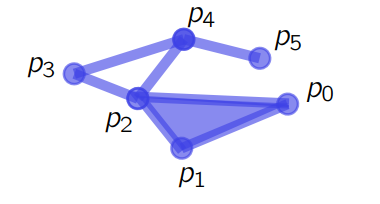
\includegraphics{image/3.png}
    \caption{}
    \label{fig:333}
\end{figure}
注意复形不一定是连通的,对于图(\ref{fig:222}),我们可以考虑下列由单形构成的集合$$K=\left\{(abc),(ab),(ac),(bc),(de),(a),(b),(c),(d),(e)\right\}$$这显然是一个复形。
\begin{figure}[htbp]
    \centering
    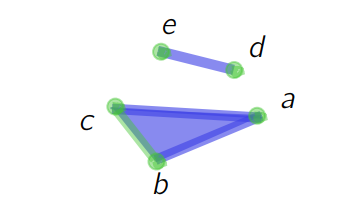
\includegraphics{image/2.png}
    \caption{}
    \label{fig:222}
\end{figure}

有了复形$K$以后,如果我们忽略掉赋予给它复形结构而只将其看作是一个点集,我们就得到了多面体的概念
\begin{definition}
给定复形$K$,则欧氏空间中的点集$\bigcup\limits_{A\in K}A$称为由$K$确定的多面体,记作$|K|$,此时我们称集合$K$为多面体$|K|$的一个三角剖分(triangulation),也称为单纯剖分,简称剖分
\end{definition}
从剖分的角度看,复形实际上赋予了一个多面体组合结构。一个多面体可以有不同构的三角剖分。
类似单形的面,我们可以定义子复形的概念
\begin{definition}
由复形$K$中的一部分单形构成的集合$L$,如果也是一个复形,则称$L$为$K$的子复形。显然$K$中所有维数小于$l$的全体单形构成$K$的一个子复形,称为$K$的$l$维骨架,记作$K^{l}$。
\end{definition}

我们至今为止讨论的构造几何图形的砖块都是平直的,然而我们只关心拓扑不变量,因此在同胚的意义下将复形的概念推广到弯曲的图形是必要的,这就是
\begin{definition}
空间$K$叫做是可剖分的,如果存在复形$K$和同胚映射$f$
\begin{equation*}
    f:|K|\longrightarrow X
\end{equation*}
这里我们称同胚映射$f$和复形$K$的二元组$(f,K)$为空间$X$的曲单纯剖分,为方便,常常不明确指出$f$
\end{definition}
当然,一个可剖分空间可以有多种曲单纯剖分,我们的目的就是确定出空间的不依赖于剖分的拓扑不变量。
为方便,我们给出下列定义
\begin{definition}
设$(f,K)$为可剖分空间$K$的一个曲单纯剖分,那么对$K$中的每一个单形$A^{k}$,我们可以得到$X$中的一个子集$f(A^{k})$,我们称这种子集为空间$X$的一个曲单形
\end{definition}
可剖分空间$X$是所有曲单形的并,至于这些曲单形是哪个单形在什么映射下的像往往不是关键的,因此我们有时也会仅仅指出可剖分空间的一组曲单形,而不指明$(f,K)$。
\begin{proposition}
可剖分空间是紧致的、可度量化的空间
\end{proposition}
\begin{proof}
只要对多面体$|K|$证明即可,首先证明多面体是紧致的。由于单形是有界闭集,而多面体是单形的有限并,从而也是有界闭的,在欧氏空间中这等价于紧致。
同样由于$|K|$是欧氏空间的子空间,从而它是可度量化的。
\end{proof}
\begin{remark}
    这一定理的逆是不成立的,由复形的构造可知,$|K|$连通等价于道路连通,因此这样的空间是不会与拓扑学家的正弦曲线同胚的。
\end{remark}
通过这一命题我们知道,并不是所有的空间都是可剖分的,好在,有很多重要的空间是可剖分的。

最后一个概念是承载单形的概念,首先需要证明如下命题
\begin{proposition}
如果点$x\in |K|$,则$K$中含有$x$的最低维单形只有一个
\end{proposition}
\begin{proof}
若K中包含点$x$的最低维单形不止一个,不妨设为$A,B$,则我们有$x\in A\bigcap B$,从而$A\bigcap B=C$是一个单形的公共面,由于$K$是复形,于是$C$也是包含$x$的一个单形,由于$A,B$为包含$x$的最低维单形,所以$C$不是它们的真面,从而有$C=A=B$,这就得到了唯一性。
\end{proof}
\begin{definition}[承载单形]
对于复形$K$,设$x\in K$,则包含$x$的最低维单形称为$x$在$K$中的承载单形,记作$\langle x\rangle_{K}$,在不引起歧义的情况下,也记为$\langle x\rangle$
\end{definition}
\begin{proposition}
\label{chap1_208}
设$A$为单形,则$x\in A^{\circ}$当且仅当$A=\langle x\rangle$
\end{proposition}
\begin{proof}
必要性:设$x\in A^{\circ}$,则由单形内点的定义,$x$的重心坐标全为正数,因为$\langle x\rangle$是$A$的面,若其为真面,则与$x$为内点矛盾,从而为$\langle x\rangle=A$。\\
充分性:若$x$不是$A$的内点,则$x$必属于$A$的边界,从而与$A$是包含$x$的维数最小单形矛盾
\end{proof}
\begin{proposition}\label{pro261}
多面体$|K|$的点$x$属于单形$A^{k}$的充要条件是$x$的承载单形为$A^{k}$的面
\end{proposition}
\begin{proof}
由定义这是显然的
\end{proof}
如果$A,B$是复形$K$的两个开单形(在单形的定义中,限制系数$\lambda_{i}>0$,即$A=A^{\circ}$),若它们相交不空,则我们必然有$x\in A^{\circ}\bigcap B^{\circ}$,根据命题(\ref{chap1_208}),我们有$\langle x\rangle=A=B$,这是因为承载单形是唯一的。这样我们得到了下列命题
\begin{proposition}
复形的任意两个不同的开单形交于空集
\end{proposition}
事实上我们有更强的结论
\begin{proposition}\label{pro272}
$\mathbb{R}^{n}$中有限个单形所构成的集合$K$被称为一个复形,如果下面的两个条件成立:
\begin{itemize}
    \item 1. 如果单形$A^{k}\in K$,则$A^{k}$的任何一个面也在$K$中;
    \item 2'. $K$的任意两个不同的开单形交于空集。
\end{itemize}
\end{proposition}
我们刚才已经证明了复形定义中的(1),(2)可以推出这里的(1),(2'),现在进行反向的证明。注意到我们只需要由命题的条件出发去证明(2)
\begin{proof}
只要证:如果单形$A$和$B$的交集$C$非空,则$C$必为它们的公共面。\\
任取$x\in C$,由于$\langle x\rangle$同时包含在$A,B$中,从而存在$A$的面$A'$和$B$的面$B'$满足$x\in A'^{\circ}$且$x\in B'^{\circ}$,即$x\in A'^{\circ}\bigcap B'^{\circ}$,由(2'),我们知道$A'=B'\subset B$,从而$A$有顶点属于$B$,记这类顶点的全体为$\left\{a_{i_{0}},\cdots,a_{i_{l}}\right\}$,从而$x\in (a_{i_{0}}\cdots a_{i_{l}})$,由$x$的任意性,我们可以得到$C\subset (a_{i_{0}}\cdots a_{i_{l}})$。\\
对于另一个方向,由于$(a_{i_{0}}\cdots a_{i_{l}})$同时是$A$和$B$的面,我们有$(a_{i_{0}}\cdots a_{i_{l}}) \subset A\bigcap B=C$,综上,我们有$A\bigcap B=(a_{i_{0}}\cdots a_{i_{l}})$,这就证明了(2)。
\end{proof}
\section{同调群}
这一节我们通过在上一节中引入的概念来引入同调群。
正如我们在最开始就提到的,同调论关心的是几何图形的边界的不变性质,为了这样的目的,首先我们要将边界这个概念严格代数化。先来看几个例子。
对于一维单形,也就是线段,我们可以知道它的边界是它的两个端点,如图(\ref{fig:293})所示。
\begin{figure}[htbp]
\centering
\begin{tikzpicture}
\coordinate (A) at (-1,0);
\coordinate (B) at (1,0);
\coordinate (A1) at ([shift={(6,0)}] A);
\coordinate (B1) at ([shift={(6,0)}] B);
\coordinate (C) at (2.2,0);
\coordinate (D) at (3.8,0);
\coordinate (M) at ($(C)!0.5!0:(D)$);
\node[above] at (M) {$\partial_{1}$};
\filldraw[black] (A1) circle (2pt)node[below]{$a_{0}$};
\filldraw[black] (B1) circle (2pt)node[below]{$a_{1}$};
\filldraw[black] (A) circle (2pt)node[below]{$a_{0}$};
\filldraw[black] (B) circle (2pt)node[below]{$a_{1}$};
\begin{scope}
  \path [draw=black,line width=1.5pt,postaction={on each segment={mid arrow=red}}] (A)node[below]{$a_{0}$}--(B)node[below]{$a_{1}$};
  \end{scope}
\draw[->] (C)--(D);
\end{tikzpicture}
    \caption{}
    \label{fig:293}
\end{figure}
上面是我们所熟知的情况,然而,如果我们考虑两个规则相处的线段构成的折线(图(\ref{fig:332})),我们留意到中间的边界点并不出现,为了能够刻画这一性质,我们给单形赋予方向,从向量(可看作有向1-单形)类比,对于一个m-单形$(a_{0}\cdots a_{m})$,我们可以从它的顶点的排列出发,给予其一个取向,从而有下面的定义

\begin{figure}[htbp]
\centering
\begin{tikzpicture}
\coordinate (A) at (-2,1);
\coordinate (O) at (0,0);
\coordinate (B) at (2.8,0);
\coordinate (A1) at ([shift={(8.5,0)}] A);
\coordinate (B1) at ([shift={(6.5,0)}] B);
\coordinate (C) at (4.0,0);
\coordinate (D) at (5.6,0);
\coordinate (M) at ($(C)!0.5!0:(D)$);
\node[above] at (M) {$\partial_{1}$};
\filldraw[black] (A) circle (2pt)node[below]{$a_{0}$};
\filldraw[black] (O) circle (2pt)node[below]{$a_{1}$};
\filldraw[black] (B) circle (2pt)node[below]{$a_{2}$};
\filldraw[black] (A1) circle (2pt)node[below]{$a_{0}$};
\filldraw[black] (B1) circle (2pt)node[below]{$a_{2}$};
\begin{scope}
  \path [draw=black,line width=1.5pt,postaction={on each segment={mid arrow=red}}] (A)node[below]{$a_{0}$}--(O)node[below]{$a_{1}$}--(B)node[below]{$a_{2}$};
  \end{scope}
\draw[->] (C)--(D);
\end{tikzpicture}
    \caption{}
    \label{fig:332}
\end{figure}
\begin{definition}[有向单形]
对于一个m-单形$(a_{0}\cdots a_{m})$,其顶点的全部排列按照奇偶性可以分成两组,我们称属于同一组的顶点排列所表示的单形具有相同的取向,而属于不同组的顶点排列所表示的单形具有相反的取向。给定了取向的m-单形被称为有向m-单形,用$\sigma^{m}$表示;与之取向相反的有向m-单形用$-\sigma^{m}$表示。\\通常我们选取与$(a_{0}a_{1}\cdots a_{m})$相同取向的单形的取向为正,记作$+(a_{0}\cdots a_{m})$或者$+\sigma^{m}$,正号可以省略;与之取向相反的有向单形的取向为负,记作$-(a_{0}\cdots a_{m})$或者$-\sigma^{m}$特别地,对于0维单形$a_{0}$,我们也规定它有两种取向,分别记为$\pm(a_{0})$。
\end{definition}
\begin{remark}
    由定义可知,取向是具有相对意义的。
\end{remark}
\begin{remark}
    同一种取向的单形的顶点排列差一个偶置换,相反取向的单形的顶点排列相差一个奇置换,因此尽管在上述定义中出现的有向单形的顶点表示均是按下标递增方式写出的,但这并不妨碍我们理解$(a_{1}a_{0}a_{2})=-(a_{0}a_{1}a_{2})$等表达式。
\end{remark}
有时我们也会通过箭头的方式标注一个有向单形的取向,例如在图(\ref{fig:293})中,我们用从$a_{0}$指向$a_{1}$的箭头来表示我们选取$(a_{0}a_{1})$取向为正,于是$(a_{1}a_{0})$取向为负,且$(a_{0}a_{1})=-(a_{1}a_{0})$
利用有向单形,我们可以给复形一个更细致的结构
\begin{definition}
设$K$为$n$维复形,它的全部单形构成的集合记为
\begin{equation*}
    \left\{A^{k}_{i}|i=1,\cdots,\phi_{k};k=0,1,\cdots,n\right\}
\end{equation*}
我们对其中每个单形取定一个取向,记作$\sigma^{k}_{i}$。对$k\in\left\{0,1,\cdots,n\right\}$,将所有$k$维有向单形做成一个集合
\begin{equation*}
    K(k)=\left\{\sigma^{k}_{i}|i=1,\cdots,\phi_{k}\right\}
\end{equation*}
我们称这个集合为$K$的一个$k$维基本组。我们将所有基本组的并记作$S(K)=\bigcup\limits_{k}K(k)$
\end{definition}
利用这一定义我们可以定义链群的概念,很快我们会看到,链群的某个子群的商群即为同调群。
\begin{definition}
对$K(k)$中任一元素$\sigma^{k}_{i}$,我们规定它在加法下的逆元素为$-\sigma^{k}_{i}$,则由$K(k)$自由生成了一个加法Abel群,我们称它为复形$K$的$k$维整数链群,记作$C_{k}(K)$
\end{definition}
\begin{remark}
    根据定义,链群中的元素$x^{k}$是下列形式和
    \begin{equation*}
        x^{k}=\sum\limits_{i=1}^{\phi_{k}}\alpha_{i}\sigma_{i}^{k},\;\alpha_{i}\in \mathbb{Z},\;i=1,\cdots,\phi_{k}
    \end{equation*}
    这个概念类似于你可以把三把椅子和两张桌子加在一起,把它们的和当作一个新的对象,当$\alpha_{i}<0$时,我们可以将其理解成$(-\alpha_{i})(-\sigma_{i})$,即理解成相反取向的单形的和。今后我们将自由地使用$\alpha_{i}\sigma^{k}_{i}$和$(-\alpha_{i})(-\sigma_{i})$这两种表达。
\end{remark}
\begin{remark}
    如果我们取$\alpha_{m}=1,\alpha_{j}=0(j\neq m)$,由此形成的链群中的元素为$1\cdot\sigma^{k}_{m}$,如果我们将$1\cdot\sigma^{k}_{m}$与$\sigma^{k}_{m}$等同起来,则我们可以认为$k$维基本组构成了$C_{k}(K)$的一组基。因此,线性代数告诉我们我们可以有多种等效的基的选择(即不同的基生成的链群同构),为了方便,如不特殊说明,在提到链群的基时,我们总是指它的$k$维基本组构成的基。
\end{remark}
\begin{definition}
当$\alpha_{i}\neq 0$时,我们定义链$\alpha_{i}\sigma_{i}^{k}$的承载复形为复形$A^{k}_{i}$,一般地,链$x^{k}=\sum\limits_{i}\alpha_{i}\sigma_{i}^{k}$的承载复形是它的所有非0项的承载复形的并。我们定义链$x^{k}$的承载体为它的承载复形所决定的多面体。
\end{definition}
因为同调论关心的是几何图形的边界,因此我们需要讲边界这个概念代数化。因为链群是一个自由群,我们所考虑的“边缘”运算应该是某种群的同态,从而只需要在一个基本组上定义边缘同态的作用。为表示最一般的情况,我们用$\epsilon(a_{0}\cdots a_{m}),\;\epsilon=\pm1$来表示顶点为$\left\{a_{0},\cdots,a_{m}\right\}$的正向或者反向单形,从而我们有
\begin{definition}
对于$k\geq1,\;k\in\mathbb{Z}$,在链群$C_{k}$的基本组与$C_{k-1}$之间,我们定义边缘运算$\partial_{k}$为
\begin{equation*}
\begin{aligned}
    \partial_{k}:\quad K(k)&\longrightarrow C_{k-1}(K)\\
    \partial_{k}(\epsilon(a_{0}a_{1}\cdots a_{k}))=&\sum\limits_{i=0}^{k}\epsilon(-1)^{i}(a_{0}a_{1}\cdots\hat{a}_{i}\cdots a_{k})
    \end{aligned}
\end{equation*}
其中$\hat{a_{i}}$表示该顶点不出现,即
\begin{equation*}
    (a_{0}\cdots\hat{a}_{i}\cdots a_{k})=(a_{0}\cdots{a}_{i-1}a_{i+1}\cdots a_{k})
\end{equation*}
特别地,我们规定0维单形的边缘为0。\\
将这一运算线性扩充后,我们得到链群$C_{k}(K)$到$C_{k-1}(K)$的同态,仍记为$\partial_{k}$。
\end{definition}
\begin{remark}
在这一定义下,我们可能需要验证$\partial_{k}((-\alpha)(-\sigma))=\partial_{k}(\alpha\sigma)$,不过这是显然的
\end{remark}
下面来看几个例子
首先我们仍考察上文中出现的线段的例子。在图(\ref{fig:293})中,$\partial_{1}(a_{0}a_{1})=(-1)^{0}(a_{1})+(-1)^{1}(a_{0})=a_{1}-a_{0}$,此外对于更高维的单形,我们有\\
$\partial_{2}(a_{0}a_{1}a_{2})=(a_{1}a_{2})-(a_{0}a_{2})+(a_{0}a_{1})$\\
$\partial_{3}(a_{0}a_{1}a_{2}a_{3})=(a_{1}a_{2}a_{3})-(a_{0}a_{2}a_{3})+(a_{0}a_{1}a_{3})-(a_{0}a_{1}a_{2})$\\
可见这确实是我们直观上的边缘概念的代数化。

由于$\partial_{k}$是两个向量空间之间的线性变换,所以我们可以引入关联矩阵的概念
\begin{definition}
我们将边缘同态在$C_{k}(K)$的一个基本组下的作用记为
\begin{equation*}
    \partial_{k}(\sigma^{k}_{i})=\sum\limits_{j=0}^{\phi_{k}}\alpha^{k}_{ij}\sigma^{k-1}_{j},
\end{equation*}
其中$\alpha^{k}_{ij}$叫做有向单形$\sigma^{k}_{i}$和$\sigma^{k-1}_{j}$之间的关联数,矩阵$(\alpha^{k}_{ij})_{1\leq i\leq\phi_{k};1\leq j\leq\phi_{k-1}},\;k=1,2,\cdots,dimK$,被称为$K$的第$k$个关联矩阵,有时也记作$(\partial_{k})$
\end{definition}
直观来看,一个图形的边缘本身应该是没有边的,我们可以将这一直观感受具体为下列命题
\begin{proposition}
设$\partial_{k+1}$和$\partial_{k}$都是边缘同态,则$\partial_{k+1}\partial_{k}=0,\;k\geq 0$
\end{proposition}
\begin{proof}
由边缘同态的定义,只需要对$C_{k+1}(K)$的基本组中的元素进行验证,此外,因为我们定义$\partial_{0}$是零同态,所以只需要验证$k\geq 1$的情况。任取$\sigma^{k+1}_{i}=\epsilon(a_{0}\cdots a_{k}a_{k+1})$,直接计算,在下面的计算中,我们约定如果求和号下标大于上标则这一项为0,容易验证这一约定是合理的。
\begin{equation*}
\begin{aligned}
    \partial_{k}\partial_{k+1}\sigma^{k+1}_{i}&=\epsilon\sum\limits_{i=0}^{k+1}(-1)^{i}\partial_{k}((a_{0}\cdots \hat{a}_{i}\cdots a_{k+1}))\\
    &=\epsilon\sum\limits_{i=0}^{k+1}(-1)^{i}\left(\sum\limits_{j=1}^{i-1}(-1)^{j}(a_{0}\cdots\hat{a}_{j}\cdots \hat{a}_{i}\cdots a_{k+1})+\sum\limits_{j=i+1}^{k}(-1)^{j-1}(a_{0}\cdots\hat{a}_{i}\cdots \hat{a}_{j}\cdots a_{k+1})\right)\\
    &=\epsilon\sum\limits_{i=1}^{k}(-1)^{i}\left(\sum\limits_{j=0}^{i-1}(-1)^{j}(a_{0}\cdots\hat{a}_{j}\cdots \hat{a}_{i}\cdots a_{k+1})+\sum\limits_{j=i+1}^{k+1}(-1)^{j-1}(a_{0}\cdots\hat{a}_{i}\cdots \hat{a}_{j}\cdots a_{k+1})\right)+\\&\quad\epsilon\sum\limits_{j=1}^{k+1}(-1)^{0}(-1)^{j-1}(a_{1}\cdots \hat{a}_{j}\cdots a_{k+1})+\epsilon\sum\limits_{j=0}^{k}(-1)^{k+1}(-1)^{j}(a_{0}\cdots \hat{a}_{j}\cdots a_{k})\\
    &=\epsilon\sum\limits_{i=1}^{k}(-1)^{i}\left(\sum\limits_{j=1}^{i-1}(-1)^{j}(a_{0}\cdots\hat{a}_{j}\cdots \hat{a}_{i}\cdots a_{k+1})+\sum\limits_{j=i+1}^{k}(-1)^{j-1}(a_{0}\cdots\hat{a}_{i}\cdots \hat{a}_{j}\cdots a_{k+1})\right)+
    \\&\quad\textcolor{red}{\epsilon\sum\limits_{j=1}^{k}(-1)^{0}(-1)^{j-1}(a_{1}\cdots \hat{a}_{j}\cdots a_{k+1})}+\textcolor{gray}{\epsilon(-1)^{k}(a_{1}\cdots a_{k})}+
    \\&\quad\textcolor{blue}{\epsilon\sum\limits_{j=1}^{k}(-1)^{k+1}(-1)^{j}(a_{0}\cdots \hat{a}_{j}\cdots a_{k})}+\textcolor{gray}{\epsilon(-1)^{k+1}(a_{1}\cdots a_{k})}+
    \\&\quad\textcolor{red}{\epsilon\sum\limits_{i=1}^{k}(-1)^{i}(-1)^{0}(a_{1}\cdots \hat{a}_{i}\cdots a_{k+1})}+\textcolor{blue}{\epsilon\sum\limits_{i=1}^{k}(-1)^{i}(-1)^{k+1-1}(a_{0}\cdots \hat{a}_{i}\cdots a_{k})}\\
    &=\epsilon\sum\limits_{i=1}^{k}(-1)^{i}\left(\sum\limits_{j=1}^{i-1}(-1)^{j}(a_{0}\cdots\hat{a}_{j}\cdots \hat{a}_{i}\cdots a_{k+1})+\sum\limits_{j=i+1}^{k}(-1)^{j-1}(a_{0}\cdots\hat{a}_{i}\cdots \hat{a}_{j}\cdots a_{k+1})\right)
\end{aligned}
\end{equation*}
由此可见在上面的第二行中出现的$k+2$项的和式中,所有含有$\hat{a}_{0}$或者$\hat{a}_{k+1}$的项可以相互抵消,因此如果$k$为偶数,则命题成立,当$k$为奇数时,记$\tilde{k}=\frac{k+1}{2}$,最后的和式化为
\begin{equation*}
     \partial_{k}\partial_{k+1}\sigma^{k+1}_{i}=\epsilon(-1)^{\tilde{k}}\left(\sum\limits_{j=\tilde{k}}^{\tilde{k}-1}(-1)^{j}(a_{0}\cdots\hat{a}_{j}\cdots \hat{a}_{\tilde{k}}\cdots a_{k+1})+\sum\limits_{j=\tilde{k}+1}^{k}(-1)^{\tilde{k}}(a_{0}\cdots\hat{a}_{\tilde{k}}\cdots \hat{a}_{j}\cdots a_{k+1})\right)=0
\end{equation*}
综上我们就证明了命题。
\end{proof}
\begin{corollary}
对于关联矩阵$(\partial_{k})$和$(\partial_{k+1})$($k\geq0$),我们有$(\partial_{k})(\partial_{k+1})=0$
\end{corollary}
现在我们已经实现了将边缘这一直观概念代数化的任务,同时也有了描述几何图形的链的概念,因此现在我们可以重新回到刻画拓扑不变量的主线任务上去。如果一个图形是另一个图形的边,即它是$\Ima(\partial_{k+1})$中的元素,因为我们从直观期望边缘关系在同胚下是不变的,所以这类元素是显然的拓扑不变量,我们对他们没有太多兴趣;另一方面,刚才的定理告诉我们边缘的边缘是零,从而一个$k$链$\sigma^{k}_{i}$是边缘的必要条件是$\sigma^{k}_{i}\in \Ker(\partial_{k})$,尽管我们有$\Ima(\partial_{k+1})\subset \Ker(\partial_{k})$,但是我们没有理由认为$\Ima(\partial_{k+1})$和$\Ker(\partial_{k})$之间存在相等的关系,考虑$\Ker(\partial_{k})$对$\Ima(\partial_{k+1})$的商群,即得到同调群的概念。从我们之前的讨论可以知道,同调群刻画的是满足边缘的必要条件而又不是边缘的几何图形在相差一个边缘的意义下的等价类。

我们将之前的讨论总结起来,得到下面更加抽象的代数的定义。
\begin{definition}
n维复形$K$的单纯链复形(或称为有向链复形、链复形),记为$C_{*}(K)$,是指如下序列:
\begin{equation*}
    \cdots\rightarrow0\rightarrow C_{n}(K)\xrightarrow{\partial_{n}}C_{n-1}(K)\xrightarrow{\partial_{n-1}}\cdots \xrightarrow{\partial_{2}}C_{1}(K)\xrightarrow{\partial_{1}}C_{0}(K)\xrightarrow{\partial_{0}}0
\end{equation*}
 其中我们要求同态之间满足$\partial_{k}\partial_{k+1}=0(k\geq 0)$
\end{definition}
\begin{definition}
我们定义复形$K$的链群的两个子群如下,分别称之为复形$K$的$k$维闭链群和$k$维边缘链群
\begin{equation*}
    \begin{aligned}
         Z_{k}(K)&=\Ker(\partial_{k})=\left\{z^{k}|z_{k}\in C_{k}(K),\partial_{k}(z^{k})=0\right\}\\
         B_{k}(K)&=\Ima(\partial_{k+1})=\left\{b^{k}|b_{k}\in C_{k}(K),\exists x^{k+1}\in C_{k+1}(K)\;s.t.\;\partial_{k+1}(x^{k+1})=b^{k}\right\}\\
    \end{aligned}
\end{equation*}
我们称$z^{k}\in Z_{k}(K)$为$k$维闭链,$b^{k}\in B_{k}(K)$为$k$维边缘链
\end{definition}
\begin{remark}
根据我们之前的讨论,$B_{k}(K)\subset Z_{k}(K)$,且由于它们都是自由群$C_{k}(K)$的子群,从而它们都是自由群
\end{remark}
\begin{definition}
商群$H_{k}(K)=Z_{k}(K)/B_{k}(K)=\Ker(\partial_{k})/\Ima(\partial_{k+1})$称为复形$K$的$k$维同调群。\\
同调群$H_{k}(K)$中的元为$Z_{k}(K)$模$B_{k}(K)$的等价类$[z^{k}]$,在上下文没有歧义时也可以写为类$z^{k}$,称之为$K$的$k$维同调类,同一同调类中的元$z_{1}^{k},z_{2}^{k}$称为是同调的,记作$z_{1}^{k}\sim z^{k}_{2}$,特别地,我们称同调于$0$的元素为零调的。
\end{definition}
显然,$B_{k}(K)$中的元素都是零调的。

根据商群的定义,我们有如下命题成立
\begin{proposition}
设$k$维闭链$x^{k}_{i}$为同调类$[x^{k}_{i}]$的代表元素,$\alpha_{i}\in \mathbb{Z}$,则等式$\sum\limits_{i}\alpha_{i}[x_{i}^{k}]=0$成立的充分必要条件是$\sum\limits_{i}\alpha_{i}x_{i}^{k}\sim0$
\end{proposition}
利用定义,我们已经可以知道一些非常平凡的同调群的结构了
\begin{proposition}
设$K$是一个$n$维复形,我们有$H_{0}(K)=C_{0}(K)/B_{0}(K)$,$H_{n}(K)=Z_{n}(K)$,当$k>n$时,$H_{k}(K)=0$
\end{proposition}
\begin{proof}
由定义,$\Ker(\partial_{0})=C_{0}(K)$,从而第一个论断成立。由于没有$n+1$维链,$C_{n+1}(K)=0$,从而$B_{n}(K)=0$,从而第二个论断成立,类似地,第三个论断成立。
\end{proof}
\begin{proposition}
边缘同态$\partial_{k}$诱导出同构$C_{k}(K)/Z_{k}(K)\cong B_{k-1}(K)$
\end{proposition}
\begin{proof}
由于$B_{k-1}(K)=\Ima(\partial_{k})$,从而由第一同构定理立得
\end{proof}

下面我们来计算几个不那么平凡的同调群。
\begin{figure}[htbp]
    \centering
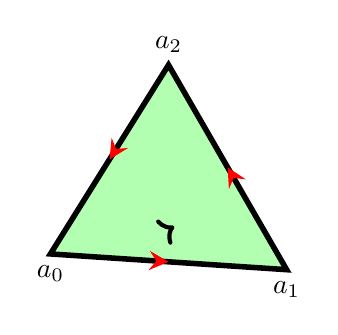
\begin{tikzpicture}
\coordinate (A) at (-1.5,-0.9);
\coordinate (B) at (1.5,-1.1);
\coordinate (C) at (0,1.5);
\coordinate (O) at (0,0);
\begin{scope}
  \path [draw=black,fill=green!30,line width=2pt,postaction={on each segment={mid arrow=red}}]
  (A)node[below]{$a_{0}$}--(B)node[below]{$a_{1}$}--(C)node[above]{$a_{2}$}--cycle;
  \end{scope}
  \begin{scope}
  \path [draw=black,->,line width=1.5pt]
  arc(75:300:0.3);
  \end{scope}
\end{tikzpicture}
    \caption{}
    \label{fig:499}
\end{figure}

\begin{figure}[htbp]
\begin{minipage}{0.3\linewidth}
\centering
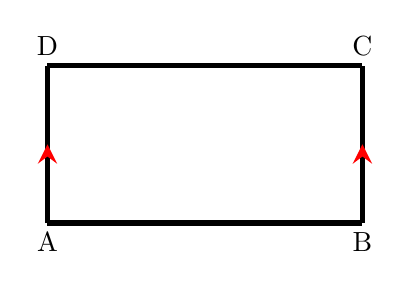
\begin{tikzpicture}
\coordinate (A) at (-2,-1);
\coordinate (B) at (2,-1);
\coordinate (C) at (2,1);
\coordinate (D) at (-2,1);
\node[below]  at (A){A};
\node[below]  at (B){B};
\node[above]  at (D){D};
\node[above]  at (C){C};
\draw [black,line width=2pt](A)--(B);
\draw [black,line width=2pt](C)--(D);
\begin{scope}
  \path [draw=black,line width=2pt,postaction={on each segment={mid arrow=red}}]
  (A)--(D);
  \end{scope}
   \path [draw=black,line width=2pt,postaction={on each segment={mid arrow=red}}]
  (B)--(C);
\end{tikzpicture}
\caption*{(a)}
\end{minipage}
\hfill
\begin{minipage}{0.3\linewidth}
\centering
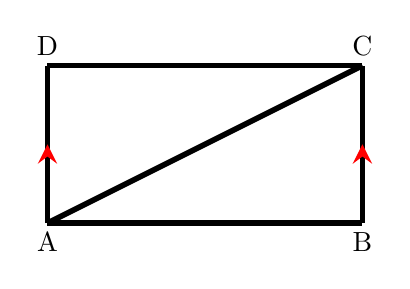
\begin{tikzpicture}
\coordinate (A) at (-2,-1);
\coordinate (B) at (2,-1);
\coordinate (C) at (2,1);
\coordinate (D) at (-2,1);
\node[below]  at (A){A};
\node[below]  at (B){B};
\node[above]  at (D){D};
\node[above]  at (C){C};
\draw [black,line width=2pt](A)--(B);
\draw [black,line width=2pt](C)--(D);
\draw [black,line width=2pt](A)--(C);
\begin{scope}
  \path [draw=black,line width=2pt,postaction={on each segment={mid arrow=red}}]
  (A)--(D);
  \end{scope}
   \path [draw=black,line width=2pt,postaction={on each segment={mid arrow=red}}]
  (B)--(C);
\end{tikzpicture}
\caption*{(b)}
\end{minipage}
\hfill
\begin{minipage}{0.3\linewidth}
\centering
\begin{tikzpicture}
\coordinate (A) at (-2,-1);
\coordinate (B) at (2,-1);
\coordinate (C) at (2,1);
\coordinate (D) at (-2,1);
\coordinate (M) at ($(A)!0.5!0:(B)$);
\coordinate (N) at ($(C)!0.5!0:(D)$);
\node[below]  at (A){A};
\node[below]  at (B){B};
\node[above]  at (D){D};
\node[above]  at (C){C};
\node[above]  at (N){N};
\node[below]  at (M){M};
\draw [black,line width=2pt](A)--(B);
\draw [black,line width=2pt](A)--(N)--(M)--(C);
\draw [black,line width=2pt](C)--(D);
\begin{scope}
  \path [draw=black,line width=2pt,postaction={on each segment={mid arrow=red}}]
  (A)--(D);
  \end{scope}
   \path [draw=black,line width=2pt,postaction={on each segment={mid arrow=red}}]
  (B)--(C);
\end{tikzpicture}
\caption*{(c)}
\end{minipage}
\caption{}
\label{fig:564}
\end{figure}
\begin{figure}
    \centering
\begin{tikzpicture}
\begin{scope}
\coordinate (A) at (-1,-1.5);
\coordinate (B) at (1,-1.5);
\coordinate (C) at (1,1.5);
\coordinate (D) at (-1,1.5);
\coordinate (E) at ($1/3*($(A)+(C)+(D)$)$);
\coordinate (F) at ($1/3*($(B)+(C)+(A)$)$);
\node[below]  at (A){$a_{1}$};
\node[below]  at (B){$a_{2}$};
\node[above]  at (C){$a_{5}$};
\node[above]  at (D){$a_{4}$};
\path [draw=black,line width=2pt,->]($(E)+(0.1,0.3)$) arc(75:300:0.25);
\path [draw=black,line width=2pt,->](F) arc(75:300:0.25);
\path [draw=black,line width=2pt,postaction={on each segment={mid arrow=red}}](-1,-1.5)--(-1,1.5)--(1,1.5);
\path [draw=black,line width=2pt,postaction={on each segment={mid arrow=red}}](-1,-1.5)--(1,-1.5)--(1,1.5);
\path [draw=black,line width=2pt,postaction={on each segment={mid arrow=red}}](-1,-1.5)--(1,1.5);
\end{scope}
\begin{scope}[shift={(2,0)}]
\coordinate (A) at (-1,-1.5);
\coordinate (B) at (1,-1.5);
\coordinate (C) at (1,1.5);
\coordinate (D) at (-1,1.5);
\coordinate (E) at ($1/3*($(A)+(C)+(D)$)$);
\coordinate (F) at ($1/3*($(B)+(C)+(A)$)$);
\node[below]  at (B){$a_{3}$};
\node[above]  at (C){$a_{6}$};
\path [draw=black,line width=2pt,->]($(E)+(0.1,0.3)$) arc(75:300:0.25);
\path [draw=black,line width=2pt,->](F) arc(75:300:0.25);
\path [draw=black,line width=2pt,postaction={on each segment={mid arrow=red}}](-1,-1.5)--(-1,1.5)--(1,1.5);
\path [draw=black,line width=2pt,postaction={on each segment={mid arrow=red}}](-1,-1.5)--(1,-1.5)--(1,1.5);
\path [draw=black,line width=2pt,postaction={on each segment={mid arrow=red}}](-1,-1.5)--(1,1.5);
\end{scope}
\begin{scope}[shift={(4,0)}]
\coordinate (A) at (-1,-1.5);
\coordinate (B) at (1,-1.5);
\coordinate (C) at (1,1.5);
\coordinate (D) at (-1,1.5);
\coordinate (E) at ($1/3*($(A)+(C)+(D)$)$);
\coordinate (F) at ($1/3*($(B)+(C)+(A)$)$);
\node[below]  at (B){$a_{1}$};
\node[above]  at (C){$a_{4}$};
\path [draw=black,line width=2pt,->]($(E)+(0.1,0.3)$) arc(75:300:0.25);
\path [draw=black,line width=2pt,->](F) arc(75:300:0.25);
\path [draw=black,line width=2pt,postaction={on each segment={mid arrow=red}}](-1,-1.5)--(-1,1.5)--(1,1.5);
\path [draw=black,line width=2pt,postaction={on each segment={mid arrow=red}}](-1,-1.5)--(1,-1.5)--(1,1.5);
\path [draw=black,line width=2pt,postaction={on each segment={mid arrow=red}}](-1,-1.5)--(1,1.5);
\end{scope}
\end{tikzpicture}
    \caption{}
    \label{fig:my_label}
\end{figure}

\begin{figure}
    \centering
\begin{tikzpicture}
\begin{scope}
\coordinate (A) at (-1,-1.5);
\coordinate (B) at (1,-1.5);
\coordinate (C) at (1,1.5);
\coordinate (D) at (-1,1.5);
\coordinate (E) at ($1/3*($(A)+(C)+(D)$)$);
\coordinate (F) at ($1/3*($(B)+(C)+(A)$)$);
\node[below]  at (A){$a_{1}$};
\node[below]  at (B){$a_{2}$};
\node[above]  at (C){$a_{5}$};
\node[above]  at (D){$a_{4}$};
\path [draw=black,line width=2pt,->]($(E)+(0.1,0.3)$) arc(75:300:0.25);
\path [draw=black,line width=2pt,->](F) arc(75:300:0.25);
\path [draw=black,line width=2pt,postaction={on each segment={mid arrow=red}}](-1,-1.5)--(-1,1.5)--(1,1.5);
\path [draw=black,line width=2pt,postaction={on each segment={mid arrow=red}}](-1,-1.5)--(1,-1.5)--(1,1.5);
\path [draw=black,line width=2pt,postaction={on each segment={mid arrow=red}}](-1,-1.5)--(1,1.5);
\end{scope}
\begin{scope}[shift={(2,0)}]
\coordinate (A) at (-1,-1.5);
\coordinate (B) at (1,-1.5);
\coordinate (C) at (1,1.5);
\coordinate (D) at (-1,1.5);
\coordinate (E) at ($1/3*($(A)+(C)+(D)$)$);
\coordinate (F) at ($1/3*($(B)+(C)+(A)$)$);
\node[below]  at (B){$a_{3}$};
\node[above]  at (C){$a_{6}$};
\path [draw=black,line width=2pt,->]($(E)+(0.1,0.3)$) arc(75:300:0.25);
\path [draw=black,line width=2pt,->](F) arc(75:300:0.25);
\path [draw=black,line width=2pt,postaction={on each segment={mid arrow=red}}](-1,-1.5)--(-1,1.5)--(1,1.5);
\path [draw=black,line width=2pt,postaction={on each segment={mid arrow=red}}](-1,-1.5)--(1,-1.5)--(1,1.5);
\path [draw=black,line width=2pt,postaction={on each segment={mid arrow=red}}](-1,-1.5)--(1,1.5);
\end{scope}
\begin{scope}[shift={(4,0)}]
\coordinate (A) at (-1,-1.5);
\coordinate (B) at (1,-1.5);
\coordinate (C) at (1,1.5);
\coordinate (D) at (-1,1.5);
\coordinate (E) at ($1/3*($(A)+(C)+(D)$)$);
\coordinate (F) at ($1/3*($(B)+(C)+(A)$)$);
\node[below]  at (B){$a_{4}$};
\node[above]  at (C){$a_{1}$};
\path [draw=black,line width=2pt,->]($(E)+(0.1,0.3)$) arc(75:300:0.25);
\path [draw=black,line width=2pt,->](F) arc(75:300:0.25);
\path [draw=black,line width=2pt,postaction={on each segment={mid arrow=red}}](-1,-1.5)--(-1,1.5)--(1,1.5);
\path [draw=black,line width=2pt,postaction={on each segment={mid arrow=red}}](-1,-1.5)--(1,-1.5);
\path [draw=black,line width=2pt,postaction={on each segment={mid arrow=red}}](1,1.5)--(1,-1.5);
\path [draw=black,line width=2pt,postaction={on each segment={mid arrow=red}}](-1,-1.5)--(1,1.5);
\end{scope}
\end{tikzpicture}
    \caption{}
    \label{fig:my_label}
\end{figure}
\section{零维同调群$H_{0}(K)$的计算}
有了上面几个例子的铺垫,我们可以来谈论稍微广泛一点的情况,根据我们目前所拥有的工具,零维同调群可以得到比较彻底的讨论。我们先来讨论一个简单的情况,倘若复形$K$的任意两个顶点$a,b$可以由多个首尾相接的一维复形连接起来,由于一维复形的两个顶点是同调的,从而我们有$a\sim b$,于是$K$的任意两个顶点均同调,$H_{0}(K)=\mathbb{Z}$。下面我们引入一系列新的概念来将这一观察重新表述。
\begin{definition}
我们称复形$K$的两个顶点$a,b$为可连接的,如果存在$K$的有限个顶点$a_{0},a_{1},\cdots,a_{k}$,其中$a_{0}=a,\;a_{k}=b$,使得$a_{i},a_{i+1}(i=0,1,\cdots,k-1)$时$K$的一个1-单形。特别地,我们规定一个顶点总是与它自己是可连接的。
\end{definition}
形象的说,如果$a,b$是可连接的,则我们可以用集合$K$中的折线将它们连接起来。

\begin{proposition}
在复形$K$中,顶点之间的可连接性是一个等价关系。在该等价关系下,属于同一个类的顶点在$K$中所张成的多个单形的集合构成$K$的一个子复形,被称为$K$的一个组合分支。
\end{proposition}
\begin{proof}
第一个论断是显然的。为证明第二个论断,我们利用复形的等价定义(\ref{pro272})。由组合分支的定义,$(1)$是成立的,因为$K$是一个复形,而组合分支中的元素仍然是$K$中的元素,从而$(2')$成立。
\end{proof}
\begin{definition}
复形$K$称为是连通的,如果它只有一个组合分支。
\end{definition}
从而我们在本节最开始讨论的其实是连通复形的情况,从而我们有如下命题
\begin{proposition}\label{pro711}
如果复形$K$连通,那么$H_{0}(K)=\mathbb{Z}$
\end{proposition}
我们可以将上述情况推广到更一般的情况
\begin{proposition}\label{pro715}
如果复形$K$有$q$个组合分支$K_{1},\cdots,K_{q}$,那么$H_{k}(K)=H_{k}(K_{1})\oplus\cdots\oplus H_{k}(K_{q})$
\end{proposition}
\begin{corollary}
若复形$K$有$q$个组合分支,则$H_{0}(K)=\bigoplus\limits_{l=1}^{q}\mathbb{Z}$
\end{corollary}
下面我们来看命题(\ref{pro715})的证明。
\begin{proof}
由于组合分支构成了$K$的一个划分,所以我们有下列关系
\begin{equation*}
\begin{aligned}
         &K=\bigcup\limits_{i=1}^{q}K_{i}\\
         &K_{i}\bigcap K_{j}=\varnothing,1\leq i\neq j \leq q
\end{aligned}
\end{equation*}
由自由生成Abel群的性质,我们有
\begin{equation*}
    C_{k}(K)=\bigoplus\limits_{l=1}^{q}C_{k}(K_{l})
\end{equation*}
而且对于$C_{k}(K_{l})$上的边缘算子$\partial_{l}$我们有
\begin{equation*}
    \partial_{l}=\partial\left.\right|_{C_{k}(K_{l})}
\end{equation*}
任取$z_{k}\in Z_{k}(K)$,从而由上式我们有$z_{k}=\sum\limits_{l=1}^{q}z_{k}^{l},\;z^{l}_{k}\in C_{k}(K_{l})$,而且由直和可知上述分解是唯一的,利用边缘算子的线性,我们有$\sum\limits_{l=1}^{q}\partial z_{k}^{l}=\partial_{l} z_{k}^{l}=0$
,从而$\partial z_{k}^{l}\in C_{k-1}(K_{l})$,利用$H_{k-1}(K)$的直和分解,我们有
\begin{equation*}
    \partial z_{k}^{l}=0
\end{equation*}
从而$Z_{k}\subset \bigoplus\limits_{l=1}^{q}Z_{k}(K_{l}) $
而反过来的方向是显然的,所以我们有
\begin{equation*}
Z_{k}(K)= \bigoplus\limits_{l=1}^{q}Z_{k}(K_{l})
\end{equation*}
类似地,我们有
\begin{equation*}
B_{k}(K)= \bigoplus\limits_{l=1}^{q}B_{k}(K_{l})
\end{equation*}
我们构造同态
\begin{equation*}
    \begin{aligned}
             \phi&:Z_{k}(K)\longrightarrow \bigoplus\limits_{l=1}^{q}H_{k}(K_{l})\\
             \phi&(z_{k})=\phi(\sum\limits_{l}z_{k}^{l})=\sum\limits_{l}[z_{k}^{l}]
    \end{aligned}
\end{equation*}
其中$z_{k}^{l}\in Z_{k}(K_{l}),\;[z^{i}_{k}]\in H_{k}(K_{l})$。显然这是一个满射,且$\Ker(\phi)=\bigoplus\limits_{l=1}^{q}B_{k}(K_{l})=B_{k}(K)$,从而由第一同构定理我们有
\begin{equation*}
    Z_{k}(K)/B_{k}(K)\cong \bigoplus\limits_{l=1}^{q}H_{k}(K_{l})
\end{equation*}
这样我们就证明了这一命题。
\end{proof}
在实际应用中,复形的连通分支的判断并不直观,下面我们将讨论复形$K$连通的充要条件。
正如我们所提到过的,我们在这里所谈论的连通的概念指的是任意两个顶点可以用一系列折线连接起来,我们事实上可以证明下列更强的命题
\begin{proposition}\label{pro767}
如果复形$K$是连通的,那么$|K|$道路连通。
\end{proposition}
\begin{proof}
对于$|K|$中任意两点$x,y$,不妨设$A$和$B$分别是包含$x$和$y$的$K$的单形,任取$A,B$的顶点分别是$a,b$,那么$x,a$和$y,b$分别构成了单形$A,B$中的一个线段,分别记作$[x,a],[b,y]$(如果存在重合的情况,则线段退化为一个点),由于$K$连通,则$a,b$可由一段折线连接起来,记作$[a,b]$,从而$[x,a],[a,b],[b,y]$构成了一条从$x$到$y$的道路。由于$x,y$的任意性,我们证明了这个命题。
\end{proof}
这个命题的逆命题也是成立的,即
\begin{proposition}\label{pro774}
如果多面体$|K|$是道路连通的,则$K$连通
\end{proposition}
为了证明这一命题,我们需要做一些直观上的解释和准备。由于连通要求的是一条特殊的道路,因此我们当然不可能直接期望道路连通性给出的道路就是我们所期望的折线,所以我们要做的是将这一条初始直线转换成我们所期望的折线。由复形的性质,如果两个顶点同属一个单形,则他们之间是可以通过1-单形连接的。我们考虑以某个顶点$a$为承载单形的顶点的集合$St_{K}(a)$,由于复形中的任意点都有承载单形,所以所有这样的集合实际构成了复形的某种覆盖,每个这样集合内的点都可以与顶点$a$建立线性连线,倘若我们能用这样的集合覆盖整条道路,注意到如果这样的集合存在公共部分$\eta$,则由承载单形的唯一性,包含$\eta$的两个集合$St_{K}(a),St_{K}(b)$必定满足$a,b$同属$\eta$的承载单形,从而可用1-单形连接,重复这样的步骤,我们就达到了我们的目的。下面来处理细节
\begin{definition}
设$K$为复形,$a$为$K$的顶点,我们定义$St_{K}(a)=\left\{x|x\in K,a\in\langle x\rangle\right\}$
\end{definition}
\begin{proposition}
$x\in St_{K}(a)$等价于$x\in|K|\backslash\bigcup\limits_{a\notin A}A$,其中$A$为$K$中单形
\end{proposition}
\begin{proof}
充分性:设$x\in St_{K}(a)$。假如$x\in|K|\backslash\bigcup\limits_{a\notin A}A$不成立,则$x\in\bigcup\limits_{a\notin A}A$,于是存在单形$\tilde{A}$满足$x\in \tilde{A}$且不包含$a$,又因为$\langle x\rangle\subset \tilde{A}$,这与$\langle x\rangle$有一个顶点为$a$矛盾\\
必要性:设$x\in|K|\backslash\bigcup\limits_{a\notin A}A$。若$a$不是$\langle x\rangle$的顶点,则$x\in\langle x\rangle\subset \bigcup\limits_{a\notin A}A$,即$x\notin|K|\backslash\bigcup\limits_{a\notin A}A$,矛盾。
\end{proof}
\begin{corollary}\label{cor_1_788}
$St_{K}(a)$是$|K|$中的开集,从而它是$a$在$|K|$中的邻域,且$\bigcup\limits_{a\in K^{0}}St_{K}(a)$构成$|K|$的一个开覆盖。
\end{corollary}
\begin{proof}
显然每个单形是多面体$|K|$中的闭集,由于$\bigcup\limits_{a\notin A}A$是有限并,从而还是闭集,从而由上一命题,$St_{K}(a)=|K|\backslash\bigcup\limits_{a\notin A}A$知道$St_{K}(a)$是$|K|$中的开集。由我们之前的讨论知道,所有$St_{K}(a)$构成一个覆盖,从而是开覆盖
\end{proof}
\begin{corollary}
对于连接$a,b$的道路$\omega:I\rightarrow|K|$,存在足够大的正整数$N$使得$\omega(\frac{1}{N})\in St_{K}(a)$
\end{corollary}
\begin{proof}
由$St_{K}(a)$为开集且$\omega$连续立得。
\end{proof}
现在我们终于可以来证明命题(\ref{pro774})
\begin{proof}
设$a,b\in K^{0}$是复形$K$的顶点,$\omega$是连接它们的道路。我们考虑所有$St_{K}(a)$构成的开覆盖,并记$St^{-1}(a)=\omega^{-1}(St_{K}(a))$,从而由连续性,$St^{-1}(a)$是$I$的一个开覆盖,由$I$是紧致的,其lebesgue数$\delta>0$,我们取$N$足够大使得$\frac{2}{N}<\delta$,从而我们有$\omega((\frac{k-1}{N},\frac{k+1}{N}))\subset St(a_{k})$,其中$a_{k}\in K^{0}$。我们考虑一个新的函数$f:I\rightarrow |K|$,定义$f(\frac{k}{N})=a_{k}$,注意到$a_{k},a_{k+1}$都是$\omega(\frac{k}{N},\frac{k+1}{N})$中的点的承载单形的顶点,从而他们之间可以用$K$中的1-单形连接,这样我们得到了一系列顶点$a_{0}=a,a_{1},\cdots,a_{N}=b$,其中相邻的两个顶点可以由折线连接,我们将$f$扩展成分段线性函数$\tilde{f}$,则得到了$a,b$之间的一个连接,从而复形$K$是可连接的。
\end{proof}
\begin{corollary}
下列三个命题等价:\\
(1)复形$K$有$q$个组合分支\\
(2)多面体$|K|$有$q$个道路连通分支\\
(3)$H_{0}(K)=\bigoplus\limits_{l=1}^{q}\mathbb{Z}$
\end{corollary}
\begin{proof}
只有(3)推(1)或(2)是不那么显然的。根据我们刚证明的结论,(1)(2)等价,我们只需要证(3)推(1)。由于连通复形的0维同调群是$\mathbb{Z}$,如果我们设$K$有$s$个连通分支,则由命题(\ref{pro715}),$H_{0}(K)=\bigoplus\limits_{l=1}^{s}\mathbb{Z}$,但是由(3)我们知道$H_{0}(K)=\bigoplus\limits_{l=1}^{q}\mathbb{Z}$,根据自由群的性质,生成元个数(rank)不同的自由群必然不同构,从而我们有$s=q$,命题得证。
\end{proof}
\section{复形$K$的一般同调群计算}
我们在之前给出的同调群的计算例子中,并没有给出可以处理更普遍的同调群的通法,这一节就来考虑这个问题。根据同调群的定义,我们只要知道$\Ker\partial_{k}$与$\Ima\partial_{k+1}$,就可以确定k维同调群。注意到边缘同态$\partial_{k}$是一个线性变换,它的作用完全由它在所有基本组上的作用决定,换言之,如果我们只要讨论$(\partial_{k})$,就可以完全讨论清楚一个复形的所有同调群。注意到$(\partial_{k})$是一个整数矩阵,根据高等代数中的结论,任意整数矩阵$M$具有形如下列的Smith标准型(所有没写出的元素都是0)
\begin{equation*}
  \left(\begin{array}{ccccc}
     d_{1}& & & & \\
     & \ddots& & &  \\
      & &d_{k} & &  \\
       & & & &  \\
     \end{array} \right) 
\end{equation*}
其中$k=\text{rank}M$,$d_{i}$为正整数,且有$d_{i}|d_{i+1},i=1,\cdots,k-1$。我们称$d_{1},\cdots,d_{k}$为$M$的不变因子,它们完全由矩阵$M$自身决定。
\begin{proof}
我们定义的初等变换由以下几个操作组成。
\begin{itemize}
    \item 第$i$行加到第$j$行上$i\neq j$\\
    \item 改变第$i$行的符号\\
    \item 第$i$列加到第$j$列上$i\neq j$\\
     \item 改变第$i$列的符号\\
\end{itemize}
得到对角形式的证明以后补。不变因子由矩阵自身决定其实是Smith标准型的唯一性。为证明这一点,我们定义矩阵$M$所有$s$阶子式($s\leq dimM=k $)的行列式的最大公因式为$M$的$s$阶行列式因子,记作$D_{s}$。由于$\text{rankM=k}$,从而$M$必然有非零的$s$阶子式,所以$D_{s}$非零。对于化成对角型的整数矩阵而言,由于$d_{i}|d_{i+1}$,我们有$D_{k}=d_{1}\cdots d_{k}$,于是不变因子$d_{s}\frac{D_{s}}{D_{s-1}},s=1,\cdots,k$,其中我们定义$D_{0}=1$。于是,只要我们证明矩阵的秩和行列式因子在初等变换下不改变即可得到Smith标准型的唯一性。\\
秩不变是显然的。对于改变某一行的符号,显然所有$k$阶子式构成的集合在相差一个符号的意义下是不变的,记变换后的行列式因子是$\widetilde{D}_{s}$,则$D_{s}|\widetilde{D}_{s}$。对于一行加到另一行上,我们可以将含有这一和式的行展开,得到两个式子之和,其中每个都是原来矩阵的$k$阶子式,从而仍然有$D_{s}|\widetilde{D}_{s}$。对于列同样讨论,这样我们就得到了在初等变换下有$D_{s}|\widetilde{D}_{s}$。由于初等变换的可逆性,我们有$\widetilde{D}_{s}|\widetilde{\widetilde{D}}_{s}=D_{s}$。综上我们有$D_{s}=\widetilde{D}_{s}$,这样就证明了Smith标准型的唯一性。
\end{proof}
\begin{proposition}
适当选取$C_{k}(K)$和$C_{k-1}(K)$的基,边缘同态$\partial_{k}:C_{k}(K)\rightarrow C_{k-1}(K)$所对应的矩阵具有下列形式
\begin{equation*}
   \left(\begin{array}{ccccc}
     \tau^{k}_{1}& & & & \\
     & \ddots& & &  \\
      & &\tau^{k}_{m_{k}} & &  \\
       & & & &  \\
     \end{array} \right) 
\end{equation*}
其中$m_{k}$是$(\partial_{k})$的秩,$\tau^{k}_{1},\cdots,\tau^{k}_{m_{k}}$是不变因子,只由$\partial_{k}$决定,与基的选取无关
\end{proposition}
因此,如果我们把$(\partial_{k})$化成它的Smith标准型,则可以直观看出它的零空间和像空间,这相当于选定了另一组基。然而,通过$(\partial_{k})$我们可以确定的是$\Ker(\partial_{k})$和$\Ima(\partial_{k})$,不过为了计算同调群$H_{k}$我们需要的是$\Ker(\partial_{k})$和$\Ima(\partial_{k+1})$。通过$C_{k+1},C_{k}$的基的选取,我们可以确定$\Ima(\partial_{k+1})$,通过$C_{k},C_{k-1}$的基的选取,我们可以确定$\Ker(\partial_{k+1})$,一个自然的问题是,这两种情况下,$C_{k}(K)$中选取的基之间存在什么关系,一个更加大胆的想法是,这两种情况下得到的基是不是相同,即我们可以在一组$C_{k}(K)$基的选取下,同时对角化$(\partial_{k}),(\partial_{k+1})$。事实上这是完全可以做到的,我们现在就来做这件事情。\\
显然,对于一般情况我们是不可能期望这个同时对角化是可能的,但是注意到边缘同态满足$\partial_{k+1}\partial_{k}=0$,这可能会给我们带来希望。首先我们考虑将$(\partial_{k+1})$Smith对角化的一组$C_{k+1}(K)$和$C_{k}(K)$的基为$\left\{{c_{1}^{k+1},\cdots,c_{m_{k+1}}^{k+1},z_{1}^{k+1},\cdots,z_{\phi_{k}-m_{k+1}}}\right\}$和$\left\{{c_{1}^{k},\cdots,c_{m_{k+1}}^{k},z_{1}^{k},\cdots,z_{\phi_{k}-m_{k+1}}}\right\}$,我们记$\partial_{k+1}$在这组基下的矩阵为$M_{k+1}$,它是一个$\phi_{k}\times \phi_{k+1}$矩阵,满足
$M_{k+1}c_{l}^{k+1}=\tau^{k+1}_{l}c_{l}^{k},\;M_{k+1}z_{l}^{k+1}=0$,即$M_{k+1}$有形式
\begin{equation*}
	M_{k+1}=\begin{array}{c@{\hspace{-5pt}}l}	
	\left(\begin{array}{ccc|ccc}	
	\tau^{k+1}_{1}& & & & &\\	
	&\ddots & & & \\	
	& &\tau^{k+1}_{m_{k+1}}& \multicolumn{3}{c}{\raisebox{2ex}[0pt]{\Huge0}}\\\hline	
	& & & & & \\	
	& & & & & \\	
	\multicolumn{3}{c|}{\raisebox{2ex}[0pt]{\Huge0}}
	& 	\multicolumn{3}{c}{\raisebox{2ex}[0pt]{\Huge0}}	
	\end{array}\right)
	\end{array}=\left(\begin{array}{cc}
	    A^{k+1} & O \\
	    O & O 
	\end{array}\right)
	\end{equation*}
仍然取$C_{k}(K)$的基为$\left\{{c_{1}^{k},\cdots,c_{m_{k+1}}^{k},z_{1}^{k},\cdots,z_{\phi_{k}-m_{k+1}}}\right\}$,我们取$C_{k-1}$的一组基为$\tilde{c}_{1}^{k-1},\cdots,\tilde{c}_{\phi_{k-1}}^{k-1}$,并记在这组基下$\partial_{k}$的矩阵为$M_{k-1}$,我们将它写成$m_{k+1}\times(\phi_{k}-m_{k+1})$的列分块矩阵
\begin{equation*}
    \left(\begin{array}{c}
         \tilde{A}  \\
          \tilde{B}
    \end{array}\right)
\end{equation*}
,利用$M_{k+1}M_{k}=0$可知$\tilde{A}=0$,我们对$\tilde{B}$进行初等变换将其化成Smith标准型,注意此时我们只需要调整$C_{k}(K)$中的基的一个子集$\left\{{z_{1}^{k},\cdots,z_{\phi_{k}-m_{k+1}}}\right\}$,由于$M_{k+1}$中与$z^{k}$相关的列都是0,所以在将$\tilde{B}$对角化的过程中,可以保持$M_{k+1}$的形式不变,注意此时$\left\{{z_{1}^{k},\cdots,z_{\phi_{k}-m_{k+1}}}\right\}$是会发生改变的,我们记此时$C_{k}(K)$的新的基为$\left\{{c_{1}^{k},\cdots,c_{m_{k+1}}^{k},\overline{z}_{1}^{k},\cdots,\overline{z}_{\phi_{k}-m_{k+1}}}\right\}$。\\
我们将$\tilde{c}_{1}^{k-1},\cdots,\tilde{c}_{\phi_{k-1}}^{k-1}$中,属于$M_{k+1}$的像集的记作$c_{1}^{k-1},\cdots,c_{m_{k}}^{k-1}$,其余的记作$z_{1}^{k-1},\cdots,z_{\phi_{k-1}-m_{k}}^{k-1}$,则$M_{k}$有形式
\begin{equation*}
	M_{k}=\begin{array}{c@{\hspace{-5pt}}l}	
	\left(\begin{array}{ccc|ccc}
		& & & & & \\	
	& & & & & \\	
	\multicolumn{3}{c|}{\raisebox{2ex}[0pt]{\Huge0}}
	& 	\multicolumn{3}{c}{\raisebox{2ex}[0pt]{\Huge0}}	\\\hline
	\tau^{k}_{1}& & & & &\\	
	&\ddots & & & \\	
	& &\tau^{k}_{m_{k}}& \multicolumn{3}{c}{\raisebox{2ex}[0pt]{\Huge0}}
	\end{array}\right)
	\end{array}=\left(\begin{array}{cc}
	    O & O \\
	    A^{k} & O 
	\end{array}\right)
	\end{equation*}
这样我们就实现了我们一开始的目标。由我们的推导过程,我们发现可以将$C_{k}(K)$中的一组基按下列方式分成五类:首先是$\Ima\partial_{k+1}$的像的基,$A_{k}$该基所对应的不变因子为1;$B_{k}$该基所对应的不变因子不为1,剩下三类不在$\Ima\partial_{k+1}$中,分别是$U_{k}\in\Ker\partial_{k}$;$V_{k}$,该基所对应的不变因子为1;$W_{k}$,该基所对应的不变因子不为1。换言之,我们有$A_{k}=\partial_{k+1}V_{k+1},\;B_{k}=\partial_{k+1}W_{k+1}$,是我们不怎么关心的真正的边缘。$U_{k}$是我们所关心的同调群中的生成元,$V_{k},W_{k}$不是闭链中的元素。\\
\begin{proposition}
设$K$为$n$维复形,则$A_{n},B_{n}$为空集。对于任意复形,都有$V_{0},W_{0},B_{0},W_{1}$为空集。
\end{proposition}
\begin{proof}
由于$\partial_{n+1}$为0映射,所以它的像中不包含任何基向量,从而$A_{n},\;B_{n}$为空集。同理,由于$\partial_{0}$为0,从而它的任何元素的像都是0,所以$V_{0},W_{0}$是空集。由边缘算子的性质,在基本组作为基的情况下,$(\partial_{1})^{\top}$每一行都只由一个1和一个$-1$组成,而且不存在完全相同的两行。对于任意一个非零$k$子式,不妨设其中每一行都包含$1,-1$,因为只含有一个数字的行我们可以按这一行展开,得到一个$k-1$子式,然后可以重复讨论,如果有一行只有一个数字,可以继续展开,直到所有的行都有两个数字或我们可以直接得到整个行列式的值为$\pm1$。我们从第一列开始,不妨设第一列所有的非零数字都是1,然后利用初等变换,可以利用其中某一行将其他第一列的数字消掉。注意到这样得到的新的行仍然是由一个1和一个$-1$组成。利用归纳法,我们可以得到这样的矩阵的每一个行列式因子都是$\pm1$,从而所有的不变因子都是1。
\end{proof}
\begin{definition}
我们定义$(\partial_{k+1})$的秩为$\alpha_{k}$
\end{definition}
由定义可知,$(\partial_{k+1})$的秩即为$A_{k},B_{k}$中的元素数目,记为$\alpha_{k}=|A_{k}|+|B_{k}|$,因此$\alpha_{n}=0,\alpha_{0}=|A_{0}|$,特别地,我们约定$\alpha_{-1}=0$。另外由$A_{k}=\partial_{k+1}V_{k+1}$,$B_{k}=\partial_{k+1}W_{k+1}$可知$|A_{k}|=|V_{k+1}|,\;|B_{k}|=|W_{k+1}|$。
\begin{definition}
对于$n$维复形,$k=0,1,\cdots,n$,我们可以定义 $\beta_{k}=\phi_{k}-\alpha_{k}-\alpha_{k-1}$称为复形$K$的第$k$个Betti数,大于1的不变因子$\tau^{k}_{1},\cdots,\tau^{k}_{|B_{k}|}$称为复形$K$的$k$维挠系数。
\end{definition}
\begin{proposition}\label{pro902}
对于$n$维复形$K$,$H_{k}=\left(\bigoplus\limits_{l=1}^{\beta_{k}}\mathbb{Z}\right)\bigoplus\left(\bigoplus\limits_{l=1}^{|B_{k}|}\mathbb{Z}/\tau_{l}^{k}\right)$,其中$\beta_{k}$是我们刚刚定义的Betti数,$\tau_{l}^{k}$是$k$维挠系数。
\end{proposition}

\begin{proof}
由上面的讨论可以知道,$Z_{k}(K)$的一组生成元是$A_{k},B_{k},U_{k}$,而$B_{k}(K)$的一组生成元是$A_{k},\tau^{k}_{l}b_{l}$,其中$b_{l}\in B_{k}$。这样$H_{k}=\left(\bigoplus\limits_{l=1}^{|U_{k}|}\mathbb{Z}\right)\bigoplus\left(\bigoplus\limits_{l=1}^{|B_{k}|}\mathbb{Z}/\tau_{l}^{k}\right)$,但是由于$|U_{k}|=\phi_{k}-|A_{k}|-|B_{k}|-|V_{k}|-|W_{k}|=\phi_{k}-|A_{k}|-|B_{k}|-|A_{k-1}|-|B_{k-1}|=\phi_{k}-\alpha_{k}-\alpha_{k-1}=\beta_{k}$,当$k=0$时,由于$B_{0},V_{0},W_{0}$都是空集,所以$|U_{0}|=\phi_{0}-A_{0}=\phi-\alpha_{0}-\alpha_{-1}$,与我们约定$A_{-1}=0$是一致的。综上,我们就得到了命题。
\end{proof}
\begin{remark}
Betti数$\beta_{k}=\phi_{k}-\alpha_{k}-\alpha_{k-1}$,其中$\alpha_{k}$是$(\partial_{k})$的秩,这说明Betti数$\beta_{k}$和两个边缘算子$\partial_{k},\partial_{k-1}$都有关,而挠系数仅仅是矩阵$(\partial_{k+1})$的不变因子,所以挠系数由$\partial_{k+1}$完全决定,而与$\partial_{k}$无关。
\end{remark}
\begin{definition}
$n$维复形$K$的Euler示性数定义为$\chi(K)=\sum\limits_{l=0}^{n}(-1)^{l}\phi_{l}$,其中$\phi_{l}$是$K$的$k$维单形数。
\end{definition}
\begin{proposition}
$n$维复形$K$的Euler示性数和Betti数之间有关系$\chi(K)=\chi(K)=\sum\limits_{l=0}^{n}(-1)^{l}\beta_{l}$
\end{proposition}
\begin{proof}
利用$\beta_{l}=\phi_{l}-\alpha_{l}-\alpha_{l-1}$直接计算,
\begin{equation*}
    \begin{aligned}
      \sum\limits_{l=0}^{n}(-1)^{l}\beta_{l}&=\sum\limits_{l=0}^{n}(-1)^{l}(\phi_{l}-\alpha_{l}-\alpha_{l-1})\\
      &=\sum\limits_{l=0}^{n}(-1)^{l}\phi_{l}-\alpha_{-1}+(-1)^{n}\alpha_{n}\\
      &=\sum\limits_{l=0}^{n}(-1)^{l}\phi_{l}
    \end{aligned}
\end{equation*}
\end{proof}
\begin{remark}
将来我们会证明,同调群是拓扑不变的,从而Betti数是拓扑不变的,即Euler示性数是拓扑不变量。对于一个多面体$|K|$,我们可以有不同的划分,从而单形的数目$\phi_{k}$是变化的,但是Euler示性数的拓扑不变性告诉我们,他们的简单加减的组合是不变的。
\end{remark}
我们下面利用这种方法来计算一下球面的同调群。我们选取球面的四面体三角剖分,如下图所示
\begin{figure}[htpb]
    \centering
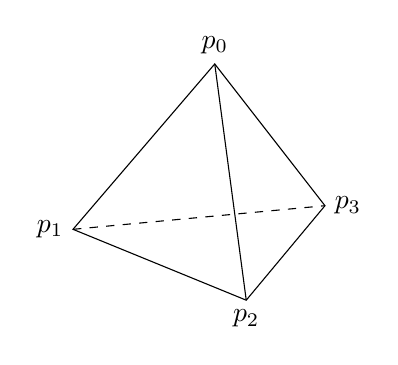
\begin{tikzpicture}
\coordinate (A0) at (-0.2,2);
\coordinate (A1) at (-2,-0.1);
\coordinate (A2) at (0.2,-1);
\coordinate (A3) at (1.2,0.2);
\node[above] at (A0){$p_{0}$};
\node[left] at (A1){$p_{1}$};
\node[below] at (A2){$p_{2}$};
\node[right] at (A3){$p_{3}$};
\draw (A0)--(A1)--(A2)--(A3)--cycle;
\draw (A0)--(A2);
\draw[dashed] (A1)--(A3);
  \end{tikzpicture}
    \caption{}
    \label{fig:my_label}
\end{figure}
我们可以写出它的各维基本组为
\begin{equation*}
    \begin{aligned}
    K(0)&=\left\{p_{0},p_{1},p_{2},p_{3}\right\}\\
     K(1)&=\left\{(p_{0}p_{1}),(p_{0}p_{2}),(p_{0}p_{3}),(p_{1}p_{2}),(p_{1}p_{3}),(p_{2}p_{3})\right\}\\
     K(3)&=\left\{(p_{1}p_{2}p_{3}),(p_{0}p_{2}p_{3}),(p_{0}p_{1}p_{3}),(p_{0}p_{1}p_{2})\right\}\\
    \end{aligned}
\end{equation*}
于是我们可以写出基本组下的边缘变换的矩阵
\begin{equation*}
    \begin{aligned}
    M_{0}&=\left(\begin{array}{cccc}
     0 & 0  &0 &0 \\
    \end{array}\right)\\
    M_{1}&=\left(\begin{array}{cccccc}
        -1 &-1&-1&0&0&0  \\
        1 &0&0&-1&-1&0\\
        0 &1&0&1&0&-1\\
        0 &0&1&0&1&1\\
    \end{array}\right)\\
    M_{2}&=\left(\begin{array}{cccc}
        0 & 0&1&1 \\
        0 & 1&0&-1 \\
        0 & -1&-1&0 \\
        1 & 0&0&1 \\
        -1 & 0&1&0 \\
        1 & 1&0&0 \\
    \end{array}\right)
    \end{aligned}
\end{equation*}
利用mma我们可以得到它们的Smith标准型
\begin{equation*}
    \begin{aligned}
    D_{0}&=\left(\begin{array}{cccc}
     0 & 0  &0 &0 \\
    \end{array}\right)\\
    D_{1}&=\left(\begin{array}{cccccc}
        1 &0&0&0&0&0  \\
        0 &1&0&0&0&0\\
        0 &0&1&0&0&0\\
        0 &0&0&0&0&0\\
    \end{array}\right)\\
    D_{2}&=\left(\begin{array}{cccc}
        1 & 0&0&0 \\
        0 & 1&0&0 \\
        0 & 0&1&0 \\
        0 & 0&0&0 \\
        0 & 0&0&0 \\
        0 & 0&0&0 \\
    \end{array}\right)
    \end{aligned}
\end{equation*}
在这个例子中,我们有$\phi_{0}=4,\phi_{1}=6,\phi_{2}=4$,$\;\alpha_{0}=\text{rank}(\partial_{1})=3,\alpha_{1}=\text{rank}(\partial_{2})=3,\alpha_{2}=0$,从而$\beta_{0}=1,\beta_{1}=0,\beta_{2}=1$,于是根据命题(\ref{pro902}),我们知道球面非平凡的同调群为$H_{0}(S^{2})=\mathbb{Z},\;H_{2}(S^{2})=\mathbb{Z}$
\section{上同调群}
我们在前面较为详尽的讨论了一些简单几何体的同调群,在那里,我们的基本方法是利用边缘同态,考察更高一维的复形在低一维的边界是怎样的,我们同样十分好奇,低一维的边界是以怎样的方式参与了高维几何体的构成,这就是这一节要讨论的上同调的概念。我们在讨论同调群是定义了关联矩阵$(\partial_{k})$,在选定一组基后,对于$C_{k}$中的链$\beta_{k}$,可以将其表示成列向量形式,且$(\partial_{k})\beta_{k}$给出了它的边缘。在$C_{k-1}$中选定一组基后,它的链都可以表成列矢量$\gamma_{k-1}$,我们注意到$(\partial_{k})^{\top}\gamma_{k-1}$是$C_{k}$中的链,而且,我们设单位向量$e_{i}$对应的$C_{k-1}$中的基为$\sigma^{k-1}$,则$(\partial_{k})^{\top}e_{i}$中的非零坐标对应了所有的边界含有$\sigma^{k-1}$的$C_{k}$中的基。\\
根据上面的讨论,我们定义
\begin{definition}[上边缘同态]
对于复形$K$的相邻的链群,我们可以定义上边缘同态为$(\delta^{k-1})=(\partial_{k})^{\top}$\\
\begin{equation*}
\begin{aligned}
    &\delta^{k-1}:C_{k-1}(K)\rightarrow C_{k}(K)\\
    &\delta^{k-1}(\sigma^{k-1}_{j})=\sum\limits_{i=1}^{\phi_{k}}\alpha_{ij}^{k}\sigma^{k}_{i}
\end{aligned}
\end{equation*}
其中$\alpha_{ij}^{k}$是我们之前定义的关联数。
\end{definition}
按我们的定义,$(\delta^{k})$右乘作用于行矢量上。
\begin{proposition}
对于上边缘同态我们有$\delta^{k}\delta^{k-1}=0$,或者对于矩阵$(\delta^{k})$而言,我们有$(\delta^{k-1})(\delta^{k})=0$
\end{proposition}
\begin{proof}
利用定义,我们有$(\delta^{k-1})=(\partial_{k})^{\top}$,从而我们有$(\delta^{k-1})(\delta^{k})=(\partial_{k})^{\top}(\partial^{k+1})^{\top}=((\partial_{k+1})(\partial_{k}))^{\top}=0$,从而我们有$\delta^{k}\delta^{k-1}=0$
\end{proof}
\begin{corollary}
$\Ima\delta^{k-1}\subset \Ker\delta^{k}$
\end{corollary}
\begin{definition}
我们定义复形$K$的$k$维上闭链群$Z^{k}(K)$和上边缘链群$B^{k}(K)$分别为$\Ker\delta^{k}$和$\Ima\delta^{k-1}$,它们的商群$H^{k}(K)=Z^{k}(K)/B^{k}(K)=\Ker\delta^{k}/\Ima\delta^{k-1}$,成为复形$K$的$k$维上同调群。
\end{definition}
由于上同调群也是由边界关系导出的,和同调群一样,我们也期望它们是拓扑不变的,事实上也的确如此,在第二章我们会证明这一点。现在我们来从另一个角度来理解上同调群。同态$\partial_{k}$和$\delta_{k-1}$的表示矩阵互为转置,这让我们想到了线性空间的对偶空间相关的命题,事实上,对于群而言,我们确实存在类似的命题,这是因为向量空间和Abel群都具有模的结构。
\begin{definition}
我们定义所有形如$f:G\rightarrow \mathbb{Z}$的同态构成的集合为$\text{Hom}(G,\mathbb{Z})$,其中$G$为Abel群。这个集合在普通的映射加法下构成一个Abel群,称之为从群$G$到$\mathbb{Z}$的同态群,记为$\text{Hom}(G,\mathbb{Z})$
\end{definition}
\begin{proposition}\label{pro1035}
设$F,G$为群,$\phi:F\rightarrow G$为群同态,则$\phi$诱导了从$\text{Hom}(G,\mathbb{Z})$到$\text{Hom}(F,\mathbb{Z})$的同态$\phi^{*}$:
\begin{equation*}
    \begin{aligned}
        \phi^{*}:\text{Hom}(G,\mathbb{Z})&\rightarrow\text{Hom}(F,\mathbb{Z})\\
        \phi^{*}(g)&=g\circ \phi
    \end{aligned}
\end{equation*}
我们称$\phi^{*}$为$\phi$诱导的对偶同态,有时也将它记作$Hom(\phi)$。
\end{proposition}
\begin{proof}
先验证$\phi^{*}(g)$为$F$到$\mathbb{Z}$的同态,随后验证$\phi^{*}$为从$\text{Hom}(G,\mathbb{Z})$到$\text{Hom}(F,\mathbb{Z})$的同态。即对任意$a,b\in F$,我们有$\phi^{*}(g)(a+b)=\phi^{*}(g)(a)+\phi^{*}(g)(b)$;以及对任意$g,g'\in\text{Hom}(G,\mathbb{Z})$,任意$a\in F$,有$\phi^{*}(g+g')(a)=(\phi^{*}(g)+\phi^{*}(g'))(a)$,细节略
\end{proof}
\begin{corollary}\label{pro1049}
对偶同态满足$Hom(g\circ f)=Hom(f)\circ Hom(g),Hom(1)=1$
\end{corollary}
\begin{proof}
对于任意$\phi\in Hom(G,\mathbb{Z})$,我们有$Hom(g\circ f)\phi=\phi\circ g\circ f=(Hom(f)\circ Hom(g))\phi$,$Hom(1)(\phi)=\phi\circ 1=\phi$
\end{proof}
对于自由群$F$而言,我们可以仿照线性空间,定义它的对偶基,从而可以证明如此得到的同态群$\text{Hom}(F,\mathbb{Z})\cong F$。链群$C_{k}(K)$是以基本组$\left\{\sigma^{k}_{i}\right\}$为基的自由群,我们记与其同构的同态群为$C^{k}(K)$,其中的基$\left\{\tau^{k}_{i}\right\}$,满足$\tau^{k}_{i}(\sigma^{k}_{j})=\delta^{ij}$。
\begin{definition}
对于复形$K$而言,我们称$C^{k}(K)$为$K$的$k$维上链群,它的元称为$k$维上链.如果记上链群中的一组基为$\left\{\tau^{k}_{i}\right\}$,则任意上链具有形式$\sum\limits_{i=1}^{\phi_{k}}\alpha_{i}\tau^{k}_{i}$
\end{definition}
根据命题(\ref{pro1035}),边缘同态诱导了同态群之间的同态$\partial_{k}^{*}$:
\begin{equation*}
\begin{aligned}
    \partial_{k}^{*}:C^{k-1}(K)&\rightarrow C^{k}(K)\\
    \partial_{k}^{*}(\tau^{k-1}_{i})&=\tau^{k-1}_{i}\circ \partial_{k}
    \end{aligned}
\end{equation*}
事实上,考虑$\partial_{k}^{*}(\tau^{k-1}_{i})$在$C_{k}(K)$上的作用,我们有
\begin{equation*}
    \begin{aligned}
    \partial_{k}^{*}(\tau^{k-1}_{i})(\sigma^{k}_{j})&=\tau^{k-1}_{i}(\partial_{k}\sigma^{k}_{j})\\
    &=\tau^{k-1}_{i}(\sum\limits_{l=1}^{\phi_{k-1}}\alpha^{k}_{jl}\sigma_{l}^{k-1})\\
    &=\alpha^{k}_{ji}\\
    &=\sum\limits_{\beta=1}^{\phi_{k}}(\alpha^{k}_{\beta i}\tau^{k}_{\beta})\sigma^{k}_{j}
    \end{aligned}
\end{equation*}
将上式进行线性扩充,我们就得到了想要的同态。由于$\left\{\sigma^{k}_{j}\right\}$是一组基,这表明
\begin{equation*}
    \partial_{k}^{*}(\tau^{k-1}_{i})=\sum\limits_{\beta=1}^{\phi_{k}}(\alpha^{k}_{\beta i}\tau^{k}_{\beta})
\end{equation*}
注意到这一变换行为与我们之前定义的$\delta^{k-1}$相同,
由于$C^{k}(K)\cong C_{k}(K)$,所以我们可以将$\sigma^{k}_{i}$和$\delta^{k}_{i}$等同起来,这样我们就可以在相差一个同构的意义下认为$\delta^{k-1}=\partial_{k}^{*}$,这样,我们可以说上边缘同态就是边缘同态的对偶,以后对于上同调,我们都采用这样对偶的说法。\\
有了对偶的概念,我们可以引入上链群和链群之间的配对
\begin{definition}
我们称下列映射$\kappa$为Kronecker指数,
\begin{equation*}
    \begin{aligned}
    &\kappa:C^{k}(K)\times C_{l}(K)\rightarrow \mathbb{Z}\\
    &\kappa(\phi,c)=\left\{\begin{array}{cc}
         0,\quad k\neq l  \\
         \phi(c),\quad k=l 
    \end{array}\right.
    \end{aligned}
\end{equation*}
有时也将$\kappa(\phi,c)$记作$\langle\phi,c \rangle$
\end{definition}
根据上链群的定义我们马上有
\begin{proposition}
(1)Kronecker指数是双线性的\\
(2)$\langle\partial^{*}_{k+1}\phi_{k},c_{k+1}\rangle=\langle\phi_{k},\partial_{k+1}c_{k+1}\rangle$
\end{proposition}
\begin{corollary}
(1)$\langle\partial_{k+1}^{*}\phi_{k},z_{k+1}\rangle$=0,对任意$\phi_{k}\in C^{k}(K),\;z_{k+1}\in Z_{k+1}(K)$成立\\
(2)$\langle\phi_{k},\partial_{k+1}c_{k+1}\rangle$=0,对任意$\phi_{k}\in Z^{k}(K),\;c_{k+1}\in C_{k+1}(K)$成立
\end{corollary}
\begin{corollary}\label{coro1098}
(1)上链$\phi\in Z^{k}(K)$的充要条件是$\langle\phi,\partial c \rangle=0$对于任意$c\in C_{k+1}(K)$成立,即$\phi$是$k$维上闭链的充要条件为$\phi$是$k$维边缘链的零化子\\
(2)上链$\psi\in B^{k}(K)$,则$\langle\psi,z\rangle=0$对于任意$z\in Z_{k}(K)$成立,即若$\psi$是$k$维上边缘链,则$\psi$是$k$维闭链的零化子
\end{corollary}
\begin{proof}
先证(1):设$\phi_{k}\in Z^{k}(K)$,则$\partial_{k+1}^{*}\phi_{k}=0$,即$0=\langle \partial_{k+1}^{*}\phi_{k},c_{k+1}\rangle=\langle \phi_{k},\partial_{k+1}c_{k+1}\rangle$,这样我们就证明了一个方向。对于另一个方向,我们设$\langle \phi_{k},\partial_{k+1}c_{k+1}\rangle=0$对任意$c$成立,则我们有$\langle \partial_{k+1}^{*}\phi_{k},c_{k+1}\rangle=0$恒成立,这表明$\partial_{k+1}^{*}\phi_{k}=0$,即$\phi_{k}\in Z^{k}(K)$\\
对于(2),我们可以设$\psi_{k}=\partial^{*}_{k-1}c_{k-1}$,则$\langle\psi_{k},z_{k}\rangle=\langle c_{k-1},\partial_{k}z_{k}\rangle=0$
\end{proof}
\begin{corollary}
$\kappa$诱导了$H^{k}(K)\times H_{l}(K)$到$\mathbb{Z}$的同态$\tilde{\kappa}$为$\tilde{\kappa}([\phi],[{Z}])=\langle\phi,z\rangle$
\end{corollary}
\begin{proof}
只要证明上述同态是良定义的。考虑到$[\phi]$中的元素属于上闭链且相差一个上边缘链,$[z]$中的元素属于闭链且相差一个边缘链,那么根据推论$(\ref{coro1098})$,我们自然有同态是良定义的。
\end{proof}
利用$\tilde{\kappa}$我们可以定义Kronecker映射导出的下列同态:
\begin{equation*}
    \begin{aligned}
    \alpha:H^{k}(K)&\rightarrow \text{Hom}(H_{k}(X),\mathbb{Z})\\
    [\phi]&\rightarrow\alpha([\phi])
    \end{aligned}
\end{equation*}
其中$\alpha([\phi])\in \text{Hom}(H_{k}(K),\mathbb{Z})$满足$\alpha([\phi])([z])=\tilde{\kappa}([\phi],[z]),\;z\in Z_{k}(K)$

与同调群一样,对于上同调群我们也有一个计算的问题,注意到我们有$(\delta^{k})=(\partial_{k+1})^{\top}$,在我们选用的ABUVW基下,可以清楚看到转置不会改变不变因子的数目,也不会改变秩,从而经过一定的基重排后我们可以以与同调群相同的讨论方式来讨论上同调群的一般求法,所以我们有
\begin{proposition}\label{pro1122}
对于$n$维复形$K$,$H^{k}=\left(\bigoplus\limits_{l=1}^{\beta_{k}}\mathbb{Z}\right)\bigoplus\left(\bigoplus\limits_{l=1}^{|B_{k-1}|}\mathbb{Z}/\tau_{l}^{k-1}\right)$,其中$\beta_{k}$是我们之前定义的Betti数,$\tau_{l}^{k-1}$是$k-1$维挠系数。
\end{proposition}
\begin{proof}
由于我们仅仅进行了矩阵的转置,因此在$(\delta^{k})$中,仍然存在不变因子为1和不变因子大于一的基,我们设$\delta^{k}D_{k}=X_{k+1},\delta^{k}E_{k}=Y_{k+1}$,其中$D_{k},E_{k}$分别是不变因子为1和不变因子大于1的基的集合。此外我们设$S_{k}$为不在$\Ima\delta_{k-1}$但在$\Ker\delta^{k}$中的基。这样,$\Ker\delta^{k}$的生成元个数是$|{S}_{k}|+|{X}_{k}|+|{Y}_{k}|$,$\Ima\delta^{k-1}$的生成元是$\tilde{X}_{k},\tau^{k-1}_{i} y_{i}$,我们注意到转置后秩是不变的,所以仍然有$|S_{k}|=\phi-\text{rank}(\delta^{k})-\text{rank}(\delta^{k-1})=\phi_{k}-\alpha_{k}-\alpha_{k-1}=\beta_{k}$,所以$H^{k}(K)$的自由部分仍然有$\beta_{k}$个,而循环群部分由$\tau^{k-1}_{i}$给出,这是由于在边缘同态中,我们是用像的编码来标识不变因子,而在上边缘同态中,我们仍然沿用这一记号,相当于我们用了定义域来编号,两者相差1。此外,当$k=0,1$时,根据同调群中的结论我们可以知道此时$\delta^{-1},\delta^{0}$的像中的基所对应的不变因子都是1,所以$H^{0}(K),H^{1}(K)$都是自由群,此时如果我们认为上标小于下标意味着这一项不存在,则命题仍然成立。
\end{proof}
\begin{corollary}
复形$K$的同调群和上同调群之间存在如下关系:\\
(1)$H_{k}(K)$和$H^{k}(K)$有相同的自由群部分;\\
(2)$H_{k}(K)$和$H^{k+1}(K)$有相同的有限子群部分
\end{corollary}
\begin{proof}
由命题(\ref{pro902})和命题(\ref{pro1122})立得
\end{proof}
由上述推论,我们可以知道同调群与上同调群之间存在着密切的关系,事实上,如果我们知道了其中的一个,就可以确定出另一个,然而,在不同的场合使用这两种语言的方便程度是不同的,所以这两种概念都是有各自的意义的。
\section{复形的运算}
之前我们介绍了由单形得到复形的操作,这一节中我们将讨论如何由一个复形得到新的复形,即复形的运算。
\begin{definition}
一个抽象复形指的是一个由非空有限集合$A$的非空幂集的子集构成的集合$\mathcal{K}$,如果$\mathcal{K}$满足以下条件:
\begin{itemize}
    \item A中的所有元素均为抽象复形中的元素
    \item 如果A的一个子集S属于抽象复形,那么S的所有非空子集均属于抽象复形
\end{itemize}
我们称$A$中的元素为抽象复形的顶点,称$\mathcal{K}$中元素为抽象单形,我们定义抽象单形的维数为它所含有的顶点的数目-1,定义$\mathcal{K}$的维数为它所含有的最高维抽象单形的维数。
\end{definition}
\begin{definition}
如果我们将一个复形的顶点作为抽象单形的顶点集,各单形顶点的并集作为抽象单形,则每一个复形都确定了一个抽象复形,我们称这样的复形为抽象单形的一个几何实现
\end{definition}
事实上,抽象复形的内涵要比复形更为广泛。我们设$\mathcal{U}=\left\{U_{\alpha}\right\}$是拓扑空间$X$的一个有限开覆盖,我们可以按如下规则决定一个抽象复形$\mathcal{K}_{\mathcal{U}}$:首先我们将$\mathcal{U}$作为顶点集,并且规定顶点集$U_{\alpha_{0}},\cdots,U_{\alpha_{\alpha_{l}}}$决定一个抽象单形当且仅当$U_{\alpha_{0}}\bigcap\cdots\bigcap U_{\alpha_{\alpha_{l}}}\neq \varnothing$。我们称这个抽象复形为开覆盖$\mathcal{U}$的脉络。
刚才我们从复形$K$可以得到抽象复形$\mathcal{K}$,事实上,这一命题的反方向也是不难的,即我们有
\begin{proposition}
设$c_{0},c_{1},\cdots,c_{k}$为抽象复形$\mathcal{K}$的顶点,那么在$\mathbb{R}^{k+1}$中,存在它的几何实现$K$
\end{proposition}
\begin{proof}
我们令$\mathbb{R}^{k+1}$中的第$i$个标准基向量$e_{i}$对应$c_{i}$,由于$e_{0},\cdots,e_{k}$是仿射无关的,所以他们决定一个单形$A^{k}$,之后我们令$A^{k}$的面$B^{l}=(e_{i_{0}}e_{i_{1}}\cdots e_{i_{l}})$对应抽象单形$\left\{e_{i_{0}},e_{i_{1}},\cdots, e_{i_{l}}\right\}$,那么根据抽象复形的定义,我们这样得到的复形$K={B^{l}}$是复形,而且它是复形$A^{k}$的子复形。从构造的过程中我们知道,$K$是$\mathcal{K}$的一个几何实现
\end{proof}
尽管上述定理给出了一个几何实现任意抽象复形的方案,但是由于顶点数往往很大从而不够使用,事实上我们还有下列显著的改进
\begin{proposition}
$n$维抽象复形$\mathcal{K}$一定可以在$\mathbb{R}^{2n+1}$中实现,即$\mathbb{R}^{2n+1}$有复形$K$使得它是抽象复形$\mathcal{K}$的几何实现
\end{proposition}
\begin{proof}
我们设$c_{0},\cdots,c_{k}$是$\mathcal{K}$的顶点,顶点的数目可能很大。我们定义以下$k+1$个点:$P^{l}=(l+1,(l+1)^{2},\cdots,(l+1)^{2n+1})$,其中$l=0,1,\cdots,k$。首先我们在下面证明,这些点中任意$2n+2$个都是仿射无关的,若不然,则根据仿射相关的定义,存在不全为0的$\lambda_{1},\cdots,\lambda_{2n+2}$满足下列方程组
\begin{equation*}
    \begin{aligned}
    &\sum\limits_{l=1}^{2n+2}\lambda_{l}=0\\
    &\sum\limits_{i=l}^{2n+2}\lambda_{l}(l+1)^{1}=0\\
    &\cdots \cdots\\
    &\sum\limits_{i=l}^{2n+2}\lambda_{l}(l+1)^{2n+1}=0\\
    \end{aligned}
\end{equation*}
注意第一个方程由仿射无关的定义中要求组合系数之和为0给出。由范德蒙行列式的结论可知这不可能,因此$P^{l}$中任意$2n+2$个都是仿射无关的。\\
现在我们让$P^{s}$对应$c^{s}$,$A^{r}=(P^{s_{0}}\cdots P^{s_{r}})$对应抽象单形$\left\{c_{s_{0}},\cdots,c_{s_{r}}\right\}$,由于抽象复形的维数是n,所以我们有$r\leq n$,于是$A^{r}$的顶点数为$r+1\leq n+1<2n+2$,所以$P^{s_{0}},\cdots ,P^{s_{r}}$仿射无关,$A^{r}$是单形,所以此时我们所确定的集合$K=\left\{A^{s}\right\}$符合复形的定义(1),现在我们要验证他们也满足条件(2),即任意两个单形$A^{r},B^{s}$,或者相交非空,或者交于他们的唯一一个公共面。\footnote{对于上一个命题,这一点是明显的,因为顶点不同的单形只能交于它们的公共顶点构成的单形,而这是他们的公共边。}我们设$A^{r},B^{s}$中互异的顶点个数为$u$,则$u\leq s+1+r+1\leq n+1+n+1=2n+2$,从而他们是仿射无关的,所有互异的点决定一个单形。借助于下面的引理,我们知道单形的任意两个面要么相交非空,要么交于他们的唯一的公共面,所以我们就证明了命题。
\end{proof}
\begin{lemma}
一个单形的两个面要么相交为空集,要么相交于唯一的公共面
\end{lemma}
\begin{proof}
我们设$A^{k},B^{l}$是$C^{s}$的两个面,则$A^{k}$由重心坐标$\lambda_{i_{0}}=\cdots=\lambda_{i_{s-k}}=0$确定的集合A给出,$B^{l}$由重心坐标$\mu_{j_{0}}=\cdots=\mu_{j_{s-l}}=0$确定的集合B给出,如果他们相交不空,则他们的交集仍由若干个重心坐标为0的方程给出,而这样的集合仍然是一个面,这样我们就得到了引理
\end{proof}
有例子表明上述结果不能再改进,例如四维复形$A^{4}$的一维骨架不能在$\mathbb{R}^{2}$中实现。

在这一节中借助抽象复形的语言,我们将介绍四种复形的运算,分别是锥形、柱形、重心重分和单纯积。首先来看锥形,
\begin{definition}[锥形]
设$\mathcal{K}$为抽象复形,我们考虑比$\mathcal{K}$多一个顶点的抽象单形构成的集合$\hat{\mathcal{K}}$,我们记多出来的顶点为$c$。$\hat{\mathcal{K}}$中的抽象单形由以下三个部分组成:
\begin{itemize}
    \item 顶点$c$
    \item $\mathcal{K}$中的所有抽象单形
    \item 所有形如$c\mathcal{A}^{i}=(ca_{0}\cdots a_{i})$的抽象复形,其中$\mathcal{A}^{i}\in \mathcal{K}$且$\mathcal{A}^{i}=(a_{0}\cdots a_{i})$
    \end{itemize}
我们称$\hat{\mathcal{K}}$是以$c$为顶,以$\mathcal{K}$为底的锥形,也记作$c\mathcal{K}$
\end{definition}
容易验证,抽象复形的锥形还是一个抽象复形。
\begin{definition}[柱形]
对于给定的$n$维抽象复形$\mathcal{K}$,我们给$\mathcal{K}$中的顶点以下标,并将下标的序作为顶点的序,即$c_{0}<c_{1}<\cdots<c_{n}$,现在对于$\mathcal{K}$中的每个$s$维抽象单形$(c_{i_{0}}c_{i_{1}}\cdots c_{i_{s}})$,其中下标递增,我们定义二元对$a_{i}=(c_{i},0),\;b_{i}=(c_{i},1)$,则我们可以定义一个$(s+1)$维抽象单形为$(a_{i_{0}}\cdots a_{i_{l}}b_{i_{l}}\cdots b_{i_{s}})$,这些抽象单形连同他们所有的面和顶点构成了一个新的抽象复形,我们称之为柱形,记为$\mathcal{K}\times I$,根据构造,其顶点集为$\left\{a_{0},\cdots,a_{n},b_{0},\cdots,b_{n}\right\}$
\end{definition}
\begin{definition}[重心重分]
对于$n$维抽象复形$\mathcal{K}=\left\{A^{k}_{i}|i=1,2,\cdots,\phi_{k};k=0,1,\cdots,n\right\}$,我们将其中的单形当作顶点,
可以定义它的一个真面序列为$\left\{A_{i_{0}},A_{i_{1}},\cdots,A_{i_{s}}\right\}$,其中$1\leq s\leq n$且序列中后一个抽象单形是前一个抽象单形的真子集,即$A_{i_{l+1}}\mathop{\subset}\limits_{\neq}A_{i_{l}}$。我们定义顶点集决定一个抽象单形当且仅当他们构成一个真面序列,这样得到的由所有真面序列作为抽象单形构成的集合$\text{Sd}\mathcal{K}$称为抽象复形$\mathcal{K}$的重心重分。
\end{definition}
根据构造,抽象复形的重心重分还是抽象复形。
\begin{proposition}
若$K$为$\mathcal{K}$的几何实现,那么当$K$的单形序列$A_{0},A_{1},\cdots,A_{k}$使得$A_{i}$为$A_{i-1}$的真面时$(i=1,2,\cdots,k)$,各单形的重心$A^{*})_{0},A^{*}_{1},\cdots,A^{*}_{k}$仿射无关,从而张成一个单形。所有这样的重心张成的单形构成一个复形,记为$\text{Sd}K$,称为复形$K$的重心重分。$\text{Sd}K$是$\text{Sd}\mathcal{K}$的一个几何实现。
\end{proposition}
\begin{proof}
首先我们证明$\text{Sd}K$是复形。之后由于我们可以将$A^{*}_{k}$和它所在的单形$A_{k}$对应起来,所以$\text{Sd}K$是$\text{Sd}\mathcal{K}$的一个几何实现是明显的。\\
首先我们证明第一部分,即当单形序列$A_{0},A_{1},\cdots,A_{k}$使得$A_{i}$为$A_{i-1}$的真面时$(i=1,2,\cdots,k)$,各单形的重心$A^{*}_{0},A^{*}_{1},\cdots,A^{*}_{k}$仿射无关。由于仿射无关组的子集仍然是仿射无关的,所以我们只需要对$A_{0}$的维数为$k$,即$A_{i}$比$A_{i-1}$的维数少1的情况进行证明。\\
通过适当改变顶点的标号,我们可以设$A_{0}=(a_{0}a_{1}\cdots a_{k})$,$A_{i}=(a_{i}\cdots a_{k})$,于是各重心可以表为$A^{*}_{i}=\frac{1}{k+1-i}\left(a_{i}+\cdots+a_{k}\right)$。现在我们设有$\lambda_{0},\cdots,\lambda_{k}$满足
\begin{equation*}
    \begin{aligned}
    \lambda_{0}+\lambda_{1}+\cdots+\lambda_{k}&=0\\
    \lambda_{0}A^{*}_{0}+\lambda_{1}A^{*}_{1}+\cdots+\lambda_{k}A^{*}_{k}&=0\\
    \end{aligned}
\end{equation*}
带入各个重心的表达式,并按照各顶点合并同类项,我们有
\begin{equation}\label{eq1216}
    \frac{\lambda_{0}}{k+1}a_{0}+\left(\frac{\lambda_{0}}{k+1}+\frac{\lambda_{1}}{k}\right)a_{1}+\cdots+\left(\frac{\lambda_{0}}{k+1}+\frac{\lambda_{1}}{k}+\cdots+\frac{\lambda_{k}}{1}\right)a_{k}=0
\end{equation}
注意到上式各点系数之和就是$\lambda_{0}+\cdots+\lambda_{k}=0$,则由$a_{i}$仿射无关可知我们有
\begin{equation*}
    \begin{aligned}
     \frac{\lambda_{0}}{k+1}&=0\\
     \frac{\lambda_{0}}{k+1}+\frac{\lambda_{1}}{k}&=0\\
     \cdots \cdots\\
     \frac{\lambda_{0}}{k+1}+\frac{\lambda_{1}}{k}+\cdots+\frac{\lambda_{k}}{1}&=0
    \end{aligned}
\end{equation*}
解这个方程我们有$\lambda_{0}=\cdots=\lambda_{k}=0$,这样我们就证明了$A^{*}_{0},A^{*}_{1},\cdots,A^{*}_{k}$仿射无关,从而$(A^{*}_{0}A^{*}_{1}\cdots A^{*}_{k})$是单形。\\
下面我们在证明$\text{Sd}K$是复形,我们按照$K$的维数归纳证明。\\
当$\text{dim}K=0$时,$\text{Sd}K=K$,从而命题成立。\\
假设当$\text{dim}K<k$时命题成立,现在考虑$k$维复形$L$,由构造我们知道$\text{Sd}L$满足复形的第一个条件,现在我们只要证明$\text{Sd}L$的任意两个不同的开单形交于空集。我们设两个单形$(A^{*}_{0}A^{*}_{1}\cdots A^{*}_{k})^{\circ}$,$(B^{*}_{0}B^{*}_{1}\cdots B^{*}_{l})^{\circ}$有公共点$x$,由于它为内点,所以我们得知$x$在两个单形中,重心坐标的各分量都为正数,则根据式(\ref{eq1216})可知,它在$A_{0},B_{0}$中的重心坐标也为正,于是$A_{0},B_{0}$都是$x$在$L$中的承载单形,由承载单形的唯一性可知$A_{0}=B_{0}$。从而如果$\text{dim}A_{0}=\text{dim}B_{0}<k$,则$(A^{*}_{0}A^{*}_{1}\cdots A^{*}_{k})$,$(B^{*}_{0}B^{*}_{1}\cdots B^{*}_{l})$都是$\text{Sd}A_{0}$的重心重分中的单形,从而由归纳假设知命题成立。\\
如果$\text{dim}A_{0}=\text{dim}B_{0}=k$,我们设$x$在$(A^{*}_{0}A^{*}_{1}\cdots A^{*}_{k})$中的重心坐标为$(\mu_{0},\cdots,\mu_{k})$;在$(B^{*}_{0}B^{*}_{1}\cdots B^{*}_{l})$中的重心坐标为$(\nu_{0},\cdots,\nu_{l})$由于$x$是内点,所以所有的坐标分量都满足$0<\mu_{i},\nu_{j}<1$。仍由(\ref{eq1216})可知,$x$在$A_{0}=B_{0}$的顶点构成的单形中的重心坐标均为正数,且由于$A_{0}$和$B_{0}$是同一个单形,同一个点$x$的重心坐标在恰当的轮换下应该相同,特别地,其中绝对值最小的坐标相同,即$\frac{\mu_{0}}{k+1}=\frac{\nu_{0}}{k+1}$,这样我们知道$x$在两套重心坐标中相同的点$A^{*}_{0}$和$B^{*}_{0}$的坐标分量相同。我们将这个点从重心坐标系中减去,即可运用归纳假设得到命题,具体而言,我们考虑
\begin{equation*}
\begin{aligned}
    y_{1}&=\frac{1}{1-\mu_{0}}(x-\mu_{0}A^{*}_{0})=\frac{1}{1-\mu_{0}}(\mu_{1}A^{*}_{1}+\cdots+\mu_{k}A^{*}_{k})\\
    y_{2}&=\frac{1}{1-\nu_{0}}(x-\nu_{0}B^{*}_{0})=\frac{1}{1-\nu_{0}}(\nu_{1}B^{*}_{1}+\cdots+\nu_{l}B^{*}_{l})\\
\end{aligned}
\end{equation*}
由于$0<\mu_{i},\nu_{j}<1$,所以$y_{1},y_{2}$的各分量也均大于0,从而$y_{1}\in(A^{*}_{1}\cdots A^{*}_{k})^{\circ}$,$y_{2}\in(B^{*}_{1}\cdots B^{*}_{l})^{\circ}$,而显然$y_{1},y_{2}$是同一个点,所以$y_{1}\in(A^{*}_{1}\cdots A^{*}_{k})^{\circ}$和$y_{2}\in(B^{*}_{1}\cdots B^{*}_{l})^{\circ}$是内点相交非空的$k-1$维单形,于是根据归纳假设,$(A^{*}_{1}\cdots A^{*}_{k})=(B^{*}_{1}\cdots B^{*}_{l})$,再加上$A_{0}^{*}=B_{0}^{*}$,我们有$(A^{*}_{0}A^{*}_{1}\cdots A^{*}_{k})=(B^{*}_{0}B^{*}_{1}\cdots B^{*}_{l})$,这样我们就证明了命题,即$\text{Sd}K$是复形。
\end{proof}
\begin{proposition}\label{pro1241}
$|K|=|\text{Sd}K|$
\end{proposition}
\begin{proof}
由于$|\text{Sd}K|$的顶点均在$|K|$中,则它们构成的多面体也在$|K|$中,所以$|\text{Sd}K|\subset |K|$;对于另一个方向,设$x\in|K|$且它的承载单形为$A_{0}=(a_{0}a_{1}\cdots a_{k})$,考虑$x$的重心坐标$(\lambda_{0},\lambda_{1},\cdots,\lambda_{k})$,我们可以适当改变$A_{0}$的顶点标号,使得各重心坐标满足$0<\lambda_{0}\leq \lambda_{1}\leq\cdots\leq\lambda_{k}$,这样下列方程组就会存在一组非负解$(\lambda_{0}',\lambda_{1}',\cdots,\lambda_{k}')$
\begin{equation*}
    \begin{aligned}
     \frac{\lambda_{0}'}{k+1}&=\lambda_{0}\\
     \frac{\lambda_{0}'}{k+1}+\frac{\lambda_{1}'}{k}&=\lambda_{1}\\
     \cdots \cdots\\
     \frac{\lambda_{0}'}{k+1}+\frac{\lambda_{1}'}{k}+\cdots+\frac{\lambda_{k}'}{1}&=\lambda_{k}
    \end{aligned}
\end{equation*}
而且这组解仍然满足$\sum\lambda_{i}'=\sum\lambda_{i}=1$,
所以我们有
\begin{equation*}
    x=\sum\limits_{i=0}^{k}\lambda_{i}a_{i}=\sum\limits_{i=0}^{k}\left(\frac{\lambda_{0}'}{k+1}+\cdots+\frac{\lambda_{i}'}{k+1-i}\right)a_{i}=\sum\limits_{i=0}^{k}\lambda_{i}'A^{*}_{i}
\end{equation*}
这里$A_{i}=(a_{i}a_{i+1}\cdots a_{k})$,于是我们有$x\in (A_{0}^{*}A^{*}_{1}\cdots A^{*}_{k})\subset |\text{Sd}K|$,这样我们就证明了$|K|\subset|\text{Sd}K|$。这样我们就证明了命题
\end{proof}
如果$L$是$K$的子复形,那么$L$的顶点都是$K$的顶点,$\text{Sd}L$中的单形也是$\text{Sd}K$中的单形,所以我们有下列命题
\begin{proposition}
若$L$是$K$的子复形,则$\text{Sd}L$是$\text{Sd}K$的子复形
\end{proposition}
根据命题(\ref{pro1241}),我们知道重心重分只是多面体$|K|$的另一个单纯剖分而已,但是重心重分的优势在于我们可以控制其中出现的单形的大小,下面我们来把这个想法精确化。
\begin{definition}
单形$A^{k}$的直径$\text{diam}A^{k}$定义为$\text{sup}\left\{\rho(x,y)|x,y\in A^{k}\right\}$,其中$\rho$是欧式度量
\end{definition}
\begin{proposition}
$\text{diam}A^{k}$等于$A^{k}$中一维单形的长度的最大值
\end{proposition}
\begin{proof}
我们设$\left\{x_{0},\cdots,x_{k}\right\}$是$A^{k}$的顶点,则对于$x,y\in A^{k}$,我们有
首先注意到事实,三角形顶点$A$与其对边$BC$上的点的连线的长度小于等于$\text{max}(|AB|,|AC|)$。对于单形$A^{k}$中任意两点$x,y$,首先固定$x$,由单形的定义,$y$位于某两个顶点$a_{i},a_{j}$的连线上,在$x,a_{i}a_{j}$构成的三角形中,利用上述事实,我们知道$y$只能在某一顶点处取最大值,所以长度最大的连线只能是其中一个点为顶点的线段,对于这一类线段,若其另一端点不是顶点,则通过同样的方式我们知道其最大值只能在顶点处取得,综上,最大长度的线段只能是1维单形,而1维单形的数目是有限的,这样我们就得到了命题
\end{proof}
\begin{proposition}\label{pro_1_1282}
设$K$是$n$维复形,它的单形的直径的直径都不超过$\eta$,则$\text{Sd}K$的单形的直径不超过$\frac{n}{n+1}\eta$
\end{proposition}
\begin{proof}
由上一个命题,只需要对$\text{Sd}K$中的所有一维单形进行验证即可。任取$\text{Sd}K$中的一个一维单形$(A^{*}_{0}A^{*}_{1})$,其中$A_{1}$是$A_{0}$的真面,我们将$A^{*}_{1}$在$A_{0}$的顶点张成的重心坐标系中表达为$A_{1}^{*}=\sum\limits_{i=0}^{k}\lambda_{i}a_{i}$,于是
\begin{equation*}
    \begin{aligned}
    &\rho(A^{*}_{0},A^{*}_{1})=\rho(A^{*}_{0},\sum\limits_{i}\lambda_{i}a_{i})\leq \sum\limits_{i} \lambda_{i}\rho(A^{*}_{0},a_{i})=\sum\limits_{i}\lambda_{i}\rho(\frac{1}{k+1}\sum\limits_{j} a_{j},a_{i})\leq\\& \sum\limits_{i,j}\frac{\lambda_{i}}{k+1}\rho(a_{j},a_{i})\leq \sum\limits_{i,j}\frac{\lambda_{i}}{k+1}\eta\leq\frac{k}{k+1}\eta\leq\frac{n}{n+1}\eta
    \end{aligned}
\end{equation*}
其中利用了$\rho(x,y)$的凸性质以及$\rho(a_{i},a_{i})=0$,从而对$j$的求和中只出现了$k$项非零项。
\end{proof}
\begin{proposition}\label{pro1288}
设$A^{k}$为$k$维单形,我们赋予他复形的结构,则$\text{Sd}A^{k}=A^{k*}\text{Sd}\overline{A}^{k}$,其中$\overline{A}^{k}$表示$A^{k}$的边界
\end{proposition}
\begin{proof}
$\text{Sd}A^{k}$的单形由两部分组成,含有$A^{k}$的真面序列和不含$A^{k}$的真面序列,对于后一种情况,它们是$\overline{A}^{k}$中的子集,而对于前一种情况,其中含有$A^{k*}$,其余顶点则在$\overline{A}^{k}$中,从而对两种情况我们都有$\text{Sd}A^{k}\subset A^{k*}\text{Sd}\overline{A}^{k}$。而另一个方向是明显的,因为$\overline{A}^{k}$中的真面序列也是$A^{k}$中的真面序列。综上我们得到了命题。
\end{proof}
下面来介绍另一种复形的运算
\begin{definition}
对单形$A^{k}=(a_{0}a_{1}\cdots a_{k})$和$B^{l}=(b_{0}b_{1}\cdots b_{l})$,我们定义他们的单纯积为$A^{k}\Delta B^{l}$是一个$(k+1)\times (l+1)-1$维单形,它的顶点是二元组$c_{ij}=(a_{i},b_{j})$,$0\leq i\leq k,0\leq j\leq l$。对于复形$K$,$L$,则复形$K,L$的单纯积$K\Delta L$由所有的单纯积$U^{r}\Delta V^{s}$以及他们的所有面构成,这里$U^{r}$和$V^{s}$分别是$K,L$的所有单形
\end{definition}
单纯积的构造与普通单形的构造是相同的,只是在顶点构成上有所不同,因此我们可以将之前关于单形的结论移植过来。对于$K\Delta L$中的任意两个单纯积$U_{1}\Delta V_{1},U_{2}\Delta V_{2}$,记其中互异顶点构成的集合为$S$,$S$张成的单形为$W$,记$W_{1},W_{2}$分别是$S$中第一分量和第二分量张成的$A^{k},B^{l}$中的单形,则$W=W_{1}\Delta W_{2}$,我们可以将$U_{1}\Delta V_{1},U_{2}\Delta V_{2}$看作$W$的面,则由于单形的面是规则相处的,我们知道$K\Delta L$中的单形要么交于空集,要么交于唯一的公共面。这样我们就得到了下列命题
\begin{proposition}
复形的单纯积是复形
\end{proposition}
下面我们来计算锥形的同调群。首先来明确记号,在以$a$为顶,以$K$为底的锥形$aK$的链群$C_{k}(aK)$中,有一部分基本组的元为$(aa_{i_{1}}a_{i_{2}}\cdots a_{i_{k}})$,其中为$(a_{i_{1}}a_{i_{2}}\cdots a_{i_{k}})$为$C_{k-1}(K)$的基本组中的元,如果我们将它记作$\sigma$,那么我们将$(aa_{i_{1}}a_{i_{2}}\cdots a_{i_{k}})$记作$a\sigma$,一般地,对于$c=\sum\alpha_{i}\sigma_{i}\in C_{k-1}(K)$,我们用$ac$表示$\sum\alpha_{i}a\sigma_{i}\in C_{k}(aK)$。
我们定义映射
\begin{equation*}
    \begin{aligned}
    a:C_{k-1}(aK)&\rightarrow C_{k}(aK)\\
    \sigma&\rightarrow a\sigma
    \end{aligned}
\end{equation*}
当$\sigma$中有顶点为$a$时,我们规定$a(\sigma)=0$。
\begin{proposition}
对于以$a$为顶,以$K$为底的锥形$aK$而言,
\begin{equation*}\label{pro1313}
    H_{k}(aK)=\left\{\begin{array}{cc}
         0,\quad k\neq 0  \\
         \mathbb{Z},\quad k=0 
    \end{array}\right.
\end{equation*}
\end{proposition}
\begin{proof}
由于锥形是道路连通的,所以连通,由命题(\ref{pro711})我们知道$H_{0}(aK)=\mathbb{Z}$;\\
当$k>0$时,我们先陈述以下事实
\begin{equation*}
    \begin{aligned}
    \partial(a\sigma)=\left\{\begin{array}{cc}
         \sigma-a(\partial \sigma),\quad \text{dim}\;\sigma>0  \\
         \sigma-\epsilon(\sigma)a, \quad \text{dim}\;\sigma=0 
    \end{array}\right.
    \end{aligned}
\end{equation*}
其中的差别是因为1不是任何单形的像,所以不能将$a=a\cdot 1$写成$a$乘边界的形式。$\epsilon$是增广同态,满足$\epsilon(+x^{0})=1$,这是由于$\sigma$是$C_{0}(K)$中的元素,是一个链,其一般形式为$\sigma=\sum \alpha_{i}x^{0}_{i}$,于是$\partial(a\sigma)=\sigma-a\partial(\sum\alpha_{i}x^{0}_{i})=\sigma-a\sum\alpha_{i}\epsilon(x^{0}_{i})=a\epsilon(\sigma)$.
当$k>0$时,任取$z^{k}\in Z_{k}(aK)$,我们有$\partial(az^{k})=z^{k}-z(\partial z^{k})=z^{k}-0$,所以$z^{k}$同调于0,这样我们知道$H_{k}(aK)=0\;(k>0)$
\end{proof}
\begin{corollary}
锥形的上同调群
\begin{equation*}
H_{k}(aK)=\left\{\begin{array}{cc}
         0,\quad k\neq 0  \\
         \mathbb{Z},\quad k=0 
    \end{array}\right.
\end{equation*}
\end{corollary}
由上面的讨论可以知道锥形和单点复形具有相同的同调群,具有此类性质的复形是一类特殊的复形,值得一个专门的名字
\begin{definition}
我们称复形$K$是点状的,如果它和单点复形$pt$具有相同的同调群,即
\begin{equation*}
H_{i}(K)=\left\{\begin{array}{cc}
     0,\quad i\neq 0  \\
     \mathbb{Z},\quad i=0 
\end{array}\right.
\end{equation*}
\end{definition}
由同调群的定义可以知道,当$H_{k}(K)=0$时,有$\Ima\partial_{k+1}=\Ker \partial_{k}$,因此,我们有下列命题
\begin{proposition}
对复形$K$,当$k\geq 1$时,$H_{k}(K)=0$的充分必要条件是在序列
\begin{equation*}\label{eq1356}
    C_{k+1}(K)\xrightarrow{\partial_{k+1}}C_{k}(K)\xrightarrow{\partial_{k}}C_{k-1}(K)
\end{equation*}
中,有$\Ima\partial_{k+1}=\Ker \partial_{k}$
\end{proposition}
后面会看到,这一关系经常被用到,所以我们给它们一个名称
\begin{definition}
在群和群同态构成的序列
\begin{equation*}
    G_{1}\xrightarrow{\alpha_{1}}G_{2}\xrightarrow{\alpha_{2}}G_{3}
\end{equation*}
中,如果有$\Ima\alpha_{1}=\Ker\alpha_{2}$,便称该序列在$G_{2}$处正合。\\
在群和群同态构成的长序列
\begin{equation*}
    \cdots \rightarrow G_{k+1}\xrightarrow{\alpha_{k+1}}G_{k}\xrightarrow{\alpha_{k}}G_{k-1}\rightarrow\cdots
\end{equation*}
中,如果在每个$G_{k}$处它都正合,则称该长序列为正合序列\\
正合序列
\begin{equation*}
    0 \rightarrow G_{1}\xrightarrow{\alpha_{1}}G_{2}\xrightarrow{\alpha_{2}}G_{3}\rightarrow 0
\end{equation*}
称为短正合序列。这个短正合序列称为是分裂的,如果存在$\beta_{1}:G_{2}\rightarrow G_{1}$使得$\beta_{1}\alpha_{1}=1_{G_{1}}$
\end{definition}
对于短正合序列我们有下列分裂引理
\begin{lemma}[分裂引理]
\label{fenlie}
对于短正合序列
\begin{equation*}
    0 \rightarrow G_{1}\xrightarrow{\alpha_{1}}G_{2}\xrightarrow{\alpha_{2}}G_{3}\rightarrow 0
\end{equation*}
我们考虑映射$\beta_{1}:G_{2}\rightarrow G_{1}$,$\;\beta_{2}:G_{3}\rightarrow G_{2}$(可能不存在),则下列陈述等价
\begin{itemize}
    \item (左分裂)存在$\beta_{1}:G_{2}\rightarrow G_{1}$使得$\beta_{1}\alpha_{1}=1_{G_{1}}$
    \item (右分裂)存在$\beta_{2}:G_{3}\rightarrow G_{2}$使得$\alpha_{2}\beta_{2}=1_{G_{3}}$
    \item $G_{2}\cong G_{1}\oplus G_{3}$,$\alpha_{1}$是$G_{1}$到$G_{2}$的嵌入,$\alpha_{2}$是$G_{2}$到$G_{3}$的投影
\end{itemize}
\end{lemma}
\begin{proof}
当$(3)$成立时,短正合序列变为
\begin{equation*}
    0 \rightarrow G_{1}\xrightarrow{\alpha_{1}}G_{1}\oplus G_{3}\xrightarrow{\alpha_{2}}G_{3}\rightarrow 0
\end{equation*}
我们取$\beta_{1}$为$G_{1}\oplus G_{3}$到$G_{1}$的投影,取$\beta_{2}$为$G_{3}$到$G_{1}\oplus G_{3}$到$G_{1}$的嵌入,则容易验证$(1),\;(2)$都是成立的。因此剩下的事情只要证明$(1)\Rightarrow(3)$和$(2)\Rightarrow (3)$,下面逐一来做这两件事情。
\begin{enumerate}
    \item $(1)\Rightarrow (3)$ \\
    设$g_{2}\in G_{2}$,利用我们可以使用的映射,可以将它写成$g_{2}=\alpha_{1}\circ\beta_{1}(g_{2})+(g_{2}-\alpha_{1}\circ\beta_{1}(g_{2}))$,由于$\beta_{1}((g_{2}-\alpha_{1}\circ\beta_{1}(g_{2}))=\beta_{1}(g_{2})-\beta_{1}\circ\alpha_{1}(\beta_{1}(g_{2}))=\beta_{1}(g_{2})-1_{G_{1}}(\beta_{1}(g_{2}))=0$,所以$G_{2}=\Ima\alpha_{1}+\Ker\beta_{1}$,设$u\in\Ima\alpha_{1}\bigcap\Ker\beta_{1}$,那么存在$g_{1}\in G_{1}$使得$u=\alpha_{1}(g_{1})$而且$\beta_{1}(u)=0$,从这两个式子中我们得到$\beta_{1}\circ\alpha_{1}(g_{1})=g_{1}=0$,从而$u=\alpha_{1}(0)=0$,所以我们得到了直和$G_{2}=\Ima\alpha_{1}\oplus\Ker\beta_{1}$,从短正合序列的性质我们知道$\alpha_{1}$是单射,所以$\Ima\alpha_{1}\cong G_{1}$。对任意$g_{3}\in G_{3}$,因为$\alpha_{2}$是满射,所以存在$g_{2}'\in G_{2}$使得$g_{3}=\alpha_{2}(g_{2}')$,我们按刚才的办法将它分解,得到$g_{2}'=g_{2}'\left|_{\Ker\beta_{1}}\right.+g_{2}'\left|_{\Ima\alpha_{1}}\right.$,利用在$G_{2}$处的正合性,$\alpha_{2}(g_{2}'\left|_{\Ima\alpha_{1}}\right.)=0$,从而$\alpha_{2}(g_{2}')=\alpha_{2}(g_{2}'\left|_{\Ker\beta_{1}}\right.)=g_{3}$,这表明$\alpha_{2}$限制在$\Ker\beta_{1}$上是一个到$G_{3}$的满射。我们现在再来证明它是单的。设$u_{1},u_{2}\in \Ker\beta_{1}$满足$\alpha_{2}(u_{1})=\alpha_{2}(u_{2})$,那么我们有$\alpha_{2}(u_{1}-u_{2})=0\in\Ker\alpha_{2}=\Ima\alpha_{1}$,于是存在$s\in G_{1}$满足$\alpha_{1}(s)=u_{1}-u_{2}$,两边作用$\beta_{1}$得到$\beta_{1}\alpha_{1}(s)=i_{G_{1}}(s)=s=0$,这表明$u_{1}=u_{2}$,这样我们就证明了$\Ker\beta_{1}\cong G_{3}$,于是我们有$G_{2}=\Ima \alpha_{1}\oplus \Ker\beta_{1}=G_{1}\oplus G_{3}$,结合构造过程,显然$\alpha_{1}$是嵌入映射,$\alpha_{2}$是投影映射。
    \item $(2)\Rightarrow (3)$ \\
    这跟$(1)\Rightarrow (3)$是很类似的。设$g_{2}\in G_{2}$,并将其分解成$g_{2}=\beta_{2}\alpha_{2}(g_{2})+(g_{2}-\beta_{2}\alpha_{2}(g_{2}))$,利用$\alpha_{2}\beta_{2}=1_{G_{3}}$可得$G_{2}=\Ima\beta_{2}+\Ker\alpha_{2}$,完全类似地,我们可以得到这其实是直和,即$G_{2}=\Ima\beta_{2}\oplus\Ker\alpha_{2}$,下面的任务是分别证明这两个直和项与$G_{1},\;G_{3}$同构。根据$G_{2}$处的正合性,$\Ima\alpha_{1}=\Ker\alpha_{2}$,根据$G_{1}$处的正合性,$\alpha_{1}$是单射,所以我们有$G_{1}\cong \Ker\alpha_{2}$;设$g_{3}\in G_{3}$,则利用$\alpha_{2}$是满射,知道存在$g_{2}'\in G_{2}$使得$\alpha_{2}(g_{2}')=g_{3}$,将$g_{2}'$按直和项分解,可知$\alpha_{2}$限制在$\Ima\beta_{2}$上是到$G_{3}$的满射,只要证明$\alpha_{2}\left|_{\Ima\beta_{2}}\right.$是单的。设$u_{1},\;u_{2}\in\Ima\beta_{2}$使得$\alpha_{2}(u_{1})=\alpha_{2}(u_{2})$,不妨设$u_{1}=\beta_{2}(\omega_{1}),\;u_{2}=\beta_{2}(\omega_{2})$,带入上式有$0=\alpha_{2}\beta_{2}(\omega_{1}-\omega_{2})=\omega_{1}-\omega_{2}$,其中我们再次利用了$\alpha_{2}\beta_{2}=i_{G_{2}}$,从而$u_{1}=u_{2}=\beta_{2}(\omega_{1})=\beta_{2}(\omega_{2})$,这样我们就证明了$\alpha_{2}\left|_{\Ker\beta_{2}}\right.$,从而$\Ima\beta_{2}\cong G_{3}$ $G_{2}=\Ima\beta_{2}\oplus\Ker\alpha_{2}=G_{1}\oplus G_{3}$,且$\alpha_{1}$是嵌入映射,$\alpha_{2}$是投影映射。
\end{enumerate}
这样我们就完全证明了命题。
\end{proof}
\begin{proposition}\label{pro1395}
复形$K$是点状的当且仅当长序列
\begin{equation*}
    \cdots \rightarrow C_{k+1}(K)\xrightarrow{\partial_{k+1}}C_{k}(K)\xrightarrow{\partial_{k}}C_{k-1}(K)\rightarrow\cdots\rightarrow C_{1}(K)\xrightarrow{\partial_{1}}C_{0}(K)\xrightarrow{\epsilon}\mathbb{Z}\rightarrow 0
\end{equation*}
是正合序列。其中$\epsilon:C_{0}(K)\rightarrow\mathbb{Z}$满足$\epsilon(+a)=1$,称之为增广同态。
\end{proposition}
\begin{proof}
由命题(\ref{eq1356})可知,在$k\neq0$时,我们知道长序列在$C_{k}(K)$处是正合的,当$k=0$时,我们下面证明$\Ima \partial_{1}=\Ker \epsilon$。由定义,$\epsilon$是满射,于是根据群的第一同构定理,我们有$C_{0}(K)/\Ker \epsilon\cong \mathbb{Z}$,从而$C_{0}(K)\cong \mathbb{Z}\bigoplus \Ker\epsilon$,这样我们得到$\Ker \epsilon\cong C_{0}(K)/\mathbb{Z}$。\\
另一方面,利用$K$为点状复形,我们有$H_{0}(K)=C_{0}(K)/\Ima \partial_{1}=\mathbb{Z}$,类似地我们有$\Ima\partial_{1}=C_{0}(K)/\mathbb{Z}$,这样我们得到$\Ker\epsilon=\Ima\partial_{1}$,这样我们就得到了长序列是正合序列。\\
充分性。根据正合性和命题(\ref{eq1356})可知在$k\neq0$时,$H_{k}(K)=0$,而当$k=0$时,由于$\Ima\partial_{1}=\Ker\epsilon$,于是我们有$H_{0}(K)=C_{0}(K)/\Ima\partial_{1}=C_{0}(K)/\Ker\epsilon\cong\Ima\epsilon=\mathbb{Z}$
\end{proof}
上述证明中,其中出现的长序列对于判断点状复形有重要作用,因此我们也给它一个名字
\begin{definition}
长序列\begin{equation*}
    \cdots \rightarrow C_{k+1}(K)\xrightarrow{\partial_{k+1}}C_{k}(K)\xrightarrow{\partial_{k}}C_{k-1}(K)\rightarrow\cdots\rightarrow C_{1}(K)\xrightarrow{\partial_{1}}C_{0}(K)\xrightarrow{\epsilon}\mathbb{Z}\rightarrow 0
\end{equation*}
称为复形$K$的增广链复形,记作$\tilde{C}_{*}(K)$,为记号上的统一,我们将$\mathbb{Z}$记作$C_{-1}(K)$。由增广链复形决定的同调群称之为复形$K$的约化同调群,记作$\tilde{H}_{k}(K)$,其满足
\begin{equation*}
    \tilde{H}_{k}=\left\{\begin{array}{cc}
         \Ker\partial_{k}/\Ima\partial_{k+1},\quad k\leq1  \\
         \Ker\epsilon/\Ima\partial_{1},\quad k=0
    \end{array}\right.
\end{equation*}
\end{definition}
利用这一定义我们可以将命题(\ref{pro1395})写成
\begin{proposition}
复形$K$是点状的当且仅当它的约化同调群$\tilde{H}_{k}(K)=0$对任意$k\geq 0$成立
\end{proposition}
在复形的同调群和约化同调群之间,存在着下列关系
\begin{proposition}\label{chap1_pro_1431}
\begin{equation*}
\begin{aligned}
H_{k}(K)&=\tilde{H}_{k}(K),\quad k\geq 1\\
H_{0}(K)&=\tilde{H}_{0}(K)\oplus \mathbb{Z}
\end{aligned}
\end{equation*}
\end{proposition}
\begin{proof}
只要证$k=0$的情况,根据之前的证明,我们知道$C_{0}(K)=\Ker\epsilon\oplus\mathbb{Z}$,由此我们将$C_{0}(K)$中元素表示为$(a,n)$,再加之$\tilde{H}_{0}(K)=\Ker\epsilon/\Ima\partial_{1}$,由此可构造映射$f:C_{0}(K)\rightarrow \tilde{H}_{0}(K)\oplus\mathbb{Z}$,满足$f(a,n)=([a],z)$,其中$[a]$是$a$在$\tilde{H}_{0}(K)$中的等价类,这是一个满射。显然$\Ker f=(\Ima\partial_{1},0)\cong\Ima\partial_{1}$,于是利用第一同构定理我们有$H_{0}(K)=C_{0}(K)/\Ima\partial_{1}=C_{0}(K)/\Ker f\cong\tilde{H}_{0}(K)\oplus \mathbb{Z}$,这就证明了命题。
\end{proof}
至此我们对锥形的同调群的讨论告一段落,对于其他运算的同调群,我们会在后面的学习中逐一了解。
\section{单纯映射、链映射、链同伦}
这一节我们来讨论重心重分的同调群$H_{k}(\text{Sd}K)$的计算。尽管我们还没有证明,同调群是一个拓扑不变量,因此可以预期$H_{k}(\text{Sd}K)=H_{k}(K)$,在这一节中,我们不打算使用这一超前的结论,而是直接去证明它,像处理锥形的同调群那样,在重心重分的同调群的证明过程中,我们将较为自然的引入一些常用的概念。

我们希望在同调群$H_{k}(\text{Sd}K)$和$H_{k}(K)$之间建立同态,我们先来考虑更为一般的情况,即在$H_{k}(K)$和$H_{k}(L)$之间建立同态,由定义,$H_{k}(K)=Z_{k}(K)/B_{k}(K)$,$H_{k}(L)=Z_{k}(L)/B_{k}(L)$,所以我们只要在闭链群中建立一个将$B_{K}$映入$B_{k}(L)$的同态就可以了,然而闭链群的计算要求我们知道$\Ker\partial_{k}$,这并不容易计算,相比之下,链群$C_{k}(K)$中由于有基本组的存在,所以我们可以只需要在基本组之间建立同态即可得到$C_{k}(K)$上的同态,为了能够保持边界关系,即$Z_{k}(K)\subset Z_{k}(L)$,$B_{k}(K)\subset B_{k}(L)$,我们需要对这些同态施加一些限制,这就是下面的定义的出发点
\begin{definition}
我们考虑从$C_{k}(K)$映入$C_{k}(L)$的一系列同态$f_{k}:C_{k}(K)\rightarrow C_{k}(L),(k\geq 0)$,如果它们满足关系
\begin{equation*}
   \partial_{k}^{L}f_{k}=f_{k-1}\partial_{k}^{K},(k\geq 1) 
\end{equation*}
即我们有交换图
{\center
\begin{tikzcd}
C_{k}(K) \arrow[rr, "f_{k}"] \arrow[dd, "\partial_{k}^{K}"] &  & C_{k}(L) \arrow[dd, "\partial_{k}^{L}"] \\
                                                            &  &                                         \\
C_{k-1}(K) \arrow[rr, "f_{k-1}"]                            &  & C_{k-1}(L)                             
\end{tikzcd}\\}
则我们称这一组同态$f=\left\{f_{k}\right\}$是$C_{k}(K)$和$C_{k}(L)$之间的链映射,其中$\partial_{k}^{K},\partial_{k}^{L}$分别是$K$和$L$之间的边缘同态,此外如果链映射还满足$\epsilon^{K}=\epsilon^{L}f_{0}$,则我们称链映射$f$是保持增广的
\end{definition}
\begin{example}
我们考虑两个一维单形$A^{1}=(a_{0}a_{1})$,$B^{1}=(b_{0}b_{1})$,记$K=\text{Sd}A^{1},\;L=B^{1}$,我们定义从$K$到$L$的链群同态$f:C_{k}(K)\rightarrow C_{k}(L)$为
\begin{equation*}
\begin{aligned}
f_{0}&:C_{0}(K)\rightarrow  C_{0}(L)\\
&\left\{\begin{array}{cc}
    f_{0}(a_{0})&=0\\
       f_{0}(a_{1})&=0\\
        f_{0}(A^{1*})&=b_{0}-b_{1}\\
\end{array}\right.
\end{aligned}
\end{equation*}
\begin{equation*}
\begin{aligned}
f_{1}&:C_{1}(K)\rightarrow  C_{1}(L)\\
&\left\{\begin{array}{cc}
   f_{1}(+(a_{0}A^{1*}))&=+(b_{1}b_{0})\\
     f_{1}(+(A^{1*}a_{1}))&=+(b_{0}b_{1})\\
\end{array}\right.
\end{aligned}
\end{equation*}
其余$f_{k}=0,(k\neq 0,1)$。直接验证可以知道这样定义的$f$是一个链映射,不过它不是增广的,这是因为$\epsilon^{L}f_{0}(a_{0})=0\neq\epsilon^{K}(a_{0})=1$
\end{example}
\begin{proposition}
设$\left\{f_{k}:C_{k}(K)\rightarrow C_{k}(L)\right\}$和$\left\{g_{k}:C_{k}(L)\rightarrow C_{k}(M)\right\}$为(保持增广的)链映射,那么$\left\{g_{k}\circ f_{k}:C_{k}(K)\rightarrow C_{k}(M)\right\}$也是(保持增广的)链映射
\end{proposition}
\begin{proof}
利用$\left\{f_{k}\right\}$和$\left\{g_{k}\right\}$都是链映射,我们有$\partial^{M}_{k}(g_{k}\circ f_{k})=g_{k-1}\partial^{L}_{k}f_{k}=(g_{k-1}\circ f_{k-1})\partial^{K}_{k}$,所以
\begin{equation*}
    \left\{g_{k}\circ f_{k}:C_{k}(K)\rightarrow C_{k}(M)\right\}
\end{equation*}
也是链映射,对于保持增广的性质,可以同理证得
\end{proof}
\begin{proposition}\label{pro1489}
设$\left\{f_{k}:C_{k}(K)\rightarrow C_{k}(L)\right\}$为(保持增广的)链映射,那么它们导出(约化)同调群之间的同态
\begin{equation*}
\begin{aligned}
     f_{k_{*}}:& H_{k}(K)\rightarrow H_{k}(L)\\
    \left(\right.f_{k_{*}}:& \tilde{H}_{k}(K)\rightarrow \tilde{H}_{k}(L)\left.\right)  \\
\end{aligned}
\end{equation*}
特别地,由恒同映射组成的链映射$\left\{1_{k}:C_{k}(K)\rightarrow C_{k}(K)\right\}$导出同调群之间的同构
\begin{equation*}
    1_{k_{*}}:H_{k}(K)\rightarrow H_{k}(K)
\end{equation*}
\end{proposition}
\begin{proof}
我们只需要证明命题的前半段(特别地之前的部分)。当$k\geq 1$时,由于$\partial_{k}^{L}f_{k}=f_{k-1}\partial_{k}^{K}$,于是我们有$f(Z_{k}(K))\subset Z_{k}(L)$,$f(B_{k}(K))\subset B_{k}(L)$,当$k=0$时,若不考虑保持增广的条件,注意到$\partial_{0}$是零映射可知$f(Z_{0}(K))\subset Z_{0}(L)$,又$\partial_{1}^{L}f_{1}=f_{0}\partial_{1}^{K}$,则$f(B_{0}(K))\subset B_{0}(L)$;若考虑增广条件,设$a\in Z_{0}(K)$,即$\epsilon^{K}(a)=0$,根据保持增广条件,$\epsilon^{L}(f_{0}(a))=\epsilon^{K}(a)=0$,从而$f(Z_{0}(K))\subset Z_{0}(L)$成立。综上我们始终有$f(Z_{k}(K))\subset Z_{k}(L)$,$f(B_{k}(K))\subset B_{k}(L)$。
现在我们定义映射$f_{k}:H_{k}(K)\rightarrow H_{k}(L)$,满足$f_{k}([z_{k}])=[f_{k}(z_{k})]$,对于$z_{1},z_{2}\in Z_{k}$,由于$f_{k}(Z_{k}(K))\subset Z_{k}(L)$,从而$[f_{k}(z_{k})]$有定义,此外我们有$f_{k}(z_{1})-f_{k}(z_{2})=[f_{k}(z_{1})]-[f_{k}(z_{2})]=[f_{k}(z_{1})-f_{k}(z_{2})]=[f_{k}(z_{1}-z_{2})]$,由于$z_{1}-z_{2}\in B_{k}(K)$,从而$f_{k}(z_{1}-z_{2})\in B_{k}(L)$,于是$f_{k}(z_{1})=f_{k}(z_{2})$,从而$f_{k}$是良好定义的,我们取$f_{k*}=f_{k}$就得到了命题
\end{proof}
根据上述命题,为了找到$H_{k}(K)$到$H_{k}(\text{Sd}K)$的同态,只要建立起从$C_{k}(K)$到$C_{k}(\text{Sd}K)$的链映射,又因为链群由基本组生成,所以我们只要对基本组中的元素建立它在链映射下的取值。

首先来看几个例子,对于0维单形而言,其重心重分仍为其自身;对于1维单形而言,其重心重分为两个子线段;对于2维单形而言,其重心重分将其分为六个小三角形,再结合重心重分的性质命题(\ref{pro1288}),我们可以归纳地定义下列链映射$Sd_{k}:C_{k}(K)\rightarrow C_{k}(\text{Sd}K)$,满足$Sd_{0}(x_{0})=x_{0}$,假设$Sd_{k-1}$对于$C_{k-1}(K)$已经定义好,对于$k$维链群,我们先对基本组$\sigma_{k}$做如下定义$Sd_{k}(\sigma_{k})=\sigma^{k*}Sd_{k-1}(\partial\sigma^{k})=\sigma^{k*}\text{Sd}(\partial\sigma^{k})$,其中$\sigma^{k*}$是基本组中单形的重心,之后将其线性扩充到$C_{k}(K)$上即得到了$Sd_{k}$。在上面定义中出现的$\text{Sd}$就是之前出现的重心重分,根据$\text{Sd}\sigma^{k}=\sigma^{k*}\text{Sd}\overline{\sigma}^{k}$,$\overline{\sigma}^{k}$是$\partial\sigma^{k}$的承载复形,从而$Sd_{k-1}(\partial\sigma^{k})$是$\text{Sd}\overline{\sigma}^{k}$中的一个链,于是我们有$Sd_{k}(\sigma_{k})=\sigma^{k*}\text{Sd}(\partial\sigma^{k})\in C_{k}(\sigma^{k*}\text{Sd}(\overline{\sigma}^{k}))=C_{k}(\text{Sd}\sigma^{k})\subset C_{k}(\text{Sd}(K))$,所以上述映射是良好定义的。接下来要验证的是$Sd_{k}$是链映射,下面我们用归纳法来证明$\partial Sd_{k}x^{k}=Sd_{k-1}\partial x^{k}$,$k=0$时,两边都是零,是成立的。假设$n<k-1$时成立,下面我们只要对$C_{k}(K)$中的基本组验证成立即可。$\partial Sd_{k}\sigma^{k}=\partial(\sigma^{k*}Sd_{k-1}\partial\sigma^{k})=Sd_{k-1}\partial\sigma^{k}-\sigma^{k*}\partial(Sd_{k-1}\partial\sigma^{k})$,当$k\geq 2$时,第二项$\sigma^{k*}\partial(Sd_{k-1}\partial\sigma^{k})=\sigma^{k*}(\partial Sd_{k-1})\partial\sigma^{k}=\sigma^{k*}(Sd_{k-2}\partial)\partial\sigma^{k}=0$;当$k=1$时,直接计算$\sigma^{1*}\partial(Sd_{0}\partial\sigma^{1})=\sigma^{1*}\partial\partial\sigma_{1}=0$,其中我们利用了$Sd_{0}x^{0}=x^{0}$,这样我们就证明了$\partial Sd_{k}x^{k}=Sd_{k-1}\partial x^{k}$,根据归纳原理,我们证明了$Sd_{k}$是链映射,事实上,由于我们约定$Sd_{0}x^{0}=x^{0}$,$Sd_{k}$是保持增广的。我们将这一结论写成一个命题
\begin{proposition}\label{chap1_pro_1526}
重心重分映射$Sd_{k}$是保持增广的链映射
\end{proposition}
\begin{definition}
我们称上面定义的保持增广的链映射$\left\{Sd_{k}\right\}$为重分链映射,它在同调群之间诱导的同态$Sd_{k*}:H_{k}(K)\rightarrow H_{k}(\text{Sd}K)$称为重分同态。
\end{definition}
注意我们的最终目的是证明$H_{k}(K)$和$H_{k}(\text{Sd}K)$是相等的,现在我们已经有了一个方向的同态,因此建立另一个方向的同态是必要的,根据我们刚才的经验,首先仍要限制到基本组上来讨论,由于直接对每一个$H_{k}(\text{Sd}K)$中的单形规定其像是相当繁琐的一件事情,我们需要另找聪明的办法,注意到单形由顶点决定,所以倘若我们能够规定一个顶点之间的对应,而且这个对应还具有性质,将单形映为单形,则我们就可以建立基本组之间的一个同态,再将其线性扩充,就达到了我们的目的。下面我们就来做这件事情。
\begin{definition}
我们定义复形$K,\;L$之间的单纯映射$f:K\rightarrow L$是将$|K|$映入$|L|$的映射,它满足下列两个条件:
\begin{itemize}
    \item 把顶点映成顶点
    \item 把单形映成单形
    \item 限制在单形上对于重心坐标是线性的
\end{itemize}
\end{definition}
\begin{remark}
注意第二个条件并不要求将$k$维单形映到$k$维单形,即不同顶点的像是允许重合的。由$f$对于重心坐标的线性可以知道,单纯映射完全由它在顶点上的值决定,反过来,如果我们给定一个复形的顶点之间的对应,只要它满足第二条即可得到一个单纯映射。
\end{remark}
显然单纯映射的三个条件在单纯映射的复合下仍然是保持的,所以我们得到了下列命题
\begin{proposition}
单纯映射的复合还是单纯映射
\end{proposition}
\begin{proposition}\label{chap1_pro_1545}
设$f:K\rightarrow L$是单纯映射,则$f$诱导了链群之间保持增广的链映射$f_{k}:C_{k}(K)\rightarrow C_{k}(L)$,特别地,恒同映射导出恒同链映射。
\end{proposition}
\begin{proof}
由于$C_{k}(K)$是由其基本组自由生成的自由群,所以我们只要关心它的基本组的像即可线性扩充得到$C_{k}(K)$上的映射。对于基本组$\sigma^{k}_{i}=+(a_{0}a_{1}\cdots a_{k})$,我们定义
\begin{equation*}
    f_{k}(\sigma^{k}_{i})=\left\{\begin{array}{cc}
         +(f(a_{0})f(a_{1})\cdots f(a_{k})),\quad if\;f(a_{i})\neq f(a_{j}),i\neq j  \\
         0,\quad otherwise
    \end{array}\right.
\end{equation*}
根据单纯映射的定义,$f(a_{i})$是$L$中的顶点,因此上述定义是有意义的。
下面我们需要证明$\left\{f_{k}\right\}$是链映射,也就是要证明$\partial^{L}_{k}f_{k}=f_{k-1}\partial^{K}_{k},k\geq 1$。直接分别计算等式的两边
\begin{equation*}
    \partial^{L}_{k}f_{k}(+(a_{0}a_{1}\cdots a_{k}))=\partial^{L}_{k}(f(a_{0})f(a_{1})\cdots f(a_{k}))=\sum\limits_{l=0}^{k}(-1)^{l}\left(f(a_{0})\cdots \hat{f}(a_{l})\cdots f(a_{k})\right)
\end{equation*}
\begin{equation*}
    f_{k-1}\partial^{K}(+(a_{0}a_{1}\cdots a_{k}))=f_{k-1}\left(\sum\limits_{l=0}^{k}(-1)^{l}\left(a_{0}\cdots \hat{a}_{l}\cdots a_{k}\right)\right)=\sum\limits_{l=0}^{k}(-1)^{l}\left(f(a_{0})\cdots \hat{f}(a_{l})\cdots f(a_{k})\right)
\end{equation*}
注意到如果我们考虑进有向单形置换顶点会改变其取向这一事实,那么$f_{k}$定义的两种情况就可以统一处理,所以我们得到了$\partial^{L}_{k}f_{k}=f_{k-1}\partial^{K}_{k},k\geq 1$。至于$f_{0}$保持增广,只要对一个顶点$a_{0}$证明即可,而这是显然的。
\end{proof}
\begin{corollary}
设$f:K\rightarrow L$是单纯映射,则$f$诱导了同调群之间的同态$f_{k*}:H_{k}(K)\rightarrow H_{k}(L)$。特别地,恒同映射诱导了同调群之间的同构
\end{corollary}
\begin{proof}
由上述命题和命题(\ref{pro1489})即得
\end{proof}
根据$f_{k}$的定义,$g_{k}\circ f_{k}(a_{0}\cdots a_{k})=g_{k}(f(a_{0})\cdots f(a_{k}))=(g\circ f(a_{0})\cdots g\circ f(a_{k}))=(g\circ f)_{k}(a_{0}\cdots a_{k})$,于是我们有结论
\begin{proposition}
设$f:K\rightarrow L$,$\;g:L\rightarrow M$都是单纯映射,则它们诱导的链群之间的链映射满足$g_{k}\circ f_{k}=(g\circ f)_{k}$
\end{proposition}
\begin{corollary}\label{lemma1558}
设$f:K\rightarrow L$,$\;g:L\rightarrow M$都是单纯映射,则它们诱导的同调群之间的同态满足$g_{k*}\circ f_{k*}=(g\circ f)_{k*}$
\end{corollary}
\begin{proof}
根据我们在命题(\ref{pro1489})中的定义,$f_{k*}([z_{k}])=[f_{k}(z_{k})]$,从而$g_{k*}\circ f_{k*}([z_{k}])=g_{k*}([f_{k}(z_{k})])=[g_{k}\circ f_{k}(z_{k})]=[(g\circ f)_{k}(z_{k})]=(g\circ f)_{k*}([z_{k}])$
\end{proof}
至此,我们知道,链群间的链映射可以诱导同调群的同态,而复形之间的单纯映射可以诱导链群之间的链映射,从而也可以得到同调群的同态,因此,为了得到$Sd_{k*}$的逆,我们可以从定义单纯映射$\pi_{0}:\text{Sd}K\rightarrow K$开始。\\
由于单纯映射要求我们将顶点对应到顶点,因此要想定义$\pi_{0}$,就需要决定$\text{Sd}K$中的顶点$A^{*}$在$K$中的像,也就是说要将$\text{Sd}K$中的顶点改造成$K$中的顶点。实现这一想法最简单的可能是将$\text{Sd}K$中的顶点$A^{*}$对应到它在$K$中的承载单形$A$的顶点,问题是这样规定的映射究竟是不是一个单纯映射,幸运的是我们有下列命题:
\begin{proposition}
对$\text{Sd}K$中的顶点$A^{*}$,定义$\pi_{0}:\text{Sd}K\rightarrow K$,其满足$\pi_{0}(A^{*})$为单形$A$的某个顶点,对每个$\text{Sd}K$做这样的规定,并将其线性扩充到$\text{Sd}K$上,这样得到的$\pi_{0}$是单纯映射
\end{proposition}
\begin{proof}
显然$\pi_{0}$将顶点映成顶点,对于$\text{Sd}K$中的一个单形$(A_{0}^{*}\cdots A_{k}^{*})$,由于$A_{k}$是$A_{0}$的面,从而$\pi_{0}(A^{*}_{k})$仍然是$A_{0}$中的顶点,因此它们决定$K$中的一个单形,这样$\pi_{0}$将单形映成单形。又由于$\pi_{0}$的定义,我们知道限制到单形上它是线性的。
\end{proof}
\begin{definition}
单纯映射$\pi_{0}$诱导的链映射$\pi=\left\{\pi_{k}:C_{k}(\text{Sd}K)\rightarrow C_{k}(K)\right\}$称为标准链映射。
\end{definition}
显然由于我们选取承载单形的顶点有一定的任意性,所以我们得到的$\pi_{0}$不是唯一的,从而标准链映射也不是唯一的,然而,下面我们会看到,标准链映射在同调群上诱导的群同态是相同的。\\
为了证明这一点,考虑两个标准链映射$\pi_{0},\;\pi_{0}'$,它们分别诱导了$\pi_{0*},\;\pi_{0*}'$,我们要证明它们相同,就是要证明$\pi_{0*}(z_{k})=\pi_{0*}'(z_{k}),\;z_{k}\in Z_{k}(K)$,也就是说存在$c_{k+1}\in C_{k+1}(K)$,使得$\partial c_{k+1}=\pi_{0}(z_{k})-\pi_{0}'(z_{k})$,由于$c_{k+1}$与$z_{k}$有关,所以要达到我们的目的,只需要证明存在一个同态$D_{k}:Z_{k}(\text{Sd}K)\rightarrow C_{k+1}(K)$,满足对于任意闭链$z_{k}$都有$\partial D_{k}(z_{k})=\pi_{0}(z_{k})-\pi_{0}'(z_{k})$,当然,$D_{k}(z_{k})$的选取与$K$的整体结构有关,所以这也体现出了同调性质是整体性质这一特点。\\
根据我们的经验,直接在闭链上定义同态是不容易的,这主要是因为我们不清楚它的生成元是什么,相比之下,链群有足够清楚的生成元,所以我们仍然考虑在$C_{k}(K)$上定义$D_{k}$,不过,由于我们只期望$\partial D_{k}(z_{k})=\pi_{0}(z_{k})-\pi_{0}'(z_{k})$对闭链成立,对于更为一般的链群,这一要求可能需要一定的放松。我们来考虑一个足够简单的例子,对于单形$c$,我们考虑$D(c)=ac$,映成它的锥形,由于锥形中链群中所有元素都是零调的,所以对于单位映射$1$和零映射$0$,自然有$1(c)\sim 0$,根据我们前面证明的结论,$\partial(D(c))=\partial(ac)=c-a(\partial c)=1(c)-0(c)-a(\partial c)$,果然和我们所预期的式子不同,但是注意到多出来的一项$a(\partial c)$在限制到闭链群之后不产生影响,所以我们所期望的仍然是成立的,我们将上述观察总结为下列定义
\begin{definition}
设$f=\left\{f_{k}\right\}$和$g=\left\{g_{k}\right\}$是两个复形$K,L$之间的链映射,如果存在一组同态$D=\left\{D_{k}:C_{k}(K)\rightarrow C_{k+1}(L)\right\}$,使得$\partial_{k+1}D_{k}+D_{k-1}\partial_{k}=f_{k}-g_{k}$成立,则我们称$f$和$g$是链同伦的,记作$f\simeq g$,同时称$D$是连接$f$和$g$的一个链伦移,记作$D:f\simeq g$
\end{definition}

\begin{proposition}
链映射之间的链同伦关系是一个等价关系
\end{proposition}
\begin{proof}
由定义显然
\end{proof}
\begin{proposition}\label{pro1588}
假如链映射$f$和$g$是链同伦的,则它们在同调群之间诱导相同的同态,即若$D:f\simeq g$,则$f_{k*}=g_{k*}:H_{k}(K)\rightarrow H_{k}(L)$
\end{proposition}
\begin{proof}
设$[z^{k}]\in H_{k}(K)$,按链同伦的假定,我们有
\begin{equation*}
    \partial_{k+1}D_{k}z^{k}+D_{k-1}\partial_{k}z^{k}=f_{k}(z^{k})-g_{k}(z^{k})
\end{equation*}
由于$z^{k}$是闭链,这意味着$f_{k}(z^{k})\sim g_{k}(z^{k})$,即$f_{k*}([z^{k}])=[f_{k}(z^{k})]=[g_{k}(z^{k})]=g_{k*}([z^{k}])$,由$[z^{k}]$的任意性,我们有$f_{k*}=g_{k*}$
\end{proof}
根据这个命题,为了证明$\pi_{0}=\pi_{0}'$,只要证明$\pi\simeq \pi'$,下面我们就来做这件事情。\\
首先我们来考虑一个简单的版本,即$K$是锥形,此时有$\partial(D(c))=c-D(\partial c)$成立,分别用$\pi(g)$和$\pi'(g)$代替c,并做差,我们就得到$\partial(D\circ (\pi-\pi'))g=\pi(g)-\pi'(g)-D(\partial\circ(\pi-\pi'))(g)$,利用$\pi,\;\pi'$是链映射,交换$\partial$于它们的位置,就得到了链同伦$D_{k}=D\circ (\pi-\pi')$,对于一般的情况,这启发我们利用锥形的性质
\begin{proposition}\label{pro1600}
由不同的单纯映射诱导的链映射$\pi$和$\pi'$是链同伦的。
\end{proposition}
\begin{proof}
对于$\text{Sd}$中的单形$(A_{0}^{*}\cdots A_{k}^{*})$,根据我们在前面的结论,单纯映射$\pi$和$\pi'$都将其映为$A_{0}$的一个面,而$A_{0}$是锥形,所以$\pi(\sigma^{k})$和$\pi'(\sigma^{k})$都是锥形的链群$C_{k}(A_{0})$中的元素,现在我们来归纳地构造链伦移$D=\left\{D_{k}\right\}$。\\
首先定义$D_{0}:C_{0}(\text{Sd}K)\rightarrow C_{1}(K)$,对于$C_{0}(\text{Sd}K)$中的任何一个基$\sigma^{0}=\pm A^{*}$,显然$\pi_{0},\;\pi_{0}'$都是保持增广的,即$\epsilon\pi_{0}=\epsilon=\epsilon\pi_{0'}$,从而$\epsilon(\pi_{0}(\sigma^{0})-\pi_{0}'(\sigma^{0}))=0$,因为$A_{0}$是点状复形,所以$\Ima \partial_{1}=\Ker\epsilon$,于是存在$c_{1}\in C_{1}(A_{0})$,满足$\partial_{1}c_{1}=\pi_{0}(\sigma^{0})-\pi_{0}'(\sigma^{0})$,我们将$c_{1}$看作$K$的一维链,记它为$D_{0}(\sigma^{0})$,这样我们就定义好了$D_{0}:C_{0}(\text{Sd}K)\rightarrow C_{1}(K)$,使得$\partial_{1}D_{0}=\pi_{0}-\pi_{0}'$成立(不妨定义$D_{-1}=0$)。\\
接下来我们假设当$n<k$时已经定义好了$D_{n}:C_{n}(\text{Sd}K)\rightarrow C_{n+1}(K)$,使得$\partial_{n+1}D_{n}=\pi_{n}-\pi_{n}'-D_{n-1}\partial_{n}$成立,我们现在的目标是定义$D_{k}:C_{k}(\text{Sd}K)\rightarrow C_{k+1}(K)$,使得$\partial_{k+1}D_{k}=\pi_{k}-\pi_{k}'-D_{k-1}\partial_{k}$成立。为了达到这一目的,我们仍然利用点状复形的性质$\Ker\partial_{k}=\Ima\partial_{k+1}$。由归纳假设,我们有$\partial_{k}D_{k-1}=\pi_{k-1}-\pi_{k-1}'-D_{k-2}\partial_{k-1}$,我们进行如下计算
\begin{equation*}
\begin{aligned}
    &\partial_{k}(\pi_{k}(\sigma^{k})-\pi_{k}'(\sigma^{k})-D_{k-1}(\partial_{k}\sigma^{k}))\\
    =&\pi_{k-1}\partial_{k}(\sigma^{k})-\pi_{k-1}'\partial_{k}(\sigma^{k})-\left(\pi_{k-1}(\partial_{k}\sigma_{k})-\pi_{k-1}'(\partial_{k}\sigma_{k})-D_{k-2}\partial_{k-1}(\partial_{k}\sigma^{k})\right)\\
    =&0
    \end{aligned}
\end{equation*}
从而根据$\Ker\partial_{k}=\Ima\partial_{k+1}$,存在$c^{k+1}\in C_{k+1}(K)=\pi_{k}(\sigma^{k})-\pi_{k}'(\sigma^{k})-D_{k-1}(\partial_{k}\sigma^{k})$,我们将$c^{k+1}$视作$K$的$k+1$维链,并将其记作$D_{k}(\sigma^{k})$,这样我们就完成了归纳定义,从而命题得证。
\end{proof}
注意到在上面的证明中,锥形并不是关键,点状复形的性质才是关键的,因此我们事实上可以将上述证明推广到更一般的情况。
为此需要引入几个新的定义。
\begin{definition}
对于复形$K,L$,我们称函数$C:K\rightarrow L$是一个承载子,如果它满足下列两个条件:
\begin{itemize}
    \item 对于$K$中的每个单形$A^{r}$,$C(A^{r})$为$L$的一个非空子复形
    \item 当$B^{s}$为$A^{r}$的面时,$C(B^{s})$为$C(A^{r})$的子复形
\end{itemize}
如果对于$K$中任意单形$A^{r}$均有$C(A^{r})$为点状复形,我们就称$C$为点状承载子。
\end{definition}
\begin{definition}
设复形$K,L$之间的承载子为$C$,对于链映射$f=\left\{f_{k}:C_{k}(K)\rightarrow C_{k}(L)\right\}$,我们称$C$承载了链映射$f$,如果对于每个有向单形$\sigma^{k}=+A^{k}$,都有$f_{k}(\sigma^{k})$为$C_{k}(C(A^{k}))$的元,即$f_{k}(\sigma^{k})$是复形$C(A^{k})$中的链。类似地,对于链伦移$D:f\simeq g$,如果有性质$D_{k}(\sigma^{k})$为$C_{k+1}(C(A^{k}))$的元,则我们称$C$承载$D$
\end{definition}
\begin{proposition}[点状承载子定理]
设$K$和$L$为复形,链映射$f$和$g$在$0$维同调群导出同一同态,又$f,g$由同一个点状承载子$C$承载,那么$f\simeq g$,而且连接$f,g$的链伦移$D$也由$C$承载
\end{proposition}
\begin{proof}
我们归纳地定义$D_{k}$。对于$D_{0}:C_{0}(K)\rightarrow C_{1}(L)$,我们任取$K$的一个顶点$a$,由假设可知,$f,g$均由点状承载子$C$承载,即$f(a),g(a)$都是$C(a)$的链,而且由于$f,g$在$0$维同调群导出同一同态,从而$f_{0}(a)\sim g_{0}(a)$,即存在$c_{1}\in C_{1}(L)$使得$\partial c_{1}=f_{0}(a)- g_{0}(a)$,由于$\epsilon\circ \partial_{1}=0$,所以$f_{0}(a)- g_{0}(a)\in \Ker \epsilon(C(a)\rightarrow \mathbb{Z})$,由于$C(a)$是点状的,$\Ker\epsilon=\Ima\partial_{1}$,所以我们不妨设$c_{1}$为$C(a)$的链(将$\epsilon$限制到$C(a)$上,利用点状复形的定义,由于$f_{0}(a),g_{0}(a)$都是$C(a)$上的链,所以这样的限制是有效的),于是如果我们设$D_{0}(+a)=c_{1}$,则它满足$\partial D_{0}=f_{0}-g_{0}$而且$D_{0}(a)\in C_{1}(C(a))\subset C_{1}(L)$,这就说明$D_{0}$由$C$承载。\\
接下来我们假设当$n<k$时已经定义好了$D_{n}:C_{n}(K)\rightarrow C_{n+1}(L)$,使得$\partial_{n+1}D_{n}=f_{n}-g_{n}-D_{n-1}\partial_{n}$成立,我们现在的目标是定义$D_{k}:C_{k}(K)\rightarrow C_{k+1}(L)$,使得$\partial_{k+1}D_{k}=f_{k}-g_{k}-D_{k-1}\partial_{k}$成立。为了达到这一目的,我们仍然利用点状复形的性质$\Ker\partial_{k}=\Ima\partial_{k+1}$。由归纳假设,我们有$\partial_{k}D_{k-1}=\pi_{k-1}-\pi_{k-1}'-D_{k-2}\partial_{k-1}$,我们进行如下计算
\begin{equation*}
\begin{aligned}
    &\partial_{k}(f_{k}(\sigma^{k})-g_{k}(\sigma^{k})-D_{k-1}(\partial_{k}\sigma^{k}))\\
    =&f_{k-1}\partial_{k}(\sigma^{k})-g_{k-1}\partial_{k}(\sigma^{k})-\left(f_{k-1}(\partial_{k}\sigma_{k})-g_{k-1}(\partial_{k}\sigma_{k})-D_{k-2}\partial_{k-1}(\partial_{k}\sigma^{k})\right)\\
    =&0
    \end{aligned}
\end{equation*}
根据$f,g$被$C$承载的假设,$f_{k}(\sigma^{k}),g_{k}(\sigma^{k})\in C_{k}(C(\sigma^{k}))$,又根据归纳假设,$D_{k-1}\partial_{k}(\sigma^{k})$也是$C(\sigma^{k})$的链,从而根据$\Ker\partial_{k}=\Ima\partial_{k+1}$,存在$c^{k+1}\in C_{k+1}(C(\sigma^{k}))=f_{k}(\sigma^{k})-g_{k}(\sigma^{k})-D_{k-1}(\partial_{k}\sigma^{k})$,我们将$c^{k+1}$视作$L$的$k+1$维链,并将其记作$D_{k}(\sigma^{k})$,这样我们就完成了归纳定义,且$D_{k}$也由$C$承载,从而命题得证。
\end{proof}
这一命题的证明与命题($\ref{pro1600}$)几乎完全一样,事实上,如果注意到两个保持增广的链映射在$0$维同调群导出相同的同态(已经在命题($\ref{pro1600}$)中证明,以及将$\text{Sd}K$中的元素$(A_{0}^{*}\cdots A_{k}^{*})$映到$A_{0}$的函数$C$是一个点状承载子,则命题($\ref{pro1600}$)就是我们刚证明的命题的推论。\\
根据命题($\ref{pro1588}$)和命题($\ref{pro1600}$),我们就有下列推论
\begin{corollary}
标准链映射在同调群上导出相等的同态,称为标准同态,记作$\pi_{k*}:H_{k}(\text{Sd}K)\rightarrow H_{k}(K)$
\end{corollary}
事实上,重分同态$Sd_{k*}$和标准同态$\pi_{k*}$是互为逆映射的,我们来证明这一点。
\begin{lemma}
标准链映射$\pi_{k}:C_{k}(\text{Sd}K)\rightarrow C_{k}(K)$为重分链映射$Sd_{k}:C_{k}(K)\rightarrow C_{k}(\text{Sd}K)$的左逆,即
\begin{equation*}
    \pi_{k}\circ Sd_{k}=1_{C_{k}(K)}
\end{equation*}
\end{lemma}
\begin{proof}
对维数用归纳法。当$n=0$时,根据$Sd_{0}$和$\pi_{0}$的定义指其显然。假设$n<k$时命题成立,当$n=k$时,考虑$C_{k}(K)$基本组中的元素$\sigma^{k}=+A^{k}$,则$Sd_{k}(\sigma^{k})=A^{0*}Sd(\partial \sigma^{k})$,我们设其中包含有向单形$(A_{0}^{*}\cdots A_{k}^{*})$,它经过$\pi$作用后,或者是$\pm \sigma^{k}$或者0,这样我们可以将$\pi_{k}Sd_{k}$的效果记为$\pi_{k}Sd_{k}\sigma^{k}=l\sigma^{k},l\in\mathbb{Z}$,将$\partial$作用上去,得到$\partial \pi_{k}Sd_{k}\sigma^{k}=\partial(l\sigma^{k})=l\partial\sigma^{k}$,由于$\pi_{k},Sd_{k}$都是链映射,所以上式左边为$\partial \pi_{k}Sd_{k}\sigma^{k}=\pi_{k-1}Sd_{k-1}\partial\sigma^{k}=\partial\sigma^{k}$,其中最后一步利用了归纳假设$\pi_{k-1}Sd_{k-1}=1$,于是$\partial\sigma^{k}=l\sigma^{k}$,这样我们得到了事实上$l=1$,于是我们有$\pi_{k}Sd_{k}\sigma^{k}=\sigma^{k}$,从而我们证明了$\pi_{k}Sd_{k}=1$,这样我们就完成了归纳法。
\end{proof}
根据推论(\ref{lemma1558}),我们有
\begin{corollary}\label{cor1660}
$\pi_{k*}Sd_{k*}=1_{k*}:H_{k}(K)\rightarrow H_{k}(K)$
\end{corollary}
\begin{lemma}
链映射$Sd\circ \pi:C_{k}(\text{Sd}K)\rightarrow C_{k}(\text{Sd}K)$与恒同映射$1_{C_{k}(\text{Sd}K)}$都是保持增广的,而且它们有公共的点状承载子。
\end{lemma}
\begin{corollary}\label{cor1666}
链映射$Sd\circ \pi:C_{k}(\text{Sd}K)\rightarrow C_{k}(\text{Sd}K)$与恒同映射$1_{C_{k}(\text{Sd}K)}$是链同伦,即$Sd_{k*} \pi_{k*}=1_{k*}$
\end{corollary}
\begin{proof}
由于保持增广可推得它们在0维同调群诱导相同的同态,由点状承载子定理即得
\end{proof}
根据推论(\ref{cor1660}和推论(\ref{cor1666}),我们得到了这一节的主要结果
\begin{corollary}[同调群的重分不变性]
重分同态$Sd_{*}:H_{k}(K)\rightarrow H_{k}(\text{Sd}K)$以标准同态$\pi_{*}:H_{k}(\text{Sd}K)\rightarrow H_{k}(K)$为它的逆,特别地$Sd_{*}$为同构。
\end{corollary}
\begin{corollary}
对于复形$K$而言,对于上同调群我们有
\begin{equation*}
    H^{k}(K)\cong H^{k}(\text{Sd}K)
\end{equation*}
\end{corollary}
\begin{proof}
这由上同调群完全由同调群决定立即可得
\end{proof}
根据上同调和同调的对偶关系,我们可以得到类似的定义,例如如果$\left\{f_{k}:C_{k}(K)\rightarrow C_{k}(L)\right\}$为链映射,则$\left\{Hom(f_{k}):C^{k}(L)\rightarrow C^{k}(K)\right\}$构成上链映射,即$\delta^{k}_{K}Hom(f_{k})=Hom(f_{k+1})\delta^{k}_{L}$,这可以由$f_{k}\partial_{k+1}^{K}=\partial^{L}_{k+1}f_{k+1}$两边作用$Hom$得到(根据推论(\ref{pro1049}))。类似地,如果我们定义$D^{k}=Hom(D_{k-1})$,则我们也可以从同调群的链同伦直接得到上链同伦$\delta^{k-1}_{K}D^{k}+D^{k+1}\delta^{k}_{L}=f^{k}-g^{k}$,其中$f^{k}=Hom(f_{k}),\;g^{k}=Hom(g_{k})$,于是我们可以得到上同调群之间的同态$f^{k}_{*}=g^{k}_{*}$,因此,除了利用同调群和上同调群之间的对应关系,我们也可以直接证明$Hom(Sd_{k})$在上同调群上导出同构得证。\\
至此我们对重心重分和原复形之间的同调关心的讨论就告一段落了,当然这个结果完全是在我们预期之内的,因为$K$和$\text{Sd}K$只是同一个多面体的不同的单纯剖分,按照我们即将证明的同调群的拓扑不变形,它们理应是相等的。

\chapter{同调群的不变性}
本章我们将从两个方面讨论同调群的不变性,即拓扑不变性和同伦不变性。所谓拓扑不变性,指的是如果多面体$X,Y$之间存在同胚映射,则他们的同调群也是同构的。为了得到这一点,我们首先应当在不同的空间的同调群之间建立一定的联系,通过几何空间之间的映射得到同调群这一代数结构之间的同态,在第一章中我们已经做过了这种操作,回忆我们在$\text{Sd}K\rightarrow K$中建立的单纯映射$\pi_{0}$,它的定义其实是对恒同映射$1:\text{Sd}K\rightarrow K$的改造得到的,即我们将$1(A^{*})=A^{*}$改造成了其承载单形的一个顶点,并且我们之前也证明了,尽管这样得到的$\pi_{0}$是不唯一的,但是由于其承载单形是点状的,我们可以证明各$\pi$在同调群之间诱导相同的同态。从另一个角度来看,我们上述所做操作给并非单纯映射的$1:\text{Sd}K\rightarrow K$了一个单纯映射的逼近$\pi_{0}$,使得能够从中诱导出同调群之间的同态,这种技术称之为单纯逼近,在本章中它是我们证明同调群的不变性的基本工具。
\section{同调群的拓扑不变性}
\begin{definition}
设$K,L$为复形,$\phi:|K|\rightarrow |L|$为多面体之间的映射,为方便,今后我们也称这种$\phi$为将复形$K$映入复形$L$的映射,并记为$\phi:K\rightarrow L$。单纯映射$f:K\rightarrow L$为$\phi:K\rightarrow L$的一个单纯逼近,如果对于$|K|$中的每一个点$x$,都有$f(x)$是$\phi(x)$在$L$中的承载单形的点,即$f(x)\in \langle\phi(x)\rangle_{L}$
\end{definition}
按照这一定义,根据我们之前提到的,$\pi_{0}:\text{Sd}K\rightarrow K$是$1:\text{Sd}K\rightarrow K$的一个单纯逼近。
\begin{proposition}\label{chap2_8}
设$f:K\rightarrow L$是单纯映射,如果对于$|K|$中的每一个点$x$,$f(x)$在$L$中的承载单形是$\langle\phi(x)\rangle$中的面,那么单纯映射$f:K\rightarrow L$是映射$\phi:K\rightarrow L$的单纯逼近。
\end{proposition}
\begin{proof}
根据命题\ref{pro261},点$y$属于单形的充要条件是$\langle y\rangle$是该单形的面,从而由假设$f(x)$是$\langle \phi(x)\rangle$中的点,从而由单纯逼近的定义可知命题成立
\end{proof}
\begin{proposition}\label{prochap2_14}
若$f:K\rightarrow L$为单纯映射,那么对于$|K|$中的任意一点$x$,都有$f$将$x$的承载单形映成$f(x)$的承载单形。
\end{proposition}
\begin{proof}
因为$f$是单纯映射,所以$f(\langle x\rangle)$是$L$中的单形,我们接下来只要证明它是$f(x)$的承载单形,即$f(x)$在$f(\langle x\rangle)$中各重心坐标都大于0。我们设$A^{k}=(a_{0}\cdots a_{k})$是$x$的承载单形,那么我们有$x=\sum \lambda_{i}a_{i}$,且$\lambda_{i}>0$,我们设$f(A^{k})=B^{s}$,那么由$f$为单纯映射的定义,$\left\{f(a_{i})\right\}\subset \left\{b_{s}\right\}$,我们将映射后像相同的项合并,得到$f(x)=\sum\mu_{l}b_{l}$,因为$\mu$由一项或者多项$\lambda_{i}$合并而来,且$\sum \mu_{l}=\sum\lambda_{i}=1$,所以$\mu_{l}>0$,从而$f(x)$是$B^{l}$的内点,于是$B^{l}$是$f(x)$的承载单形。
\end{proof}
\begin{corollary}\label{cor_20_chap2}
如果对于$|K|$的每一个点$x$,$f$将$\langle x\rangle$映成$\langle \phi(x)\rangle$的面,则单纯映射$f:K\rightarrow L$是映射$\phi:K\rightarrow L$的单纯逼近。
\end{corollary}
\begin{proof}
命题(\ref{prochap2_14})告诉我们$f(\langle x\rangle)$是$f(x)$的承载单形,由假设可知$f(\langle x\rangle)$是$\langle \phi(x)\rangle$的面,即$f(x)$的承载单形是$\langle \phi(x)\rangle$的面,则由命题(\ref{chap2_8})可知命题成立。
\end{proof}
上面讨论了映射和它的单纯逼近之间的关系,下面转入单纯逼近的存在性的讨论。首先回忆复形中星形的定义,$St_{K}(a)=\left\{x|x\in K,a\in\langle x\rangle\right\}$,即星形$St_{K}(a)$由$K$中所有其承载单形的顶点集包含$a$的点构成。
\begin{proposition}\label{chap2pro_27}
复形$K$中存在单形$A^{k}=(a_{0}\cdots a_{k})$的充要条件是$\bigcap\limits_{i}St_{K}(a_{i})\neq \varnothing$
\end{proposition}
\begin{proof}
必要性。设$A^{k}=(a_{0}\cdots a_{k})$是$K$中单形,显然其重心$A^{k*}$包含在所有的$St_{K}(a_{i})$中,从而$\bigcap\limits_{i}St_{K}(a_{i})\neq \varnothing$。\\
充分性。我们设$x\in\bigcap\limits_{i}St_{K}(a_{i})$,从而$a_{i}$是$\langle x\rangle$的顶点,于是$(a_{0}\cdots a_{k})$是$\langle x\rangle$的一个面,由于单形的面还是单形,我们就得到了充分性。
\end{proof}
\begin{corollary}
设复形$K,L$的顶点间的一个对应$f$满足条件:对于任意$K$中单形$(a_{0}\cdots a_{k})$,我们有$\bigcap\limits_{i}St_{L}(f(a_{i}))\neq \varnothing$,那么$f$是单纯映射
\end{corollary}
\begin{proof}
由假设我们知道$f$将顶点映到顶点,再由$\bigcap\limits_{i}St_{L}(f(a_{i}))\neq \varnothing$可知$f$将单形映到单形,于是$f$是单纯映射。
\end{proof}
\begin{proposition}
若$f:K\rightarrow L$是单纯映射,那么对于$K$的所有顶点$a$我们都有包含关系$f(St_{K}(a))\subset St_{L}(f(a))$成立。
\end{proposition}
\begin{proof}
我们设$x\in St_{K}(a)$,从而由星形的定义,$a$是$\langle x\rangle$的一个顶点,由于$f$是单纯映射,所以$f(\langle x\rangle)$是单形且包含$f(a)$作为顶点,由命题(\ref{prochap2_14})我们知道$f(\langle x\rangle)$是$f(x)$的承载单形,从而$f(a)\in \langle f(x)\rangle=f(\langle x\rangle)$,即$f(a)$是$f(x)$的承载单形的顶点,这就证明了$f(x)\in St_{L}(f(a))$,即$f(St_{K}(a))\subset St_{L}(f(a))$
\end{proof}
\begin{proposition}
若单纯映射$f:K\rightarrow L$是映射$\phi:K \rightarrow L$的一个单纯逼近,那么对于$K$的每个顶点$a$,下列包含关系成立:$\phi(St_{K}(a))\subset St_{L}(f(a))$
\end{proposition}
\begin{proof}
设$x \in St_{K}(a)$,则由上一命题的论证可知,$f(a)$是$\langle f(x)\rangle$的顶点。由单纯逼近的定义可知,$f(x)\in\langle \phi(x)\rangle$,所以$\langle f(x)\rangle$是$\langle \phi(x)\rangle$的面,于是$f(a)$也是$\langle \phi(x)\rangle$的顶点,即$\phi(x)\in St_{L}(f(a))$
\end{proof}
我们引入定义
\begin{definition}
设$\phi:K\rightarrow L$是复形间的映射,如果对于复形$K$的每个顶点$a$,都有$L$的顶点$b$使得$\phi(St_{K}(a))\subset St_{L}(b)$成立,则称映射$\phi:K\rightarrow L$具有星形性质
\end{definition}
于是我们可以重新将上面两个命题写成
\begin{proposition}
\begin{itemize}
    \item 单纯映射具有星形性质
    \item 如果一个映射$\phi$可以被单纯逼近,则它具有星形性质。
\end{itemize}
\end{proposition}
下面我们证明反过来的命题
\begin{proposition}\label{pro_2_64}
若映射$\phi:K\rightarrow L$具有星形性质,那么$\phi$具有单纯逼近。
\end{proposition}
当然仅有星形性质并不能直接告诉我们$\phi$的单纯逼近的信息,所以我们的证明思路是先构造单纯映射$f$,再证明$f$是$\phi$的单纯逼近。
\begin{proof}
设$a$是$K$的一个顶点,由于$\phi$具有星形性质,从而存在$L$的顶点$b$使$\phi(St_{K}a)\subset St_{L}b$,我们令$f(a)=b$,这是一个顶点之间的对应,从而我们可以将星形性质改写为$\phi(St_{K}a)\subset St_{L}f(a_{i})$。现在我们任取一个$K$的单形$A^{k}=(a_{0}\cdots a_{k})$,我们取$x=A^{k*}\in St_{K}(a_{i})$对所有$i$成立,于是$\phi(x)\in\phi(St_{K}(a_{i}))\subset St_{L}f(a_{i})$,从而$\bigcap\limits_{i}St_{L}(f(a_{i}))\neq \varnothing$,于是由命题(\ref{chap2pro_27})可以知道$(f(a_{0})\cdots f_{a_{k}})$是单形,这样$f$就是单纯映射。\\
现在我们取$x\in |K|$,并记其承载单形为$A=(a_{0}\cdots a_{l})$,则$x\in St_{K}(a_{i})$,从而$\phi(x)\in\phi(St_{K}(a_{i}))\subset St_{L}f(a_{i})$,这表明$f(a_{i})$是$\phi(x)$的承载单形的顶点,即$f(\langle x\rangle)$是$\phi(x)$的承载单形的面,根据推论(\ref{cor_20_chap2})命题得证。
\end{proof}
上面的证明告诉我们如果单纯映射$f$满足$\phi(St_{K}(a))\subset St_{L}(f(a))$,那么$f$是$\phi$的单纯逼近,这一事实的一个推论如下
\begin{corollary}\label{cor_2_73}
设单纯映射$f:K\rightarrow L$,$\;g:L\rightarrow M$分别为映射$\phi:K\rightarrow L$和$\psi:L\rightarrow M$的单纯逼近,那么$g\circ f:K\rightarrow M$就是映射$\psi\circ\phi:K\rightarrow M$的单纯逼近
\end{corollary}
\begin{proof}
当然单纯映射的复合还是单纯映射,此外利用单纯映射的定义,$\psi\circ\phi(St_{K}(a))\subset \psi(St_{L}(f(a)))\subset St_{M}(g\circ f(a))$,这就证明了$g\circ f$就是映射$\psi\circ\phi$的单纯逼近
\end{proof}
\begin{corollary}\label{cor_2_79}
设映射$f_{1},f_{2}:K\rightarrow L$适合同一组星形条件,即$f_{i}(St_{K}(a))\subset St_{L}(b)$对同一组$(a,b)$成立,那么$f_{1},f_{2}$有相同的单纯逼近
\end{corollary}
\begin{proof}
由\eqref{pro_2_64}的证明过程,相同的星形条件会导致相同的$f$的定义,从而$f$即为$f_{1},f_{2}$的公共的单纯逼近
\end{proof}
由于我们在定义$f$时顶点的选取有一定的任意性,因此我们得到$\phi$的不同的单纯逼近,然而,幸运的是,这样得到的单纯逼近是链同伦的,所以它们不会影响在同调群上的性质。
\begin{proposition}\label{pro_2_80}
设$f_{1},f_{2}$是映射$\phi:K\rightarrow L$的两个单纯逼近,那么它们是链同伦的。
\end{proposition}
\begin{proof}
首先我们构造单纯映射$f_{1},\;f_{2}$的公共承载子$C$。设$A^{k}$是$K$的一个单形,对于其中的内点$x$,我们有$f_{i}(A^{k})=f_{i}(\langle x\rangle)\subset \langle \phi(x)\rangle$(推论(\ref{cor_20_chap2})),从而$f_{1}(A^{k})$和$f_{2}(A^{k})$都是同一个单形$\langle \phi(x)\rangle$的面,我们定义$C(A^{k})$为以$f_{1}(A^{k})$和$f_{2}(A^{k})$为面的维数最小的单形,并赋予其复形结构。由于$f_{1}(A^{k})$和$f_{2}(A^{k})$都是单形$\langle \phi(x)\rangle$的面,所以$C(A^{k})$是良好定义的,而且它把单形映到$L$中的非空子复形,现在设$B^{l}$是$A^{k}$的面,由于$f_{i}$是单纯映射,所以$f_{i}(B^{l})$是$f_{i}(A^{k})$的面,于是也是$C(A^{k})$的面,于是自然有$C(B^{l})$是$C(A^{k})$的子复形,这样$C$是复形$K,L$之间的承载子,又因为$f_{i}(\sigma^{k})\subset C(A^{k})$,是$C(A^{k})$中的链,从而$C$是$f_{1},\;f_{2}$的公共点状承载子。\\
由单纯逼近的定义,它们把顶点映到顶点,因此自然是保持增广的,即$\epsilon=\epsilon f_{1}=\epsilon f_{2}$,由承载子的点状性质,它们导出相同的同态,因此根据点状承载子定理我们就证明了命题。
\end{proof}
尽管我们证明了具有星形性质的映射具有单纯逼近,但是并非所有的映射都具有这样的性质,例如考虑函数$f:[-1,1]\rightarrow [0,1]$,$f(x)=|x|$,如果我们给$[-1,1]$赋予复形结构$(a_{0}a_{1})$,给它的像赋予复形结构$(b_{0}b_{1}),(b_{1}b_{2})$,由于$a_{0}$的承载单形就是$(a_{0}a_{1})$,其当然没有星形性质,不过我们注意到,如果我们给$[-1,1]$一个更细致的结构,即增加顶点$f^{-1}(b_{1})$,这样$f$就具有星形性质了,从这个例子以及其它类似的例子可以看到,映射不具有星形性质的一个原因是$K$中的单形太大,以至于它的像不能被$L$中的一个单形所包含,自然的想法就是我们是否可以仅仅通过加细$K$的划分,而不改变映射对于点的作用效果,来实现构造单纯映射的目的。事实上答案是肯定的,为此我们需要一个将复形结构进行加细的方法,我们之前考虑的重心重分是个理想的选择。为了说话方便,我们仍然从定义开始。
\begin{definition}
我们称复形$K$的网眼为其所包含的所有单形的直径的最大值,即$max\left\{diam(A)|A\in K\right\}$
\end{definition}
\begin{definition}
对于复形$K$,我们记$Sd^{(0)}K=K$,$Sd^{(m)}K=Sd(Sd^{(m-1)}K)$,$m\geq 1$。此外我们记$Sd^{(0)}_{*}=Sd_{*}:H_{k}(K)\rightarrow H_{k}(SdK)$为重分同态,并记$Sd^{(m)}_{*}:H_{k}(Sd^{(m)}K)\rightarrow H_{k}(Sd^{(m+1)}K)$为$H_{k}(Sd^{(m)}K)$到$H_{k}(Sd^{(m+1)}K)$的重分同态
\end{definition}
\begin{proposition}
如果$K$为$n$维复形,且其网眼不超过$\eta$,那么我们有$Sd^{(m)}K$的网眼不超过$\left(\frac{n}{n+1}\right)^{m}\eta$
\end{proposition}
\begin{proof}
根据命题\eqref{pro_1_1282}立得
\end{proof}
这一命题表明,在经过足够多次重心重分后,我们可以将复形$K$中的每个单形划分得足够小,正是这个良好的性质,保证了单纯逼近的存在性。
\begin{proposition}[单纯映射存在性定理]
设$K,L$为复形,$\phi:K\rightarrow L$是映射,那么存在正整数$m\geq 0$,使得映射$\phi:Sd^{(m)}K\rightarrow L$具有星形性质,从而其存在单纯映射。
\end{proposition}
\begin{proof}
这里证明的手法与\eqref{pro774}基本相同。根据第一章的推论\eqref{cor_1_788},$\left\{St(b)|b\text{ is the vertex of } L\right\}$构成一个多面体$|L|$的开覆盖,从而$\phi^{-1}(St(b))$是紧集$|K|$的一个开覆盖,由紧致性,其Lebesgue数$\epsilon>0$,于是利用上一命题,我们知道存在整数$m\geq0$使得$Sd^{m}K$中单形的直径都小于$\frac{\epsilon}{2}$,对于$Sd^{(m)}K$中的星形$St(a_{m,i})$,其中任意两点$x,y$的承载单形存在一个公共点$a_{m,i}$,从而他们之间的的距离满足$\rho(x,y)\leq \rho(x,a_{m,i})+\rho(a_{m,i},y)< \frac{\epsilon}{2}+\frac{\epsilon}{2}=\epsilon$,从而他们必然落在某个$\phi^{-1}(St_{L}(b_{l}))$中,即$\phi(St(a_{m,i}))\subset St_{L}(b_{l})$,从而$\phi:St^{(m)}\rightarrow L$具有星形性质,于是存在单纯映射。
\end{proof}
\begin{remark}
作为多面体之间的映射,$\phi:St^{(m)}K\rightarrow L$和$\phi:K\rightarrow L$是完全相同的,但是由于我们给了不同的剖分,从而导致一个具有星形性质而另一个并不具备。
\end{remark}
\begin{remark}
从证明过程可以看出,如果对于某个$m_{0}$,$\phi:St^{(m_{0})}K\rightarrow L$具有星形性质,那么对于任意$m\geq m_{0}$,我们都有$\phi:St^{(m)}K\rightarrow L$具有星形性质
\end{remark}
\begin{proposition}
对于映射$\phi:K\rightarrow L$,若存在$m,n\geq 0$,使得$\phi:Sd^{(m)}K\rightarrow L$和$\phi:Sd^{(n)}K\rightarrow L$都具有星形性质,且$f:Sd^{(m)}K\rightarrow L$和$g:Sd^{(n)}K\rightarrow L$分别为它们的单纯逼近,那么我们有下面的图交换
{\center
\begin{tikzcd}
H_{k}(K) \arrow[rr, "Sd_{*}^{(0,m)}"] \arrow[dd, "Sd_{*}^{(0,n)}"] &  & H_{k}(Sd^{(m)}K) \arrow[dd, "f_{k*}"] \\
                                                               &  &                                       \\
H_{k}(Sd^{(n)}K) \arrow[rr, "g_{k*}"]                          &  & H_{k}(L)                             
\end{tikzcd}\\}
其中我们定义$Sd_{*}^{(0,m)}=Sd_{*}^{0}\circ\cdots\circ Sd_{*}^{m-1}:H_{k}(K)\rightarrow H_{k}(Sd^{(m)}K)$为$m$个重分同态的复合
\end{proposition}
\begin{proof}
$m=n$时,由于单纯逼近是链同伦的,从而命题是显然的。我们不妨假设$n\geq m+1$,并记$Sd^{(m,n)}:Sd^{(m)}K\rightarrow Sd^{(n)}K$表示$n-m$个重分链映射的复合,于是我们有$Sd^{(m,n)}K\circ Sd^{(m)}K=Sd^{(n)}K$,从而他们诱导的重分同态满足$Sd_{*}^{(m,n)}K\circ Sd_{*}^{(m)}K=Sd_{*}^{(n)}K:H_{k}(K)\rightarrow H_{k}(Sd^{(n)}K)$。\\
完全类似的,我们可以对标准同态定义类似的记号,用$\pi^{(n,m)}_{*}$表示从$H_{k}(Sd^{(n)}K)$到$H_{k}(Sd^{(m)}K)$的$(n-m)$个标准同态的复合,由于标准同态是重分同态的逆,所以$\pi^{(n,m)}_{*}=Sd_{*}^{(m,n)^{-1}}$。因为$\pi:SdK\rightarrow K$是恒同映射的单纯逼近,利用推论\eqref{cor_2_73},$\pi^{(n,m)}:Sd^{(n)}K\rightarrow Sd^{(m)}K$也是恒同映射$1:Sd^{(n)}K\rightarrow Sd^{(m)}K$的单纯逼近,又因为$f:Sd^{(m)}K\rightarrow L$是$\phi:Sd^{(m)}K\rightarrow L$的单纯逼近,所以$f\circ \pi^{(n,m)}:Sd^{(n)}K\rightarrow L$是$\phi=\phi\circ 1:Sd^{(n)}K\rightarrow L$的单纯逼近,由命题\eqref{pro_2_80}可知它们诱导了相同的同调群之间的同态,且有$g_{*}=(f\circ \pi^{(n,m)})_{*}=f_{*}\circ \pi^{(n,m)}_{*}$,于是我们有
$g_{*}\circ Sd^{(n)}_{*}=f\circ \pi^{(n,m)}\circ Sd^{(n)}_{*}=f\circ \pi^{(n,m)}\circ Sd^{(m,n)}_{*}\circ Sd^{(m)}_{*}=f_{*}\circ Sd^{(m)}_{*}$
\end{proof}
单纯映射存在定理保证了任意映射其单纯逼近的存在性,而刚刚证明的命题则保证了由反复重心重分构造的单纯逼近在同调群上诱导的同态的唯一性,因此我们可以写出以下定义
\begin{definition}\label{def_129}
对于映射$\phi:K\rightarrow L$,设$m\geq 0$,使得$\phi:Sd^{(m)}K\rightarrow L$有单纯逼近$f:Sd^{(m)}K\rightarrow L$,那么同态$f_{*}\circ Sd_{*}^{(m)}:H_{k}(K)\rightarrow H_{k}(L)$是与$m,\;f$均无关的,我们称它为$\phi$所诱导的同调群之间的同态,记作$\phi_{k*}$
\end{definition}
根据上述定义我们发现,如果两个映射$\phi,\psi:K\rightarrow L$有相同的单纯逼近$f:Sd^{(m)}K\rightarrow L$,那么他们诱导相同的同态(因为$Sd_{*}^{(m)}$部分是公共的,只要单纯映射相同,他们的复合就是相同的),即$\phi_{*}=\psi_{*}$,为方便我们把这一观察写成一个命题
\begin{proposition}\label{pro_2_133}
如果$f:Sd^{(m)}K\rightarrow L$是$\phi,\psi:K\rightarrow L$的单纯逼近,那么$\phi_{*}=\psi_{*}$
\end{proposition}
我们考虑$1:K\rightarrow K$,它本身就是单纯映射,而且在第一章中我们证明了它诱导了同调群之间的同构$1=1_{*}:H_{k}(K)\rightarrow H_{k}(K)$,从而我们有
\begin{proposition}\label{pro_2_143}
    恒同映射诱导出同调群间的同构
\end{proposition}
\begin{proposition}\label{pro_2_146}
    设$\phi:K\rightarrow L,\;\psi:L\rightarrow M$都是复形间映射,那么$(\psi\circ \phi)_{*}=\psi_{*}\circ \phi_{*}:H_{k}(K)\rightarrow H_{k}(M)$
\end{proposition}
\begin{proof}
在第一章中我们对于单纯映射已经证明了相同的结论,因此考虑这两个映射的单纯逼近是自然的。首先我们选取足够大的$n$使得$\psi:Sd^{(n)}L\rightarrow M$具有单纯逼近$g$,根据映射诱导的同调群之间的同态的定义可知,此时我们有$\psi_{*}=g_{*}\circ Sd^{(n)}_{*}:H_{k}(L)\rightarrow H_{k}(M)$。对于$\phi:K\rightarrow Sd^{(n)}K$,我们同样可以选取$m$使得$\phi$有单纯逼近$f:Sd^{(m)}K\rightarrow Sd^{(n)}L$。记$\pi^{(n)}:Sd^{(n)}L\rightarrow L$为$n$个标准映射的复合,那么$\pi^{(n)}\circ f:Sd^{(m)}K\rightarrow L$是$1\circ \phi=\phi$的单纯逼近,利用定义\eqref{def_129}我们有$\phi_{*}=(\pi^{(n)}\circ f)_{*}\circ Sd_{*}^{(m)}=\pi^{(n)}_{*}\circ f_{*}\circ Sd_{*}^{(m)}$,其中最后一个等号利用了推论\eqref{lemma1558},于是$\psi_{*}\circ \phi_{*}=g_{*}\circ Sd^{(n)}_{*}\circ\pi^{(n)}_{*}\circ f_{*}\circ Sd_{*}^{(m)}=g_{*}\circ f_{*}\circ Sd_{*}^{(m)}$。另一方面,我们注意到$f:Sd^{(m)}K\rightarrow Sd^{(n)}L$是$\phi:Sd^{(m)}K\rightarrow Sd^{(n)}L$的单纯逼近,$g:Sd^{(n)}L\rightarrow M$是$\psi:Sd^{(n)}L\rightarrow M$的单纯逼近,于是$g\circ f$是$\psi\circ \phi:Sd^{(m)}K\rightarrow M$的单纯逼近,于是按定义$(\psi\circ\phi)_{*}=(g\circ f)_{*}\circ Sd_{*}^{(m)}=g_{*}\circ f_{*}\circ Sd_{*}^{(m)}$,这样我们就得到了$(\psi\circ\phi)_{*}=\psi_{*}\circ\phi_{*}$
\end{proof}
终于我们能够证明同调群的拓扑不变性
\begin{theorem}[同调群的拓扑不变性]
设$\phi:K\rightarrow L$为同胚映射,则$\phi_{*}:H_{k}(K)\rightarrow H_{k}(L)$是同构
\end{theorem}
\begin{proof}
我们设$\psi$是$\phi$的逆,即有$\phi\circ\psi=1,\;\psi\circ\phi=1$,于是我们有$\phi_{*}\circ\psi_{*}=1_{*}=1,\;\psi_{*}\circ\phi_{*}=1_{*}=1$,于是$\phi_{*}$为同构。
\end{proof}
\section{同调群的同伦不变性}
检查在上一节中我们对于同调群拓扑不变性的证明,我们发现,在命题\eqref{pro_2_133}和\eqref{pro_2_146}被证明后,我们还利用了$\phi\circ \psi=1$来得到$(\phi\circ \psi)_{*}=1_{*}$,但是这一条件还可以进一步放松,例如命题\eqref{pro_2_133}就告诉我们,如果两个映射有相同的单纯逼近,那么它们同样诱导出相同的同态。那么什么样的映射会有相同的单纯逼近呢?推论\eqref{cor_2_79}告诉我们一个充分条件就是两个映射满足相同的星形条件,即$\phi_{i}(St_{K}a)\subset St_{L}b$,可以想象,倘若我们对一个$\phi$做微小的扰动得到$\phi'$,那么映射$\phi'$理应满足相同的星形条件,从而$\phi,\phi'$将诱导出相同的同态。下面我们就将这种感觉严格化。
\begin{definition}
设$X,Y$为空间,映射$\phi_{0}:X\rightarrow Y$和$\phi_{1}:X\rightarrow Y$称为是同伦的,如果存在一组关于$t(0\leq t\leq 1)$也连续的映射$\phi_{t}:X\rightarrow Y$,或者等价的,存在连续映射$H:X\times I\rightarrow Y$使得$H(x,0)=\phi_{0}(x),H(x,1)=\phi_{1}(x)$,此时我们称$H$是连接$\phi_{0}$和$\phi_{1}$的伦移,此时$H(x,t)=\phi_{t}(x)$,记为$H:\phi_{0}\simeq \phi_{1}$,当我们不关心$H$时,也可以记为$\phi_{0}\simeq \phi_{1}$
\end{definition}
\begin{remark}
两个映射是同伦的,相当于是说一个映射可以连续地变成另一个映射。
\end{remark}
\begin{proposition}
我们记$Hom(X,Y)$是从$X$到$Y$的所有连续映射的集合,那么同伦是$Hom(X,Y)$上的一个等价关系,也就是说下面三条性质成立
\begin{itemize}
    \item $\phi\simeq \phi$
    \item 若$\phi\simeq \psi$,则$\psi\simeq \phi$
    \item 若$\phi\simeq \psi,\psi\simeq \chi$,则若$\phi\simeq \chi$
\end{itemize}
\end{proposition}
\begin{proof}
先略着,有空写
\end{proof}
\begin{definition}
在同伦关系下,集合$Hom(X,Y)$被划分成的等价类被称为一个同伦类,所有同伦类构成的全体记作$[X,Y]$
\end{definition}
\begin{proposition}
    映射$\phi:K\rightarrow L$跟它的单纯逼近$f:K\rightarrow L$是同伦的。
\end{proposition}
\begin{proof}
由单纯映射的定义,$f(x)\in\langle\phi(x)\rangle$,从而$f(x),\;\phi(x)$处在同一个单形之中,从而可以用该单形中的线段$tf(x)+(1-t)\phi(x)$连接,我们令$H(x,t)=tf(x)+(1-t)\phi(x)$,这显然是连续的,这样我们就得到了想要的同伦。
\end{proof}

\begin{proposition}
若复形$K,L$间的映射$\phi_{0},\phi_{1}$是由$H$连接的同伦,那么存在正整数$M$和整数$r\geq0$,使得对于$k=1,2\cdots,M$,存在映射$\phi_{\frac{k-1}{M}}$和$\phi_{\frac{k}{M}}$满足相同的星形条件,从而有公共的单纯逼近$f^{(k)}:Sd^{(r)}\rightarrow L$
\end{proposition}
\begin{proof}
我们取$L$中的所有星形构成的开覆盖$\left\{St_{L}(b_{i})\right\}$,并考虑它们在$H$下的原象$\left\{H^{-1}(St_{L}(b_{i}))\right\}$,由$H$的连续性,我们知道这构成了$|K|\times I$的一个开覆盖,又因为$|K|\times I$是紧致的,它的Lebesgue数$\delta>0$,我们取$r$足够大使得$Sd^{(r)}K$中单形的最大直径小于$\frac{\delta}{3}$,同时选取$M$足够大使得$\frac{1}{M}<\frac{\delta}{3}$,那么$St_{K}(a_{i})\times\left[\frac{k-1}{M},\frac{k}{M}\right]$中两点的最大距离$d<\sqrt{\left(\frac{1}{M}\right)^{2}+\left(\text{diam}St_{K}a_{i}\right)^{2}}<\sqrt{\left(\frac{\delta}{3}\right)^{2}+\left(\frac{2\delta}{3}\right)^{2}}<\delta$,这样$St_{K}(a_{i})\times\left[\frac{k-1}{M},\frac{k}{M}\right]$的像都在某个星形$St_{L}(b_{i})$中,这对任意的$i$都成立(因为我们选取了足够小的重心重分,使得每一个星形$\times$线段都小于lebesgue数,这意味着它的像必然在某个$L$的星形之中)。特别地,$\phi_{\frac{k-1}{M}}(x)=H(x,\frac{k-1}{M})$和$\phi_{\frac{k}{M}}(x)=H(x,\frac{k}{M})$有相同的星形条件,根据推论\eqref{cor_2_79},它们有公共的单纯逼近,这个逼近显然与$k$有关,故记为$f^{(k)}$以强调这一点。
\end{proof}
\begin{corollary}\label{cor_2_175}
若复形$K,L$间的映射$\phi_{0},\phi_{1}$是由$H$连接的同伦,那么它们在同调群上诱导相同的同态,即$\phi_{0*}=\phi_{1*}:H_{k}(K)\rightarrow H_{k}(L)$
\end{corollary}
\begin{proof}
利用上述命题和命题\eqref{pro_2_133}即得
\end{proof}
注意到我们在上一节中证明的命题\eqref{pro_2_143}和\eqref{pro_2_146}在相当广泛的情况下都是成立的,再利用我们刚证明的推论\eqref{cor_2_175},我们可以将上一节命题中的等号放松为同伦,即如果有一组映射$\phi,\psi$,满足$\phi\circ\psi\simeq1,\psi\circ\phi\simeq1$,那么我们有$(\phi\circ\psi)_{*}=1_{*},\;(\psi\circ\phi)_{*}=1_{*}$,即$\phi_{*}\circ\psi_{*}=1,\;\psi_{*}\circ\phi_{*}=1$,其中$1$是同调群之间的同构。
\begin{definition}\label{chap2_def_201}
我们称空间$X$和$Y$具有相同的同伦型,或者同伦等价,记作$X\simeq Y$,如果存在映射$\phi:X\rightarrow Y$和$\psi:Y\rightarrow X$,满足$\psi\circ\phi\simeq 1_{X},\;\phi\circ\psi\simeq 1_{Y}$。此时我们称$\phi,\psi$互为同伦逆,也称它们为同伦等价映射。
\end{definition}
从定义我们可以直接看出,同胚的空间必然是同伦的,但反过来并不成立,例如$n$维$(n\geq 1)$实心球与单点空间pt是同伦的,记$f:E^{n}\rightarrow pt$为$f(x)=pt$,$g:pt\rightarrow E^{n}$为$g(pt)=O$,其中$O$为$E^{n}$的球心。则$f\circ g=1_{pt},g\circ f=O$,一个从$1_{E^{n}}$到$g\circ f$的可能伦移是$H(x,t)=tx$,显然这是连续的而且$H(x,0)=O=g\circ f,\;H(x,1)=x=1_{E^{n}}$。但是它们并不同胚
\begin{proposition}
空间之间的同伦等价是一个等价关系
\end{proposition}
\begin{proof}
先略着,lengthy
\end{proof}

利用定义\eqref{chap2_def_201},我们可以将刚才的发现总结为下列命题
\begin{theorem}[同调群的同伦不变性]\label{chap2_theorem_213}
如果多面体$|K|$和$|L|$同伦等价,那么它们的同调群同构,并且当$\phi$为同伦等价映射时,它导出同调群之间的同构$\phi_{*}:H_{k}(K)\rightarrow H_{k}(L)$
\end{theorem}
这样我们就证明了同调群是一个同伦不变量,从较为实际的角度考虑,这会为我们计算同调群带来方便,例如柱面和M\"obius带有相同的同调群,实心圆盘、锥形和单点空间有相同的同调群等;但是从另一方面,这也是一个坏消息。几何的一个重要课题就是分类不同胚的空间,然而由于同调群只能分辨出不同伦的空间,所以这个筛子还不够精细,无法完全实现我们的目的。
\chapter{相对同调群及其不变性}
\section{相对同调群}
相对同调群的主要思想是在原来的空间$X$中,忽略掉来自其一个子空间$A$中的链的贡献,具体的,我们有如下定义
\begin{definition}
设$K$是复形,我们取$X=|K|$,设$L$是$K$的子复形,取$A=|L|$,我们称这样的一组复形$(K,L)$为一组复形对,并定义复形$K$相对于子复形$L$的链群为$C_{k}(K,L)=C_{k}(K)/C_{k}(L)$,如果用$x_{k}$表示$C_{k}(K)$中的元素,那么我们用$\tilde{x}_{k}$表示$C_{k}(K/L)$中的元素。
\end{definition}
对于$C_{k}(K)$中的元素$x_{k}=\sum\alpha_{i}\sigma_{i}^{k}$,我们可以将其分成两部分,即$x_{k}=\sum\limits_{\sigma^{k}_{i}\in L}\alpha_{i}\sigma_{i}^{k}+\sum\limits_{\sigma^{k}_{i}\notin L}\alpha_{i}\sigma_{i}^{k}$,那么在模掉$C_{k}(L)$中的元素后,我们有$\tilde{x}_{k}=\sum\limits_{\sigma^{k}_{i}\notin L}\alpha_{i}\sigma_{i}^{k}\in C_{k}(K/L)$。
有了链群,我们自然要建立链群上的边缘映射,注意到$\partial_{k}:C_{k}(K)\rightarrow C_{k-1}(K)$限制在$C_{k}(L)$上给出$\partial_{k}\left|_{C_{k}(L)}\right.:C_{k}(L)\rightarrow C_{k-1}(L)$,从而$\partial_{k}(C_{k}(L))$是$C_{k-1}(L)$的子群,所以$\partial_{k}$导出映射
\begin{equation}
    \begin{aligned}
    \tilde{\partial}_{k}:C_{k}(K,L)&\rightarrow C_{k-1}(K,L)\\
    \tilde{x}_{k}&\rightarrow \widetilde{\partial_{k}x_{k}}
    \end{aligned}
\end{equation}
设$x_{k},x'_{k}$都是$\tilde{x}_{k}$中的代表元,那么它们之间相差$C_{k}(K)$中的一个元素$c_{k}$,根据我们之前的讨论,$\partial_{k}c_{k}\in C_{k-1}(L)$,从而$\widetilde{\partial_{k}x_{k}}=\widetilde{\partial_{k}x'_{k}}$,于是$\tilde{\partial}_{k}$是良定的。
\begin{definition}
我们称刚才定义的$\tilde{\partial}_{k}:C_{k}(K,L)\rightarrow C_{k-1}(K,L)$为$K$相对于$L$的边缘同态,在不引起歧义的情况下,我们也称之为相对边缘同态
\end{definition}
\begin{proposition}\label{chap3_peo_19}
相对边缘同态$\tilde{\partial}_{k}$与边缘同态$\partial_{k}$使得下列图交换
{\center
\begin{tikzcd}
C_{k}(K) \arrow[rr, "\pi_{k}"] \arrow[dd, "\partial_{k}"] &  & C_{k}(K,L) \arrow[dd, "\tilde{\partial}_{k}"] \\
                                                               &  &                                       \\
C_{k-1}(K) \arrow[rr, "\pi_{k-1}"]                          &  & C_{k-1}(K,L)                             
\end{tikzcd}\\}
其中$\pi_{k}:C_{k}(K)\rightarrow C_{k}(K,L)$是商映射
\end{proposition}
\begin{proof}
设$x_{k}=\sum\alpha_{i}\sigma^{k}_{i}=\sum\limits_{\sigma^{k}_{i}\in L}\alpha_{i}\sigma_{i}^{k}+\sum\limits_{\sigma^{k}_{i}\notin L}\alpha_{i}\sigma_{i}^{k}\in C_{k}(K)$,则$\tilde{\partial}_{k}\circ\pi_{k}(x_{k})=\tilde{\partial}_{k}(\tilde{x}_{k})=\sum\alpha_{i}\widetilde{\partial_{k}\sigma^{k}_{i}}$,而$\pi_{k-1}\circ \partial_{k}(x_{k})=\pi_{k-1}(\sum\alpha_{i}\partial_{k}\sigma_{i}^{k})=\sum\alpha_{i}\widetilde{\partial_{k}\sigma^{k}_{i}}$,这样我们就证明了命题。
\end{proof}
\begin{proposition}\label{chap3_pro_32}
$\tilde{\partial}_{k}\circ\tilde{\partial}_{k+1}=0 $
\end{proposition}
\begin{proof}
设$\tilde{x}_{k+1}\in C_{k+1}(K,L)$按定义,$\tilde{\partial}_{k}\circ\tilde{\partial}_{k+1}\tilde{x}_{k+1}=\tilde{\partial}_{k}\widetilde{\partial_{k+1}x_{k+1}}=\overline{\partial_{k}\circ\partial_{k+1}x_{k+1}}=0$
\end{proof}
\begin{definition}
我们称二元对$(C_{k}(K,L),\tilde{\partial}_{k})$为复形对$(K,L)$的相对链复形,有时也简称为$(K,L)$的链复形。
\end{definition}
\begin{definition}
我们定义复形$K$相对于复形$L$的第$k$个闭链群为$Z_{k}(K,L)=\Ker \tilde{\partial}_{k}$,复形$K$相对于复形$L$的第$k$个边缘链群为$B_{k}(K,L)=\Ima \tilde{\partial}_{k+1}$,复形$K$相对于复形$L$的第$k$个同调群为$H_{k}(K,L)=\frac{Z_{k}(K,L)}{B_{k}(K,L)}$,有时也分别简称他们为复形对$(K,L)$的第$k$个闭链群、边缘链群和同调群。
\end{definition}
\begin{remark}
当$L=\varnothing$时,$H_{k}(K,L)=H_{k}(K)$,在这种意义下,我们之前定义的同调群也可以称为绝对同调群。
\end{remark}
考虑一个相对同调群计算的例子也许是有利的
\begin{example}
设$L=a$为复形$K$的一个顶点,计算$H_{k}(K,a)$
\end{example}
设$K_{i}(1\leq i\leq q)$是$K$的全部组合分支,不妨设$a$为$K_{1}$的顶点,那么根据之前证明的,$$C_{k}(K,a)=C_{k}(K)/C_{k}(a)=\bigoplus_{l=1}^{q}C_{k}(K_{l})/C_{k}(a)=C_{k}(K_{1},a)\oplus\left(\bigoplus_{l=2}^{q}C_{k}(K_{l})\right)$$从而我们有$$H_{k}(K,a)=H_{k}(K_{1},a)\oplus\left(\bigoplus_{l=2}^{q}H_{k}(K_{l})\right)(k\geq 0)$$于是我们只需要考虑$H_{k}(K_{1},a)$,此时$K_{1}$是连通的,我们设它的全部顶点为$a_{0}=a,a_{1},\cdots,a_{m}$。因为pt是零维的,于是根据定义有$C_{k}(a)=0,(k\geq 1)$,于是自然有$$C_{k}(K_{1},a)=C_{k}(K),(k\geq 1)$$$$\tilde{\partial}_{k}=\partial_{k},(k\geq 2)$$于是我们得到了$$H_{k}(K_{1},a)=H_{k}(K_{1}),(k\geq 2)$$
现在还有两个同调群没有解决,分别是
\begin{equation*}
    \begin{aligned}
    H_{1}(K_{1},a)&=\Ker \tilde{\partial}_{1}/\Ima\tilde{\partial}_{2}=\Ker \tilde{\partial}_{1}/\Ima\partial_{2}\\
    H_{0}(K_{0},a)&=\Ker \tilde{\partial}_{0}/\Ima\tilde{\partial}_{1}=C_{0}(K_{1},a)/\Ima\tilde{\partial}_{1}\\
    \end{aligned}
\end{equation*}
这最终归结为研究
$$\tilde{\partial}_{1}:C_{1}(K,a)(=C_{1}(K_{1}))\rightarrow C_{0}(K_{1},a)$$
\begin{enumerate}
    \item 根据之前的假设,$K_{1}$的全部顶点是$a_{0}=a,a_{1},\cdots,a_{q}$,那么$C_{0}(K_{1},a)=C_{0}(K_{1})/C_{0}(a)$中的元素都可以写成$x_{0}=\sum_{i\neq 0}\alpha_{i}a_{i}$,因为$K_{1}$是连通的,所以存在
    $x_{1}\in C_{1}(K_{1})$使得$\partial_{1}x_{i}^{1}=a_{i}-a$,于是自然有$\tilde{\partial}_{1}(\sum_{i\neq 0}x_{i}^{1})=\sum_{i\neq 0}\alpha_{i}a_{i}$,
    这表明$\tilde{\partial}_{1}$是一个满同态,从而$$H_{0}(K_{0},a)=\Ker \tilde{\partial}_{0}/\Ima\tilde{\partial}_{1}=C_{0}(K_{1},a)/\Ima\tilde{\partial}_{1}=0$$
    \item 我们设$z^{1}\in C_{1}(K_{1},a)=C_{1}(K_{1})$,其满足$\tilde{\partial_{1}}z^{1}=0$,根据相对边缘同态的定义,我们知道这等于是说$\partial_{1}z^{1}\in C_{0}(a)$,因此我们可以设$\partial_{1}z^{1}=ka$,在两边同时作用增广同态,利用$\partial_{1}z^{1}\epsilon=0$我们可以得到$k\epsilon(a)=k=0$,这样我们就证明了$\Ker \tilde{\partial}_{1}\subset \Ker\partial_{1}$,而另一个方向是显然成立的,因此我们证明了$\Ker \tilde{\partial}_{1}=\Ker\partial_{1}$,
    从而我们有$H_{1}(K_{1},a)=\Ker\tilde{\partial}_{1}/\Ima \partial_{2}=\Ker{\partial_{1}}/\Ima \partial_{2}=H_{1}(K_{1})$
\end{enumerate}
总结一下我们有
\begin{proposition}
设$a$是连通复形$K_{1}$的顶点,那么我们有
\begin{equation}
    \begin{aligned}
    H_{k}(K_{1},a)&=H_{k}(K_{1}),\quad k\leq 1\\
    H_{0}(K_{1},a)&=0,\quad k=0
    \end{aligned}
\end{equation}
\end{proposition}
结合命题\eqref{chap1_pro_1431},我们可以有下列更广泛的结果
\begin{proposition}\label{chap3_79}
设$a$是复形$K$的顶点,那么我们有
\begin{equation}
    \begin{aligned}
    H_{k}(K,a)&=\tilde{H_{k}}(K),\quad k\geq 0\\
    \end{aligned}
\end{equation}
\end{proposition}
\begin{proof}
对于连通复形,我们知道$\tilde{H}_{0}(K)=0$,所以由上一个命题可知结论成立。如果$K$不是连通的,它的同调群可以写成有限个连通复形的同调群的直和,从而应用连通的情况的结论可知命题成立。
\end{proof}
\begin{proposition}
设复形$K$是它的子复形$K_{1}$和$K_{2}$的并,即$K=K_{1}\bigcup K_{2}$,那么对于所有的$k$,含入映射$i:K_{2}\rightarrow K$导出的同态$$H_{k}(K,K_{1}\bigcap K_{2})\rightarrow H_{k}(K,K{1})$$都是同构
\end{proposition}
\begin{proof}
设$\pi_{k}:C_{k}(K)\rightarrow C_{k}(K,K_{1})$为商同态,我们定义$f_{k}:\pi_{k}\circ i_{k}:C_{k}(K_{2})\rightarrow C_{k}(K,K_{1})$,按定义,$C_{k}(K,K_{1})$由不在$K_{1}$中的单形生成,但是根据假设,$K=K_{1}\bigcup K_{2}$,所以这些不在$K_{1}$中的单形都在$K_{2}$当中,所以$f_{k}$是一个满同态。显然我们有$C_{k}(K_{1}\bigcap K_{2})\subset \Ker f_{k}$,另一方面,设$z^{k}\in C_{k}(K_{2})$,且$f_{k}(z^{k})=0$,那么$z^{k}\in C_{k}(K_{1})$,这表明$z^{k}\in C_{k}(K_{1})\bigcap C_{k}(K_{2})=C_{k}(K_{1}\bigcap K_{2})$,$\Ker f_{k}=C_{k}(K_{1}\bigcap K_{2})$,从而根据群的第一同构定理,我们有
$C_{k}(K_{2},K_{1}\bigcap K_{2})\cong C_{k}(K,K_{1})$,从而这两组链群在同构的意义下是完全一样的,从而含入映射在同调群之间诱导的同态是既单又满的,这表明它诱导的映射为同构。
\end{proof}
\begin{remark}
我们令$O\subset |K|/|K_{2}|$,由于$|K_{2}|$是$|K|$的闭子集,所以$O$是一个开集,注意到$|K_{2}|=|K|/(|K|/|K_{2}|)=|K|/O\;|K_{1}\bigcap K_{2}|=|K_{1}|/(|K|/|K_{2}|)=|K_{1}|/O$,所以$(K_{2},K_{1}\bigcap K_{2})$可以看作是在$(K,K_{1})$中切除了一个开集$O$,因此这一结论也被称之为切除定理。
\end{remark}

给定了两个复形$K$和它的子复形$L$之后,我们可以得到三种同调群,$H_{K},H_{k}(L),H_{k}(K,L)$,讨论它们之间的关系是很自然的。

注意到$C_{k}(L)$是$C_{k}(K)$的一个直和项,而他们的商群就是$C_{k}(K,L)=C_{k}(K)/C_{k}(L)$,于是有短正合列
$$0\rightarrow C_{k}(L)\xrightarrow{i_{k}}C_{k}(K)\xrightarrow{\pi_{k}}C_{k}(K,L)\rightarrow 0$$
其中$i_{k}$是嵌入映射,$\pi_{k}$是商映射。$C_{k}(K)$处的正合性由定义可见。我们将这一结果写成一个命题
\begin{proposition}\label{chap3_pro_106}
设$(K,L)$为复形对,那么$0\rightarrow C_{k}(L)\xrightarrow{i_{k}}C_{k}(K)\xrightarrow{\pi_{k}}C_{k}(K,L)\rightarrow 0$是短正合列。
\end{proposition}

对于嵌入映射$i_{k}$,因为$C_{k}(L)$的边缘仍然在$C_{k}(K)$中,我们有$i_{k-1}\circ \partial^{L}_{k}=\partial^{K}_{k}\circ i_{k}$,所以$\left\{i_{k}:C_{k}(L)\rightarrow C_{k}(K)\right\}$
为复形$L$的链群到复形$K$的链群的链映射,所以根据命题\eqref{pro1489},它导出了同调群之间的同态
$$i_{k*}:H_{k}(L)\rightarrow H_{k}(K)$$

我们在这节刚开始时,证明了对于商映射而言,有$\tilde{\partial}_{k}\circ\pi_{k}=\pi_{k-1}\circ \partial_{k}$,这表明
\begin{equation}
    \begin{aligned}
    \pi_{k}(Z_{k}(K))&\subset \Ker \tilde{\partial}_{k}\\
    \pi_{k}(B_{k}(K))&\subset \Ima \tilde{\partial}_{k+1}\\
    \end{aligned}
\end{equation}
这样我们得到
   \begin{proposition}
   同态$\left\{j_{k}:C_{k}(K)\rightarrow C_{k}(K,L)\right\}$导出了同调群之间的同态$$\pi_{k*}:H_{k}(K)\rightarrow H_{k}(K,L)$$
   \end{proposition} 
   \begin{proof}
   模仿\eqref{pro1489}的证明即可。
   \end{proof}
   \begin{remark}
   注意尽管$i_{k}:C_{k}(L)\rightarrow C_{k}(K)$是单同态,$\pi_{k}:C_{k}(K)\rightarrow C_{k}(K,L)$是满同态,但是它们诱导出来的同调群之间的同态却不会保持这样的性质,即$i_{k*}:H_{k}(L)\rightarrow H_{k}(K)$不一定是单的,$\pi_{k*}:H_{k}(K)\rightarrow H_{k}(K,L)$也不一定是满的,具体的例子可以看下面的例。
   \end{remark}
  \begin{example}\label{example128}
  设$K$是$n$维实心球$E^{n}$,$L$为它的边界$S^{n-1}$。
  
  不妨设$K=A^{n},L=\overline{A}^{n}$,于是除$C_{n}(K)=\mathbb{Z},\;C_{n}(L)=0$外,均有$C_{k}(K)=C_{k}(L),(k<n)$,因此我们有
  \begin{equation}
      C_{k}(K,L)=\left\{\begin{array}{cc}
           Z,\quad k=n  \\
           0,\quad k<n 
      \end{array}\right.
  \end{equation}
  这样我们就得到了
  \begin{equation}
      H_{k}(K,L)=\left\{\begin{array}{cc}
           Z,\quad k=n  \\
           0,\quad k<n 
      \end{array}\right.
  \end{equation}
  \end{example}
  我们考虑一个特殊情况,$n=2$,此时$K=E^{2},L=S^{1}$,我们之前计算过$H_{1}(E^{2})=0$,从而$i_{k*}:H_{1}(S^{1})\rightarrow H_{1}(E^{2})$不是单同态,但是是满的。此外,对于$H_{1}(S^{1})$中的生成元$[\sigma]$,$\sigma$是$S^{1}$中的闭链,如果我们把它看成$E^{2}$中的闭链,那么根据$i_{1*}=0$,可以知道它是$E^{2}$中的边缘链,不妨设$\partial c=\sigma$,模掉$S^{1}$后,$c$是$E^{2}$中相对于$S^{1}$的2维闭链,因此它决定了$H_{2}(E^{2},S^{1})$中的一个元素$[c]$,后面我们会证明,这对于一般的情况也成立,即对于$i_{k*}:H_{k}(L)\rightarrow H_{k}(K)$,从$\Ker i_{k*}$中的元可以得到$H_{k+1}(K,L)$中的一个元。
  \begin{example}
  设$K$为柱面而$L$为底边,容易证明(第一章以后会补),此时$H_{2}(K)=0$,因此我们可以得到$H_{2}(K,L)=0$。对于$K$的每个1维链,我们可以加上一些2维链的边缘,使其具有以下形式$$\alpha_{1}(a_{1}a_{2})+\alpha_{2}(a_{2}a_{3})+\alpha_{3}(a_{3}a_{1})+\alpha_{4}(a_{1}a_{4})+\alpha_{5}(a_{2}a_{5}+\alpha_{6}(a_{3}a_{6}))$$,为了它是$\tilde{\partial}_{1}$的核,我们作用上$\tilde{\partial_{1}}$,可以得到系数必须满足$$\alpha_{4}=\alpha_{5}=\alpha_{6}=0$$这表明所有这样的链都是子复形$L$的链,因此$H_{1}(K,L)=0$。最后,由于$H_{0}(K)=H_{0}(L)=\mathbb{Z}$,所以我们有$H_{0}(K,L)=0$。
  此时$i_{k*}:H_{1}(L)\rightarrow H_{1}(K)$是同构,这一点可以从$H_{k}(K)$与$H_{k}(L)$有相同的生成元看出
  \end{example}
  \begin{example}
  设$K$是Mobius带,$L$是它的边界。由于Mobius和圆柱面是同伦的,所以我们有$H_{2}(K,L)=H_{0}(K,L)=0$,下面讨论1维的相对同调群。根据第一章的讨论(还没写),我们可以将$K$中的1维链写成下列形式$$\alpha_{1}(a_{1}a_{4})+\alpha_{2}(a_{1}a_{2})+\alpha_{3}(a_{2}a_{3})+\alpha_{4}(a_{3}a_{4})+\alpha_{5}(a_{4}a_{5}+\alpha_{6}(a_{5}a_{6}))+\alpha_{7}(a_{6}a_{1})$$
  它在$C_{1}(K,L)$中具有形式$\alpha_{1}(a_{1}a_{4})\in \Ker\tilde{\partial}_{1}$,直接计算可以知道
  \begin{equation}
      \partial_{2}\left(\sum\limits_{i=1}^{6}\sigma_{i}^{2}\right)=(a_{1}a_{2})+(a_{2}a_{3})+(a_{3}a_{4})-(a_{4}a_{5})-(a_{5}a_{6})-2(a_{1}a_{4})
  \end{equation}
  于是$2(a_{1}a_{4})\in \Ima \tilde{\partial}_{2}$,事实上,为了消掉二维链产生的非$(a_{1}a_{4})$的边,我们不得不得到上式括号中的组合,因此我们得到$(a_{1}a_{4})\notin \Ima\tilde{\partial}_{2}$,这样我们得到了$$H_{1}(K,L)=\mathbb{Z}/2$$\\
  此时我们考虑$i_{k*}H_{k}(L)\rightarrow H_{k}(K)$,注意到$H_{k}(L)=H_{k}(K)=\mathbb{Z}$,但是前者的生成元为$$(a_{1}a_{2})+(a_{2}a_{3})+(a_{3}a_{4})+(a_{4}a_{5})+(a_{5}a_{6})+(a_{6}a_{1})$$后者的生成元为$$(a_{1}a_{4})+(a_{4}a_{5})+(a_{5}a_{6})+(a_{6}a_{1})$$也可以写成$$(a_{1}a_{2})+(a_{2}a_{3})+(a_{3}a_{4})-(a_{4}a_{1})$$当我们将$H_{k}(L)$的生成元通过$i_{k*}$看作$H_{k}(K)$中的生成元时,我们有
  \begin{equation}
      \begin{aligned}
        &(a_{1}a_{2})+(a_{2}a_{3})+(a_{3}a_{4})+(a_{4}a_{5})+(a_{5}a_{6})+(a_{6}a_{1})\\
        =&(a_{1}a_{2})+(a_{2}a_{3})+(a_{3}a_{4})-(a_{1}a_{4})+(a_{1}a_{4})+(a_{4}a_{5})+(a_{5}a_{6})+(a_{6}a_{1})\\
        =&2[(a_{1}a_{2})+(a_{2}a_{3})+(a_{3}a_{4})-(a_{1}a_{4})]
      \end{aligned}
  \end{equation}
      这样我们得到$i_{k*}$是单射但是不是满的。
 \end{example}
  \begin{example}
  设$K$为Mobius带和$E^{2}$的一点并,$L$是$K$的1维骨架。\\
  按照之前的分析方法,结合Mobius带与$E^{n}$的相对同调群的例子,我们可以知道$H_{2}(K,L)=\mathbb{Z},\;H_{1}(K,L)=\mathbb{Z}/2$.此时$i_{k*}:H_{k}(L)\rightarrow H_{k}(K)$既不是单的也不是满的。注意到$H_{1}(L)$是Mobius带边缘和圆盘的边缘的直和,因此$H_{1}(L)=\mathbb{Z}\oplus\mathbb{Z}$,因为Mobius带与圆盘的一点并与Mobius带本身是同伦的,利用同调群的同伦不变性,所以我们有$H_{1}(K)=H_{1}(Mobius)=\mathbb{Z}$,从这里可以看出$i_{k*}$肯定不是单的,事实上$i_{k*}$将圆盘部分的生成元映成0,因此不是单的,此外,它还将Mobius带部分的生成元映成它的2倍,所以也不是满的。
  \end{example}
  根据上面四个例子,我们发现$i_{k*}$本身作为映射几乎没有什么性质;类似地,利用上面给出的四个例子,我们也可以讨论$\pi_{k*}:H_{k}(K)\rightarrow H_{k}(K,L)$的性质,与$i_{k*}$的情况相似,我们也得不到$\pi_{k*}$本身作为映射的良好的性质。因此我们需要将这两个映射结合起来考虑,即考虑序列
  \begin{equation}
      H_{k}(L)\xrightarrow{i_{k*}}H_{k}(K)\xrightarrow{\pi_{k*}}H_{k}(K,L)
  \end{equation}
  事实上我们有下列命题
  \begin{proposition}\label{chap3_pro_180}
  设$(K,L)$是复形对,那么$H_{k}(L)\xrightarrow{i_{k*}}H_{k}(K)\xrightarrow{\pi_{k*}}H_{k}(K,L)$是正合列
  \end{proposition}
  \begin{proof}
  设$[x]\in \Ima i_{k*}$,则存在$H_{k}(L)$中的闭链$[c]$满足$i_{k*}([c])=[i_{k}(c)]=[x]$,此时$\pi_{k*}([x])=\pi_{k*}([i_{k}(c)])=[\pi_{k}(i_{k}(c))]=0$,最后一个等号是因为$c$是$C_{k}(L)$中的元素,所以我们得到了$\Ima i_{k*}\subset \Ker \pi_{k*}$.\\
  另一方面,我们设$[x]\in \Ker\pi_{k*}$,那么$\pi_{k*}([x])=[\pi_{k}(x)]=0$,这表明$\pi_{k}(x)\in B_{k}(K,L)$,即存在$c\in C_{k+1}(K),z\in C_{k}(L)$使得$x=\partial c+z$,因此当我们把$z$看作$K$的链时,我们有$x,z$同调,即$i_{k*}([z])=[i_{k}(z)]=[x]$,此时我们还没有证明$[z]$是$H_{k}(L)$中的元素,这只要证明$z$是$L$中闭链,而这是容易的,因为$\partial z=\partial x-\partial(\partial c)=0$,其中利用了$[x]\in\Ker\pi_{k*}\subset H_{k}(K)$,从而$x$是闭链。于是我们得到了$\Ker \pi_{k*}\subset \Ima i_{k*}$。综上,$\Ker \pi_{k*}=\Ima i_{k*} $从而根据定义,命题中的序列在$H_{k}(K)$处正合。
  \end{proof}
  在例子\eqref{example128}中我们曾经提到过,可以从$\Ker i_{k*}$中的元得到$H_{k+1}(K,L)$中的元,现在我们来阐述它的一般情况。设$[x]\in \Ker i_{k*}\subset H_{k}(L)$,因为$0=i_{k*}([x])=[i_{k}(x)]=[x]\in H_{k}(K)$,这表明将$x$看作$K$中的链时,它是边缘链,所以对$c\in C_{k+1}(K)$有$x=\partial c$,我们商掉$H_{k+1}(L)$得到$\tilde{c}\in C_{k+1}(K,L)$,而且$\tilde{\partial}_{k+1}(\tilde{c})=\widetilde{\partial c}=0$,这是由于$\partial c=x\in C_{k}(L)$,即$\tilde{c}$为相对闭链,从而$[\tilde{c}]\in H_{k}(K,L)$\\
  \begin{remark}
  我们常把上面这一过程形象的称为上台阶,根据上面的描述,我们在确定$c$时只能精确到相差一个$C_{k+1}(K)$中的边缘链$\gamma_{k+1}$,但是$[\tilde{\gamma_{k+1}}]$不一定等于0,所以上台阶的结果不是由$[x]$唯一确定的。
  \end{remark}
  当然,我们也可以将上述过程反过来,定义下台阶。设$[\tilde{z}]\in H_{k+1}(K,L)$,取它的一个代表$\tilde{z}\in C_{k}(K,L)$,其满足$0=\tilde{\partial}_{k+1}\tilde{z}=\tilde{\partial}_{k+1}\circ \pi_{k+1}(z)=\pi_{k}\circ \partial_{k+1}z$,其中我们利用了$\pi_{k}$是链映射。利用\eqref{chap3_pro_106}我们知道$\Ker \pi_{k}=\Ima i_{k}$,于是存在$y\in C_{k}(L)$使得$\partial_{k+1}z=i_{k}(y)$,两边作用$\partial_{k}$并利用$i_{k}$也是链映射可知$0=\partial_{k}\circ\partial_{k+1}z=\partial_{k}\circ i_{k}(y)=i_{k-1}\circ\partial_{k}(y)$,又因为$i_{k-1}$是单的,所以$\partial_{k}(y)=0$,这表明$y$是$C_{k}(L)$中的闭链,从而$[y]\in H_{k}(L)$。顺带一提,$y$看作$K$中的链是边缘链,但看作$L$中的链则不一定,所以$y$是闭链的结论要依赖于$i_{k}$的链映射的性质。我们将$[y]$记作$\Delta_{k+1}([\tilde{z}])$,其原因我们会下面解释
  
  与上台阶相比,下台阶有更好的性质,前面我们提到上台阶的结果不是唯一确定的,但是下台阶的结果却与代表元的选择无关。这个过程中我们做了三次选择,最后一次选择$y$时,不对最终结果产生影响。只需要证明前两次选择都会得到$y$的同伦类即可。先看第一次,如果我们选择$\tilde{t}$是$[\tilde{z}]$的另一个代表元,那么$[\tilde{t}-\tilde{z}]=0$,于是$\tilde{t}-\tilde{z}\in \Ker \pi_{k+1*}$,根据\eqref{chap3_pro_180},我们有$\Ker\pi_{k+1*}=\Ima i_{k+1*}$,即存在$u\in H_{k+1}(L)$满足$i_{k+1*}(u)=\tilde{t}-\tilde{z}$,此时我们再来看第二次选择,即我们选取了$z$为$\tilde{z}$的代表元,如果我们选择$z'$满足$\pi_{k+1}z'=\pi_{k+1}z=\tilde{z}$,那么$z-z'\in \Ker \pi_{k+1}=\Ima i_{k+1}$,即存在$c_{k+1}\in C_{k+1}(L)$使得$z-z'=i_{k+1}(c_{k+1})$,由此可见,无论我们在$\tilde{z}$和$\tilde{t}$中分别选取代表元,然后再选取代表元的代表元,还是在$\tilde{z}$或$\tilde{t}$中选择两个代表元,它们之间的差别都为$C_{k+1}(L)$中的一个链。不妨设最终得到的两个代表元$z,z'$满足$z-z'=i_{k+1}c\in C_{k+1}(K),\partial_{k+1}z=i_{k}(y),\partial_{k+1}z'=i_{k}(y')$,那么$i_{k}(y-y')=\partial_{k+1}z'-\partial_{k+1}z=\partial_{k+1}(i_{k+1}c)=i_{k}(\partial^{L}_{k+1}c)$,根据$i_{k}$是单的,我们有$y-y'=\partial^{L}_{k+1}c$,这表明$y$和$y'$是同调的,即$[y]=[y']\in H_{k}(L)$
 
 有了这个唯一性以后,我们可以良好定义下列同态
 \begin{equation*}
     \begin{aligned}
      \Delta_{k+1}:H_{k+1}(K,L)&\rightarrow H_{k}(L)\\
      [\tilde{z}]&\rightarrow [y]
     \end{aligned}
 \end{equation*}
 这样我们就解释了之前将$[y]$记作$\Delta_{k+1}([\tilde{z}])$的合理性。
 \begin{definition}
 我们称上面定义的同态$\Delta_{k+1}:H_{k+1}(K,L)\rightarrow H_{k}(L)$为复形对$(K,L)$的边缘同态。
 \end{definition}
 \begin{proposition}\label{chap3_pro206}
 对于复形对$(K,L)$,序列
 $$\cdots \xrightarrow{\pi_{k+1*}} H_{k+1}(K,L)\xrightarrow{\Delta_{k+1}}H_{k}(L)\xrightarrow{i_{k*}}H_{k}(K)\xrightarrow{\pi_{k*}}H_{k}(K,L)\xrightarrow{\Delta_{k}}\cdots$$是正合的。
 \end{proposition}
 \begin{proof}
 我们分别证明在$H_{k}(K),H_{k+1}(K,L)$和$H_{k}(L)$处的正合性。
\begin{enumerate}
    \item 根据\eqref{chap3_pro_180},在$H_{k}(K)$处的正合性是清楚的
    \item 在$H_{k}(L)$处正合,即证明$\Ima \Delta_{k+1}=\Ker i_{k*}$。\\
    对于$[\tilde{x}^{k+1}]\in H_{k+1}(K,L)$,我们有$\Delta_{k+1}([\tilde{x}^{k+1}])=[y]$,其中$y\in C_{K}(L)$且满足$\partial_{k+1}x^{k+1}=i_{k}y$,这样$i_{k*}([y])=[i_{k}y]=[\partial x^{k+1}]=0\in H_{k}(K)$,这样我们就证明了$\Ima \Delta_{k+1}\subset \Ker i_{k*}$。\\
    对于另一个方向,我们设$[y^{k}]\in\Ker i_{k*}$,于是$i_{k*}([y^{k}])=[i_{k}y^{k}]=0\in H_{k}(K)$,这说明存在$x^{k+1}\in C_{k+1}(K)$使得$\partial^{k+1}x^{k+1}=i_{k}y^{k}$
    ,利用商映射我们得到$\pi_{k+1}(x^{k+1})\in C_{k+1}(K,L)$,而且$\tilde{\partial}_{k+1}\circ\pi_{k+1}(x^{k+1})=\pi_{k}\circ\partial_{k+1}(x^{k+1})=\pi_{k}(i_{k}y^{k})=0\in C_{k}(K,L)$其中我们利用了命题\eqref{chap3_peo_19}以及$y^{k}$本质上是$C_{k}(L)$中的元素的事实。这表明$\pi_{k+1}(x^{k+1})\in H_{k+1}(K,L)$,又因为$y^{k}$满足$\partial^{k+1}x^{k+1}=i_{k}y^{k}$,所以根据$\Delta_{k+1}$的定义,我们有$\Delta_{k+1}(\pi_{k+1}x^{k+1})=[y^{k}]$,这就证明了$\Ker i_{k*}\subset \Ima \Delta_{k+1}$。\\
    综上,我们就证明了在$H_{k}(L)$处的正合性。
    \item 在$H_{k+1}(K,L)$处的正合性,即$\Ima \pi_{k+1*}=\Ker\Delta_{k+1}$。\\
    对于$[x^{k+1}]\in H_{k+1}(K)$,我们有$\Delta_{k+1}\circ\pi_{k+1*}([x^{k+1}])=\Delta_{k+1}([\pi_{k+1}(x^{k+1})])$,根据$\Delta_{k+1}$的定义,最右边的结果应该是$[y]$其中$y$满足$i_{k}(y)=\partial x^{k+1}=0$,这是因为$[x^{k+1}]\in H_{k+1}(K)$,所以$x^{k+1}$是$C_{k+1}(K)$中的闭链。于是$\Delta_{k+1}\circ \pi_{k+1*}([x^{k+1}])=0\in H_{k}(L)$,这样我们就证明了$\Ima \pi_{k+1*}\subset\Ker \Delta_{k+1}$。\\
    对于另一个方向,我们设$[\tilde{x}^{k+1}]\in\Ker \Delta_{k+1}$,于是$\Delta_{k+1}([\tilde{x}^{k+1}])=0$,这表明存在$y^{k}\in C_{k}(L)$满足$i_{k}y^{k}=\partial x^{k+1}$而且$[y^{k}]=0$,这说明$y^{k}$是$C_{k}(L)$中的边缘链,从而存在$y^{k+1}\in C_{k+1}(L)$使得$y^{k}=\partial_{k+1}y^{k+1}$。尽管$x^{k+1}$不一定是闭链,但是从形式上我们有$\pi_{k+1*}([x^{k+1}])=[\pi_{k+1}(x^{k+1})]=[\tilde{x}^{k+1}]$,所以我们应当设法构造一条保持此关系的闭链。我们考虑$x^{k+1}-i_{k+1}(y^{k+1})\in C_{k+1}(K)$,对其作用边缘算符有$\partial_{k+1}^{K}(x^{k+1}-i_{k+1}(y^{k+1}))=\partial_{k+1}^{K}x^{k+1}-\partial_{k+1}^{K}\circ i_{k+1}(y^{k+1})=i_{k}y^{k}-i_{k}\circ\partial^{L}_{k}(y^{k+1})=i_{k}y^{k}-i_{k}y^{k}=0$,因此我们得到了一个闭链,而且注意到$\pi_{k+1*}([i_{k+1}y^{k+1}])=[\pi_{k+1}(i_{k+1}y^{k+1})]=0$,这是因为$y^{k+1}$是$C_{k+1}(L)$中的元素,从而我们有$\pi_{k+1*}([x^{k+1}-i_{k+1}(y^{k+1})])=[\tilde{x}^{k+1}]$,这就证明了$\Ker \Delta_{k+1}\subset\Ima \pi_{k+1*}$
    ,于是我们得到了在$H_{k}(K,L)$处的正合性。
\end{enumerate}
这样,经过相当繁琐的论证,我们证明了命题。
 \end{proof}
 \begin{definition}
 我们称在上述命题中出现的正合列为复形对$(K,L)$的正合同调序列。
 \end{definition}
 
  


\begin{proposition}
对于复形对$(K,L)$,序列
 $$\cdots \xrightarrow{\pi_{k+1*}} H_{k+1}(K,L)\xrightarrow{\Delta_{k+1}}\tilde{H}_{k}(L)\xrightarrow{i_{k*}}\tilde{H}_{k}(K)\xrightarrow{\pi_{k*}}H_{k}(K,L)\xrightarrow{\Delta_{k}}\cdots$$是正合的。
\end{proposition}
\begin{remark}
这相当于是把正合同调序列中出现的同调群用约化同调群代替,而保持相对同调群不变。我们称这个正合列为正合约化同调序列。
\end{remark}
\begin{proof}
因为$\tilde{H}_{k}(K)=H_{k}(K)$对于$k\geq 1$成立,所以我们只需要证明下面这个序列是正合的:
\begin{equation*}
    H_{1}(K)\xrightarrow{\pi_{1*}}H_{1}(K,L)\xrightarrow{\Delta_{1}}\tilde{H}_{0}(L)\xrightarrow{i_{0*}}\tilde{H}_{0}(K)\xrightarrow{\pi_{0*}}H_{0}(K,L)\rightarrow 0
\end{equation*}

下面我们首先证明$\Delta_{0}=0$,这样可以方便我们将整个问题统一处理。
为了统一记号与避免记号滥用,如不特殊说明,我们在这个证明中暂时将复形$K$的约化同调群中出现的增广同态记作$\partial^{K}_{0}=\epsilon^{K}$,由增广同态的性质我们有$\partial_{0}\circ\partial_{1}=\epsilon^{K}\circ\partial_{1}=0$,将$\mathbb{Z}$记作$C_{-1}(K)$,并记$C_{-1}(K,L)=0$,在这样的记号下我们有下列的交换图。
{
\center
\begin{tikzcd}
0 \arrow[r] & C_{1}(L) \arrow[r] \arrow[r, "i_{1}"] \arrow[d, "\partial_{1}^{L}"]    & C_{1}(K) \arrow[r, "\pi_{1}"] \arrow[d, "\partial_{1}^{K}"]              & {C_{1}(K,L)} \arrow[r] \arrow[d, "\tilde{\partial}_{1}"] & 0 \\
0 \arrow[r] & C_{0}(L) \arrow[r, "i_{0}"] \arrow[d, "\partial^{L}_{0}=\epsilon^{L}"] & C_{0}(K) \arrow[r, "\pi_{0}"] \arrow[d, "\partial^{K}_{0}=\epsilon^{K}"] & {C_{0}(K,L)} \arrow[r] \arrow[d, "\tilde{\partial}_{0}"] & 0 \\
0 \arrow[r] & \mathbb{Z} \arrow[r] \arrow[d, "\partial^{L}_{-1}"]                    & \mathbb{Z} \arrow[r] \arrow[d, "\partial^{K}_{-1}"]                      & 0 \arrow[r] \arrow[d]                                    & 0 \\
0 \arrow[r] & 0 \arrow[r]                                                            & 0 \arrow[r]                                                              & 0 \arrow[r]                                              & 0
\end{tikzcd}\\
}
首先我们必须说明用约化同调群代替同调群后,相关的映射仍然是良定的,具体而言,我们要说明$\Delta_{1},\;i_{0*},\;\pi_{0*}$是良好定义的。检查上面我们定义$\Delta_{k+1}$的过程,其中用到了$i_{k},\pi_{k}$为链映射的性质和两次边缘同态等于0的性质,我们用$\epsilon$代替原来的$\partial_{0}$后,并不影响这些性质的成立,因此$\Delta_{1}$是良定的。$i_{0*}$是良定的是显然的,不过我们关心的是$i_{0}:\tilde{C}_{0}(L)\rightarrow \tilde{C}_{0}(K)$是否是单射,这也是显然的。由于$\tilde{H}_{0}(K)$是$H_{0}(K)$的一个直和因子,所以$\pi_{0*}$也是良好定义的。不过我们关心的是$\pi_{0*}$是不是满的。当$L$不是空集时,
可以配凑$L$中的复形使得其为满射,具体而言,设$[x]\in \tilde{H}_{0}(K)$,那么$\partial_{0}x=\epsilon^{K}x=0$,这表明链$x$中各顶点的系数和是0,对于任意$[\tilde{y}]\in H_{0}(K,L)$,考虑它的一个代表元$\tilde{y}$,再考虑一个它的代表元$y$,将它看作$C_{0}(K)$中的元素,当然它的各顶点系数和不一定为0,但是我们可以添加$L$中的顶点$a_{l}$使得$\partial_{0}(y+\gamma a_{l})=0$,其中$\gamma=-\epsilon(y)$,这样$$\pi_{0*}([y+\gamma a_{l}])=[\pi_{0}(y+\gamma a_{l})]=[\pi_{0}y]=[\tilde{y}]$$
这样我们就证明了$\pi_{0*}$是满射,顺便我们证明了我们所考虑的序列在$H_{0}(K,L)$处是正合的。

根据上面的交换图,我们可以知道命题\eqref{chap3_peo_19}对于$k=0$也是成立的,自然命题$\eqref{chap3_pro_32}$对于$k=0$也是成立的。此外还有嵌入映射满足$i_{-1}\circ \partial_{0}^{L}=\partial^{K}_{0}\circ i_{0}$。交换图的第三行还告诉我们$$0\rightarrow C_{-1}(L)\xrightarrow{i_{-1}}C_{-1}(K)\xrightarrow{\pi_{-1}}C_{-1}(K,L)\rightarrow 0$$是短正合列。
此时我们检查得到命题\eqref{chap3_pro206}所需要的全部引理和步骤,可以发现其成立只依赖于上面提到的链映射性质和边缘同态的性质,而这都是被增广同态所保持的,因此这一命题成立。
\end{proof}
\begin{remark}
命题\eqref{chap1_pro_1431}告诉我们,0阶约化同调群比同调群要小,这是因为普通的0阶同调群$\partial_{0}$是零映射,所以零维链都是闭链,当我们用增广同态$\epsilon^{K}$代替$\partial_{0}$时,闭链群被缩小了,这一命题可以看作是对上一命题的加强,在做了映射的替换后,上面的证明过程提示我们,关键是映射所满足的性质,而不是映射的具体形式。
\end{remark}
\begin{remark}
一个小疑惑,在该命题中,当$L=\varnothing$时,正合序列的最后一环是$\tilde{H}_{0}(K)\rightarrow H_{0}(K)\rightarrow 0$,如果这是短正合列,说明$\tilde{H}_{0}(K)\rightarrow H_{0}(K)=\tilde{H}_{0}(K)\oplus \mathbb{Z}$存在满射,由于同调群是有限生成的,满射似乎不总是成立,所以$L\neq\varnothing$的要求似乎是必要的。
\end{remark}
下面我们利用正合同调序列来讨论一下$a$为复形$K$的一个顶点时,$H_{k}(K),H_{k}(a),H_{k}(K,a)$的关系,首先我们有正合同调序列
$$\cdots\rightarrow H_{k+1}(K,a)\xrightarrow{\Delta_{k+1}}H_{k}(a)\xrightarrow{i_{k*}}H_{k}(K)\xrightarrow{\pi_{k*}}H_{k}(K,a)$$
考虑常值映射$c$满足
\begin{equation*}
    \begin{aligned}
    c:K&\rightarrow a\\
    x^{k}&\rightarrow a
    \end{aligned}
\end{equation*}
显然它适合$c\circ i_{k}=1_{a}$,根据命题\eqref{pro_2_143}和\eqref{pro_2_133},我们有$1_{a*}=1=c_{*}\circ i_{k*}$,这使我们回忆起分裂引理$\eqref{fenlie}$的形式,那里我们就短正合列进行了讨论,事实上这一讨论不局限于短正合列,对于长正合列我们也有类似的结果
\begin{proposition}\label{fenlie2}
对于长正合序列$$\cdots A_{k+1}\xrightarrow{\alpha_{k+1}}B_{k}\xrightarrow{\beta_{k}}C_{k}\xrightarrow{\gamma_{k}}A_{k}\xrightarrow{\alpha_{k}}\cdots$$如果有同态$\delta_{k}:C_{k}\rightarrow B_{k}$使得$\delta_{k}\beta_{k}=1_{B_{k}}$对于任意$k$都成立,那么我们有$$C_{k}=\Ima\beta_{k}\oplus\Ker\delta_{k}\cong B_{k}\oplus A_{k}$$
\end{proposition}
\begin{proof}
根据分离引理的证明,直到我们得到$G_{2}\cong \Ima\alpha_{1}\oplus\Ker\beta_{1}$时,都没有使用任何短正合列的性质,所以在这里我们可以完全类似地得到$C_{k}\cong \Ima\beta_{k}\oplus\Ker\delta_{k}$

由$\delta_{k}\beta_{k}=1$我们可以知道$\beta_{k}$是单射而$\delta_{k}$是满射,所以$B_{k}\cong\Ima\beta_{k}$。由正合性$\Ima\alpha_{k}=\Ker\beta_{k-1}=0$,因此$\Ker\alpha_{k}=A_{k}$,但是由$C_{k}$的直和分解,$\Ker\delta_{k}=C_{k}/\Ima\beta_{k}=C_{k}/\Ker\gamma_{k}=\Ima\gamma_{k}=\Ker\alpha_{k}=A_{k}$,所以我们就证明了$C_{k}=B_{k}\cong A_{k}$
\end{proof}
于是立得
\begin{corollary}\label{cor_289_chap3}
若$a$是复形$K$的顶点,那么$$H_{k}(K)=H_{k}(a)\oplus H_{k}(K,a)=\left\{\begin{array}{cc}
     H_{k}(K,a),\quad k>0  \\
     H_{k}(K,a)\oplus \mathbb{Z},\quad k=0 
\end{array}\right.$$而且由上一命题的证明过程我们有$H_{k}(K,a)=\Ker c_{*}=\Ker(H_{k}(K)\rightarrow H_{k}(a))=\text{Coker}(H_{k}(a)\rightarrow H_{k}(K))$
\end{corollary}
\begin{proof}
采用命题\eqref{fenlie2}中的记号,注意到$\Ker\delta_{k}=C_{k}/\Ima\beta_{k}\cong\text{Coker}\beta_{k}$即得最后一个陈述
\end{proof}
在命题\eqref{chap3_79}中我们曾证明$H_{k}(K,a)=\tilde{H}_{k}(K)$,因此我们有以下结论
\begin{corollary}
设$P$为单点空间,那么$\tilde{H}_{k}(K)=\Ker(H_{k}\rightarrow H_{k}(P))=\text{Coker}(H_{k}(P)\rightarrow H_{k}(K))$
\end{corollary}
\begin{proof}
注意到$\left\{a\right\}$和$P$是同胚的即可,这样我们就有$\Ker(H_{k}(K)\rightarrow H_{k}(a))=\Ker(H_{k}(K)\rightarrow H_{k}(P))$及$\text{Coker}(H_{k}(K)\rightarrow H_{k}(a))=\text{Coker}(H_{k}(K)\rightarrow H_{k}(P))$
\end{proof}
现在我们可以利用我们目前得到的结果做一些有意思的事情。
\begin{definition}
称空间$X$的一个子空间$A$为$X$的收缩,如果存在映射$r:X\rightarrow A$使得$r\circ i=i_{A}:A\rightarrow A$,其中$i:A\rightarrow X$是嵌入映射。此时我们称$r$为收缩映射,如果还有$i\circ r\simeq 1_{X}$,则称$A$为$X$的形变收缩。
\end{definition}
由定义结合同调群的同伦不变性我们立刻得到
\begin{corollary}
设多面体$|L|$是多面体$|K|$的一个形变收缩,那么有同调群的同构$H_{k}(K)\cong H_{k}(L)$
\end{corollary}
\begin{proposition}
如果多面体$|K|$的一个子多面体$|L|$为$|K|$的收缩,那么对于所有的$k$,$H_{k}(L)$是$H_{k}(K)$的一个直和项。
\end{proposition}
\begin{proof}
由于$r\circ i=1$,利用命题\eqref{fenlie2}和推论\eqref{cor_289_chap3}我们知道$$H_{k}(K)=H_{k}(L)\oplus H_{k}(K,L)$$所以命题成立
\end{proof}
\begin{corollary}\label{chap3_319_cor}
设$E^{n}$为$n$维欧氏空间里的实心球,$S^{n-1}$为它的边界,那么$S^{n-1}$不是$E^{n}$的收缩
\end{corollary}
\begin{proof}
反证法。若不然,则存在$r:E^{n}\rightarrow S^{n-1}$为实心球到球面的收缩,那么我们由上一命题立即得到$H_{k}(S^{n-1})$是$H_{k}(E^{n})$的直和项,取$k=n-1$,由于$H_{n-1}(S^{n-1})=\mathbb{Z}$($S^{n-1}$的单纯剖分是$n-1$维复形,且其自身为边界,所以其$n-1$阶同调群为$\mathbb{Z}$)且$H_{n-1}(E^{n})=0$(由同伦不变性,$E^{n}$与pt有相同的同调群),这显然矛盾,于是我们就证明了命题。
\end{proof}
\begin{theorem}[Brouwer不动点定理]
设$\phi:E^{n}\rightarrow E^{n}$为$n$维实心球到自身的一个映射,那么必有$x\in E^{n}$使得$\phi(x)=x$成立
\end{theorem}
\begin{proof}
反证法。假设对于任意$x\in E^{n}$都有$\phi(x)\neq x$,那么我们可以从$\phi(x)$出发,以构造连接$x$和$\phi(x)$的射线,记射线与$S^{n-1}$的交点为$g(x)$,这样我们构造了$g:E^{n}\rightarrow S^{n-1}$,直观来看$g$是连续的,这一点也不难证明,在此略去。这一构造的$g$满足条件$g\circ i=1:S^{n-1}\rightarrow S^{n-1}$,这表明$g$是收缩映射,与$S^{n-1}$不是$E^{n}$的收缩矛盾。
\end{proof}

上面的证明依赖于推论\eqref{chap3_319_cor},事实上这两个命题是等价的,即有下列定理
\begin{proposition}
如果每个映射$\phi:E^{n}\rightarrow E^{n}$都有不动点,那么$S^{n-1}$不是$E^{n}$的收缩
\end{proposition}
\begin{proof}
用反证法,如果$S^{n-1}$为$E^{n}$的收缩,那么存在$r:E^{n}\rightarrow S^{n-1}$使得$r\circ i=1$,利用收缩映射我们定义
\begin{equation*}
    \begin{aligned}
    g:E^{n}&\rightarrow E^{n}\\
    x&\rightarrow-r(x)
    \end{aligned}
\end{equation*}
由于$r$的值域实质上为$S^{n-1}$,所以如果$g$的不动点如果存在则只能在边界,不妨设为$x_{0}$,然而$g(x_{0})=-r(x_{0})=-r\circ i(x_{0})=-x_{0}$在边界不可能发生。
\end{proof}
\section{相对同调群的不变性}
这一节我们所采取的策略跟绝对的情形基本上是平行的,均寻求如何从空间之间的映射过渡到同调群之间的同态。首先是一些定义
\begin{definition}
对于两个复形对$(K,K_{0})$,$(L,L_{0})$,映射$\phi:K\rightarrow L$如果满足$\phi\left|_{K_{0}}\right.:K_{0}\rightarrow L_{0}$,那么我们称$\phi$是将$(K,K_{0})$映入$(L,L_{0})$的映射,记作$\phi:(K,K_{0})\rightarrow (L,L_{0})$
\end{definition}
同样的,对于空间对$(X,A)$我们也可以类似定义从$(X,A)$映入$(Y,B)$的映射,记作$\phi:(X,A)\rightarrow (Y,B)$
\begin{definition}
对于空间对$(X,A)$和$(Y,B)$,称映射$\phi_{0}:(X,A)\rightarrow (Y,B)$和$\phi_{1}:(X,A)\rightarrow (Y,B)$是同伦的,如果存在映射$H:(X\times I,A\times I)\rightarrow (Y,B)$使得$H(x,0)=\phi_{0},\;H(x,1)=\phi_{1}$,此时我们记$\phi_{0}\simeq \phi_{1}$,称$H$为连接$\phi_{0}.\phi_{1}$的相对伦移。
\end{definition}
\begin{remark}
如果两个映射作为空间对$(X,A),(Y,B)$之间的映射是同伦的,那么根据定义,它们作为空间$X,Y$之间的映射或是作为$A,B$之间的映射也是同伦的
\end{remark}
\begin{definition}
称空间对$(X,A),(Y,B)$是同伦等价的,如果存在$\phi:(X,A)\rightarrow (Y,B)$和$\psi:(Y,B)\rightarrow (X,A)$满足$\phi\circ\psi\simeq 1_{(Y,B)}$且$\psi\circ\phi\simeq 1_{(X,A)}$,此时我们也称$\psi$和$\phi$是同伦等价。
\end{definition}
\begin{proposition}\label{chap3_pro_361}
如果复形对之间的映射$\phi:(K,K_{0})\rightarrow (L,L_{0})$作为$K$到$L$的映射具满足星形条件,那么$\phi\left|_{K_{0}}\right.:K_{0}\rightarrow L_{0}$也满足星形条件
\end{proposition}
\begin{proof}
对于$K_{0}$的一个顶点$a_{0}$,首先我们来说明$St_{K_{0}}a_{0}=St_{K}a_{0}\bigcap |K_{0}|$。设$x\in St_{K_{0}}a_{0}$,那么$a_{0}$是$x$在$K_{0}$中的承载单形的顶点,又因为$x$在$K_{0}$中的承载单形与在$K$中的承载单形相同,所以$a_{0}$也是$x$在$K$中的承载单形的顶点,即$x\in St_{K}a_{0}$。当然$x\in K_{0}$,于是我们证明了$St_{K_{0}}a_{0}\subset St_{K}a_{0}\bigcap |K_{0}|$。对于另一个方向,只要注意到$K$中的单形与$K_{0}$相交的非空的结果仍然是单形(复形的定义),那么结论也是明显的。

按假设,$\phi:K\rightarrow L$适合星形条件,即  存在$L$的顶点$b$满足$\phi(St_{K}a)\subset St_{L}b$,又因为$\phi(a_{0})\in L_{0}$,所以它在$L_{0}$中的承载单形$W$($W\subset L_{0}$)也是在$L$中的承载单形,按定义,由于$\phi_{a_{0}}\in St_{L}(b)$,所以$b$是$\phi_{a_{0}}$在$L$中的承载单形的顶点,即$b$是$W$的顶点,又因为$W\subset L_{0}$,我们证明了$b$也是$L_{0}$中的顶点,于是我们可以合法地说$St_{L_{0}}b=St_{L}b\bigcap |L_{0}|$,于是我们有
$$\phi(St_{K_{0}}a_{0})=\phi(St_{K}a_{0}\bigcap |K_{0}|)\subset \phi_{St_{K}a_{0}}\bigcap \phi(|K_{0}|)\subset St_{L}b\bigcap |L_{0}|=St_{L_{0}}b$$
即$\phi\left|_{K_{0}}\right.$适合星形条件。
\end{proof}
从上面的证明过程中可以知道,对于给定的顶点$a_{0}\in K_{0}$,顶点$b$完全由$a_{0}$决定,而与将$a_{0}$看作$K_{0}$或是$K$中的顶点无关。
\begin{corollary}\label{chap3_cor_372}
若复形对之间的映射$\phi:(K,K_{0})\rightarrow (L,L_{0})$使得$\phi:K\rightarrow L$满足星形条件,那么它的单纯逼近$f:K\rightarrow L$在$K_{0}$上的限制$f\left|_{K_{0}}\right.:K_{0}\rightarrow L_{0}$也是$\phi\left|_{K_{0}}\right.:K_{0}\rightarrow L_{0}$的单纯逼近
\end{corollary}
\begin{proof}
我们仍然follow\eqref{pro_2_64}中的证明。根据刚才的讨论知道,对于$K_{0}$中的顶点$a_{0}$所对应的$b$也在$L_{0}$中,所以\eqref{pro_2_64}中的证法可以移植过来。
\end{proof}
\begin{definition}
设$f=\left\{f_{k}\right\}$和$g=\left\{g_{k}\right\}$是两个相对链群$C_{k}(K,K_{0}),C_{k}(L,L_{0})$之间的链映射,如果存在一组同态$D=\left\{D_{k}:C_{k}(K,K_{0})\rightarrow C_{k+1}(L,L_{0})\right\}$,使得$\tilde{\partial}_{k+1}D_{k}+D_{k-1}\tilde{\partial}_{k}=f_{k}-g_{k}$成立,则我们称$f$和$g$是相对链同伦的,记作$f\simeq g$,同时称$D$是连接$f$和$g$的一个相对链伦移,记作$D:f\simeq g$
\end{definition}
\begin{proposition}\label{chap3_pro_381}
如果复形对间的映射$\phi:(K,K_{0})\rightarrow (L,L_{0})$使得$\phi:K\rightarrow L$具有星形性质,那么$\phi$通过单纯逼近$f:K\rightarrow L$导出相对链复形之间的一个链映射$f_{k\#}:C_{k}(K,K_{0})\rightarrow C_{k}(L,L_{0})$
\end{proposition}
\begin{proof}
由于$f$适合$f\left|_{K_{0}}\right.:K_{0}\rightarrow L_{0}$是$K_{0}$上的单纯逼近,所以我们有$f_{k}(C_{k}(K_{0}))\subset C_{k}(L_{0})$,从而映射
\begin{equation*}
    \begin{aligned}
    f_{k\#}:C_{k}(K,K_{0})&\rightarrow C_{k}(L,L_{0})\\
            \tilde{x}&\rightarrow \widetilde{f(x)}
    \end{aligned}
\end{equation*}
是良好定义的.命题\eqref{chap1_pro_1545}指出$f$诱导了$C_{k}(K),C_{k}(L)$之间的链映射,于是对于任意$\tilde{x}_{k}\in C_{k}(K,K_{0})$,有$\tilde{\partial}_{k}^{(L,L_{0})}\circ f_{k\#}(\tilde{x}_{k})=\tilde{\partial}_{k}^{(L,L_{0})}\left(\overline{f_{k}(x)}\right)=\overline{\partial^{L}_{k}(f_{k}(x))}=\overline{f_{k-1}(\partial^{K}_{k}x)}=f_{k-1\#}\left(\widetilde{\partial_{k}x}\right)=f_{k-1\#}\circ \tilde{\partial}^{(K,K_{0})}_{k}(\tilde{x})$,这样我们就证明了$\tilde{\partial}_{k}^{(L,L_{0})}\circ f_{k\#}=f_{k-1\#}\circ \tilde{\partial}^{(K,K_{0})}_{k}$,即$f_{k\#}$为相对链复形$C_{k}(K,K_{0})$和$C_{k}(L,L_{0})$之间的链映射
\end{proof}
\begin{proposition}
设复形对间的映射$\phi:(K,K_{0})\rightarrow (L,L_{0})$使得$\phi:K\rightarrow L$具有星形性质,那么$\phi$的不同的单纯逼近所诱导的链映射是相对链同伦的,因此在相对同调群间诱导了相同的同态$f_{k*}:H_{k}(K,K_{0})\rightarrow H_{k}(L,L_{0})$
\end{proposition}
\begin{proof}
在命题\eqref{pro_2_80}中,我们已经归纳证明了$\phi$的不同的单纯逼近 $f,g$诱导的链映射$f_{k},g_{k}$是链同伦的,即存在$D_{k}:C_{k}(K)\rightarrow C_{k+1}(L)$满足$\partial_{k+1}^{L}D_{k}+D_{k-1}\partial_{k}^{K}=f_{k}-g_{k}$,事实上,检查在命题\eqref{pro_2_80}中的证明,我们还可以得到$D_{k}(C_{k}(K_{0}))\subset C_{k+1}(L_{0})$,有了这个性质我们可以将$D_{k}$的定义移植到商群上去。定义$\tilde{D}_{k}=\pi_{k+1}\circ D_{k}:C_{k}(K,K_{0})\rightarrow C_{k+1}(L,L_{0})$为$\tilde{D}_{k}(\tilde{x}^{k})=\pi_{k+1}\circ D_{k}(x^{k})=\widetilde{D_{k}(x^{k})}$,其中$\pi_{k+1}:C_{k+1}(L)\rightarrow C_{k+1}(L,L_{0})$是商映射。根据$\tilde{D}_{k}(\tilde{x})-\tilde{D}_{k}(\tilde{y})=\tilde{D}_{k}(\tilde{x}-\tilde{y})=\tilde{D}_{k}(\tilde{x-y})=\widetilde{D(x-y)}=0$可知这是良好定义的。于是我们有
\begin{equation*}
    \begin{aligned}
    \left(\tilde{\partial}^{L}_{k+1}\tilde{D}_{k}+\tilde{D}_{k-1}\tilde{\partial}_{k}^{K}\right)(\tilde{x})&=\tilde{\partial}^{L}_{k+1}\widetilde{D_{k}(x)}+\tilde{D}_{k-1}(\widetilde{\partial_{k}^{K}x})\\
    &=\overline{\partial^{L}_{k+1}D_{k}(x)}+\overline{D_{k-1}\partial^{K}_{k}(x)}\\
    &=\overline{\partial^{L}_{k+1}D_{k}(x)+D_{k-1}\partial^{K}_{k}(x)}\\
    &=\overline{f_{k}(x)-g_{k}(x)}\\
    &=\widetilde{f_{k}(x)}-\widetilde{g_{k}(x)}\\
    &=f_{k\#}(\tilde{x})-g_{k\#}(\tilde{x})
    \end{aligned}
\end{equation*}
其中最后一个等号我们用到了$f_{k\#}$的定义。这样我们证明了$\tilde{\partial}^{L}_{k+1}\tilde{D}_{k}+\tilde{D}_{k-1}\tilde{\partial}_{k}^{K}=f_{k\#}-g_{k\#}$,即$\phi$的不同的单纯逼近所诱导的相对链复形之间的链映射是相对链同伦的。利用与命题\eqref{pro1588}相同的证法,我们可以得到相对链同伦的链映射诱导出相同的相对同调群之间的同态。至此我们就完成了这一命题的证明。
\end{proof}
对于一般的复形间的映射$\phi$而言,它不一定是满足星形性质的,但是根据我们在绝对的情形下的证明可以知道,经过足够多次的重心重分后,$\phi:(Sd^{n}K,Sd^{n}K_{0})\rightarrow (L,L_{0})$可以使映射$\phi:Sd^{n}K\rightarrow L$具有星形性质,根据命题\eqref{chap3_pro_381},可以知道此时我们可以得到相对同调群之间的唯一同态$f_{k*}:H_{k}(Sd^{n}K,Sd^{n}K_{0})\rightarrow H_{k}(L,L_{0})$

我们在绝对的情况下定义的重心重分和标准同态可以毫无困难的移植到相对的情况。根据重心重分同态的定义,$Sd^{K_{0}}_{k}:C_{k}(K_{0})\rightarrow C_{k}(SdK_{0})$是$Sd^{K}_{k}:C_{k}(K)\rightarrow C_{k}(SdK)$在$C_{k}(K_{0})$上的限制,又因为$Sd^{K}(C_{k}(K_{0}))\subset C_{k}(SdK_{0})$,所以它导出相对链复形之间的映射$Sd_{k}:C_{k}(K,K_{0})\rightarrow C_{k}(SdK,SdK_{0})$,定义为$Sd(\tilde{x})=\widetilde{Sd^{K}(x)}$,利用相对边缘同态的定义以及命题\eqref{chap1_pro_1526}可以知道我们刚才定义的$Sd_{k}$是相对链复形之间的链映射,从而它在相对同调群上导出同态$Sd_{\#}:H_{k}(K,K_{0})\rightarrow H_{k}(SdK,SdK_{0})$,这个同态有很好的性质,对于复形对$(K,K_{0})$和$(Sd_{k},SdK_{0})$的正合同调序列,我们可以用$Sd_{k}^{K},Sd_{k}^{K_{0}}$以及$Sd_{\#}$将它们联系起来,具体而言,有下列结论
\begin{proposition}\label{chap3_pro_414}
对于复形对$(K,K_{0})$和$(Sd_{k},SdK_{0})$的正合同调序列,有交换图
{\center
\begin{tikzcd}
\cdots \arrow[r] & H_{k}(K_{0}) \arrow[d, "Sd_{k}^{K_{0}}"] \arrow[r] & H_{k}(K) \arrow[r] \arrow[d, "Sd_{k}^{K}"] & {H_{k}(K,K_{0})} \arrow[r] \arrow[d, "Sd_{\#}"] & H_{k-1}(K_{0}) \arrow[r] \arrow[d, "Sd_{k-1}^{K_{0}}"] & \cdots \\
\cdots \arrow[r] & H_{k}(SdK_{0}) \arrow[r]                           & H_{k}(SdK) \arrow[r]                       & {H_{k}(SdK,SdK_{0})} \arrow[r]                  & H_{k-1}(SdK_{0}) \arrow[r]                             & \cdots
\end{tikzcd}\\
}
\end{proposition}
\begin{proof}
证明分三个部分,分别证明从左到右的三个方块交换
\begin{enumerate}
    \item 这个是显然的,将对$K_{0}$中的复形取重心显然与将$K_{0}$看作$K$的子复形与否无关。
    \item 设$[x]\in H_{k}(K)$,那么$Sd_{\#}\circ \pi_{k*}([x])=Sd_{\#}([\tilde{x}])=[Sd(\tilde{x})]=[\widetilde{Sd^{K}(x)}]$,另一方面,$\pi_{k*}\circ Sd_{k}^{K}([x])=\pi_{k*}\left([Sd_{k}^{K}(x)]\right)=[\widetilde{Sd_{k}^{K}(x)}]$,于是$Sd_{\#}\circ \pi_{k*}=\pi_{k*}\circ Sd_{k}^{K}$
    \item 设$[\tilde{x}]\in H_{k}(K,K_{0})$,则$Sd_{k-1}^{K_{0}}\circ \Delta_{k}([\tilde{x}])=Sd_{k-1}^{K_{0}}\left([\partial x\left|_{K_{0}}\right.]\right)=Sd_{k-1}^{K}\left([\partial x]\right)\left|_{SdK_{0}}\right.=[Sd_{k-1}^{K}(\partial x)\left|_{SdK_{0}}\right.]=[\partial(Sd_{k}^{K} (x)\left|_{SdK_{0}})\right.]$,另一方面,$\Delta_{k}\circ Sd_{\#}([\tilde{x}])=\Delta_{k}(\widetilde{[Sd^{K}(x)]})=\left[\partial(Sd_{k}^{K}(x)\left|_{SdK_{0}}\right.)\right]$,其中我们用下标来表示将该元素看作下标所示集合中的元素。
\end{enumerate}
\end{proof}
类似的,对于标准同态,$\pi_{k}:C_{k}(SdK)\rightarrow C_{k}(K)$是恒同映射的单纯逼近,所以导出相对链复形之间的链映射$\pi_{k}:C_{k}(SdK,SdK_{0})\rightarrow C_{k}(K,K_{0})$,进而在同调群之间导出$\pi_{k\#}:H_{k}(SdK,SdK_{0})\rightarrow H_{k}(K,K_{0})$,而且我们也有类似的命题
\begin{proposition}
对于复形对$(K,K_{0})$和$(Sd_{k},SdK_{0})$的正合同调序列,有交换图
{
\center
\begin{tikzcd}
\cdots \arrow[r] & H_{k}(SdK_{0}) \arrow[d, "\pi_{k*}^{K_{0}}"] \arrow[r] & H_{k}(SdK) \arrow[r] \arrow[d, "\pi_{k*}^{K}"] & {H_{k}(SdK,SdK_{0})} \arrow[r] \arrow[d, "\pi_{\#}"] & H_{k-1}(SdK_{0}) \arrow[r] \arrow[d, "\pi_{k-1*}^{K_{0}}"] & \cdots \\
\cdots \arrow[r] & H_{k}(K_{0}) \arrow[r]                                 & H_{k}(K) \arrow[r]                             & {H_{k}(K,K_{0})} \arrow[r]                           & H_{k-1}(K_{0}) \arrow[r]                                   & \cdots
\end{tikzcd}\\
}
\end{proposition}
\begin{remark}
与重分同态的情况相比,因为$\pi_{\#}$的方向相反,所以为了视觉上的统一我们交换了上下两行
\end{remark}
\begin{proposition}\label{chap3_pro_445}
设$f_{k}:C_{k}(K,K_{0})\rightarrow C_{k}(L,L_{0})$和$g_{k}:C_{k}(L,L_{0})\rightarrow C_{k}(T,T_{0})$分别是复形对之间的链映射,那么它们在相对同调群上导出的同态满足$g_{\#}\circ f_{\#}=(g\circ f)_{\#}$
\end{proposition}
\begin{proof}
对于$[\tilde{x}]\in H_{k}(L,L_{0})$,$g_{\#}\circ f_{\#}([\tilde{x}])=g_{\#}([f_{k}(\tilde{x})])=[g_{k}(f_{k}(\tilde{x}))]$,而$(g_{k}\circ f_{k})_{\#}([\tilde{x}])=[g_{k}\circ f_{k}(\tilde{x})]=[g_{k}(f_{k}(\tilde{x}))]$
\end{proof}
\begin{remark}
这里似乎符号滥用了,应该是$*$而不是$\#$,有空再改吧
\end{remark}
按照定义,我们有
\begin{proposition}\label{chap3_pro_455}
恒同映射$1:(K,K_{0})\rightarrow (K,K_{0})$导出相对同调群之间的同构$1_{\#}=1:H_{k}(K,K_{0})\rightarrow H_{k}(K,K_{0})$
\end{proposition}
\begin{proposition}
映射$\phi:(K,K_{0})\rightarrow (L,L_{0})$在$(K,K_{0})$和$(L,L_{0})$之间导出一组同态,使得下图交换
{
\center\begin{tikzcd}
\cdots \arrow[r] & H_{k}(K_{0}) \arrow[d, "\phi_{k*}^{K_{0}}"] \arrow[r] & H_{k}(K) \arrow[r] \arrow[d, "\phi_{k*}^{K}"] & {H_{k}(K,K_{0})} \arrow[r] \arrow[d, "\phi_{k*}"] & H_{k-1}(K_{0}) \arrow[r] \arrow[d, "\phi_{k-1*}^{K_{0}}"] & \cdots \\
\cdots \arrow[r] & H_{k}(L_{0}) \arrow[r]                                & H_{k}(L) \arrow[r]                            & {H_{k}(L,L_{0})} \arrow[r]                        & H_{k-1}(L_{0}) \arrow[r]                                  & \cdots
\end{tikzcd}\\
}
\end{proposition}
\begin{proof}
根据命题\eqref{chap3_pro_445}和命题\eqref{chap3_pro_455},结合绝对的情况时的证明,对于映射$\phi:(K,K_{0})\rightarrow (L,L_{0})$,当$m$足够大时,记$f:(Sd^{m}K,Sd^{m}K_{0})\rightarrow (L,L_{0})$是$\phi$的单纯逼近,我们记$\phi_{k*}=f_{k*}\circ Sd^{m}_{*}:H_{k}(K,K_{0})\rightarrow H_{k}(Sd^{m}K,Sd^{m}K_{0})\rightarrow H_{k}(L,L_{0})$,这样我们就由$\phi:(K,K_{0})\rightarrow (L,L_{0})$诱导出了相对同调群之间的同态。利用$\phi_{k*}=f_{k*}\circ Sd^{m}_{*}$我们有
{\center
\begin{tikzcd}
\cdots \arrow[r] & H_{k}(K_{0}) \arrow[d, "{Sd_{k}^{K_{0},m}}"] \arrow[r] & H_{k}(K) \arrow[r] \arrow[d, "{Sd_{k}^{K,m}}"] & {H_{k}(K,K_{0})} \arrow[r] \arrow[d, "Sd_{\#}^{m}"] & H_{k-1}(K_{0}) \arrow[r] \arrow[d, "{Sd_{k-1}^{K_{0},m}}"] & \cdots \\
\cdots \arrow[r] & H_{k}(SdK_{0}) \arrow[r] \arrow[d, "f_{k}^{K_{0}}"]    & H_{k}(SdK) \arrow[r] \arrow[d, "f_{k}^{K}"]    & {H_{k}(SdK,SdK_{0})} \arrow[r] \arrow[d, "f_{k*}"]  & H_{k-1}(SdK_{0}) \arrow[r] \arrow[d, "f_{k-1}^{K_{0}}"]    & \cdots \\
\cdots \arrow[r] & H_{k}(L_{0}) \arrow[r]                                 & H_{k}(L) \arrow[r]                             & {H_{k}(L,L_{0})} \arrow[r]                          & H_{k-1}(L_{0}) \arrow[r]                                   & \cdots
\end{tikzcd}
\\}
根据命题\eqref{chap3_pro_414},第一行和第二行是交换的,第二行和第三行之间所有的竖箭头都是由单纯映射$f:(Sd^{m}K,Sd^{m}K_{0})\rightarrow (L,L_{0})$导出的,在链群层面上可以直接验证各方块都是交换的,根据我们对于在同调群上诱导的各映射的定义,过渡到同调群后这个交换性仍然是保持的。这样我们就得到第一行和第三行也是交换的(利用1,2行和2,3行提供的交换图进行两次交换)。
\end{proof}
\begin{remark}
跟绝对时的情况一样,$\phi_{k*}$由$\phi$决定,而与$m$以及$f$的取法无关。
\end{remark}
下面我们来证明相对同调群是同伦不变量,为此需要准备几个引理。
\begin{proposition}
在群和群同态构成的下列交换图中
{\center\begin{tikzcd}
A_{1} \arrow[r, "\alpha_{1}"] \arrow[d, "\phi_{1}"] & A_{2} \arrow[d, "\phi_{2}"] \arrow[r, "\alpha_{2}"] & A_{3} \arrow[r, "\alpha_{3}"] \arrow[d, "\phi_{3}"] & A_{4} \arrow[r, "\alpha_{4}"] \arrow[d, "\phi_{4}"] & A_{5} \arrow[d, "\phi_{5}"] \\
B_{1} \arrow[r, "\beta_{1}"]                        & B_{2} \arrow[r, "\beta_{2}"]                        & B_{3} \arrow[r, "\beta_{3}"]                        & B_{4} \arrow[r, "\beta_{4}"]                        & B_{5}                      
\end{tikzcd}\\}
如果行正合,那么
\begin{enumerate}
    \item 当$\phi_{4}$为单同态,$\phi_{1}$为满同态时,$\Ker \phi_{3}=\alpha_{2}(\Ker \phi_{2})$
    \item 当$\phi_{2}$为满同态,$\phi_{5}$为单同态时,$\Ima \phi_{3}=\beta_{3}^{-1}(\Ima \phi_{4})$
\end{enumerate}
\end{proposition}
\begin{proof}
\begin{enumerate}
    \item 设$x\in\Ker\phi_{2}$,根据交换性,$\phi_{3}(\alpha_{2}(x))=\beta_{2}(\phi_{2}(x))=0$,所以$\alpha_{2}(\Ker\phi_{2})\subset \Ker\phi_{3}$;下面证明反向的包含关系。设$a_{3}\in \Ker\phi_{3}$,那么利用交换图我们有$\phi_{4}(\alpha_{3}(a_{3}))=\beta_{3}(\phi_{3}(a_{3}))=0$,因为$\phi_{4}$是单的,所以有$\alpha_{3}(a_{3})=0$,根据在$A_{3}$处的正合性,可知存在$a_{2}\in A_{2}$使得$a_{3}=\alpha_{2}(a_{2})$,再次利用交换图的性质,$\beta_{2}(\phi_{2}(a{2}))=\phi_{3}(\alpha_{2}(a_{2}))=\phi_{3}(a_{3})=0$,于是根据$B_{2}$处的正合性,知存在$b_{1}\in B_{1}$使得$\phi_{2}(a_{2})=\beta_{1}(b_{1})$,因为$\phi_{1}$是满的,所以存在$a_{1}\in A_{1}$使得$b_{1}=\phi_{1}(a_{1})$,从而$\beta_{1}(b_{1})=\beta_{1}(\phi_{1}(a_{1}))=\phi_{2}(\alpha_{1}(a_{1}))$,最后一个等号利用了交换性,根据我们之前得到的$\phi_{2}(a_{2})=\beta_{1}(b_{1})$,我们得到了$\phi_{2}(a_{2})=\phi_{2}(\alpha_{1}(a_{1}))$,于是$a_{2}-\alpha_{1}(a_{1})\in \Ker\phi_{2}$,但是$\alpha_{2}(a_{2}-\alpha_{1}(a_{1}))=\alpha_{2}(a_{2})=a_{3}$,其中第一个等号利用了$A_{2}$处的正合性。这表明$a_{3}\in \alpha_{2}(\Ker \phi_{2})$,即$\Ker\phi_{3}\subset \alpha_{2}(\Ker \phi_{2})$,这样我们就证明了第一个命题。
    \item 设$x\in\Ima\phi_{3}$,即存在$y\in A_{3}$使得$\beta_{3}(x)=\beta_{3}(\phi_{3}(y))=\phi_{4}(\alpha_{3}(y))\in \Ima\phi_{4}$,这就证明了$\Ima\phi_{3}\subset \beta_{3}^{-1}(\Ima \phi_{4})$;下面我们证明另一个方向。设$b_{3}\in\beta_{3}^{-1}(\Ima\phi_{4})$,那么存在$a_{4}\in A_{4}$使得$\beta_{3}(b_{3})=\phi_{4}(a_{4})$,于是$\phi_{5}(\alpha_{4}(a_{4}))=\beta_{4}(\phi_{4}(a_{4}))=\beta_{4}(\beta_{3}(b_{3}))=0$,这里我们利用了$B_{4}$处的正合性和交换图的性质。因为$\phi_{5}$是单的,所以$\alpha_{4}(a_{4})=0$,由$A_{4}$处的正合性,可知存在$a_{3}\in A_{3}$使得$a_{4}=\alpha_{3}(a_{3})$,于是根据最开始的式子,$\beta_{3}(b_{3})=\phi_{4}(a_{4})=\phi_{4}(\alpha_{3}(a_{3}))=\beta_{3}(\phi_{3}(a_{3}))$,这里利用了交换图的性质,于是我们有$b_{3}-\phi_{3}(a_{3})\in \Ker\beta_{3}$,但是根据$B_{2}$处的正合性,知道存在$b_{2}\in B_{2}$使得$\beta_{2}(b_{2})=b_{3}-\phi_{3}(a_{3})$,又因为$\phi_{2}$是满的,所以存在$a_{2}\in A_{2}$使得$\phi_{2}(a_{2})=b_{2}$,于是$\beta_{2}(\phi_{2}(a_{2}))=b_{3}-\phi_{3}(a_{3})$,根据交换性,$\beta_{2}(\phi_{2}(a_{2}))=\phi_{3}(\alpha_{2}(a_{2}))$,所以我们得到了$\phi_{3}(\alpha_{2}(a_{2}))=b_{3}-\phi_{3}(a_{3})$,即$b_{3}=\phi_{3}(\alpha_{2}(a_{2}))+\phi_{3}(a_{3})=\phi_{3}(\alpha_{2}(a_{2})+a_{3})\in \Ima\phi_{3}$,这就完全证明了命题
\end{enumerate}
\end{proof}
\begin{remark}
尽管上面的证明过程看起来很曲折繁复,但是仔细观察会发现,每一步转化几乎都是在所给条件下唯一的选项
\end{remark}
\begin{corollary}[5-lemma]
在群和群同态构成的行正合的交换图中
{\center\begin{tikzcd}
A_{1} \arrow[r, "\alpha_{1}"] \arrow[d, "\phi_{1}"] & A_{2} \arrow[d, "\phi_{2}"] \arrow[r, "\alpha_{2}"] & A_{3} \arrow[r, "\alpha_{3}"] \arrow[d, "\phi_{3}"] & A_{4} \arrow[r, "\alpha_{4}"] \arrow[d, "\phi_{4}"] & A_{5} \arrow[d, "\phi_{5}"] \\
B_{1} \arrow[r, "\beta_{1}"]                        & B_{2} \arrow[r, "\beta_{2}"]                        & B_{3} \arrow[r, "\beta_{3}"]                        & B_{4} \arrow[r, "\beta_{4}"]                        & B_{5}                      
\end{tikzcd}\\}
如果$\phi_{1},\phi_{2},\phi_{4},\phi_{5}$为同构,那么$\phi_{3}$也是同构
\end{corollary}
\begin{proof}
根据上一命题以及四个同构条件,我们有$\Ker\phi_{3}=\alpha_{2}(\Ker\phi_{2})$以及$\Ima\phi_{3}=\beta_{3}^{-1}(\Ima\phi_{4})$,又因为$\phi_{2}$和$\phi_{4}$都是同构,所以$\alpha_{2}(\Ker\phi_{2})=0,\;\beta_{3}^{-1}(\Ima\phi_{4})=\beta_{3}^{-1}(B_{4})=B_{3}$,这表明$\phi_{3}$是既单又满的同态,从而是同构。
\end{proof}
\begin{theorem}[相对同调群的同伦不变性]
对于复形对$(K,K_{0})$和$(L,L_{0})$,如果$\phi:(K,K_{0})\rightarrow (L,L_{0})$为同伦等价,那么它们的相对同调群同构,且$\phi_{k*}:H_{k}(K,K_{0})\rightarrow H_{k}(L,L_{0})$就是一个同构。
\end{theorem}
\begin{proof}
我们在定义相对伦移时提到过,空间对之间的同伦等价$\phi:(K,K_{0})\rightarrow (L,L_{0})$限制到$K$或者$K_{0}$上仍然是同伦等价,所以由同调群的同伦不变性(定理\eqref{chap2_theorem_213}),我们知道$\phi_{k*}^{K_{0}}:H_{k}(K_{0})\rightarrow H_{k}(L_{0})$和$\phi_{k*}^{K}:H_{k}(K)\rightarrow H_{k}(L)$都是同构,这样在命题中应用5-lemma可知$\phi_{k*}:H_{k}(K,K_{0})\rightarrow H_{k}(L,L_{0})$为同构。这样我们就证明了相对同调群的同伦不变性
\end{proof}
\begin{remark}
由于同胚是一种特殊的同伦,所以我们实际上也一并证明了相对同调群的拓扑不变性
\end{remark}
\section{Mayer-Vietoris序列}
我们先从一个引理开始本节。
\begin{lemma}
在行正合的交换图
{\center
\begin{tikzcd}
\cdots \arrow[r, "i_{n+1}"]  & B_{n+1} \arrow[d, "g_{n+1}"] \arrow[r, "j_{n+1}"] & C_{n+1} \arrow[r, "k_{n+1}"] \arrow[d, "h_{n+1}"] & A_{n} \arrow[r, "i_{n}"] \arrow[d, "f_{n}"] & B_{n} \arrow[r, "j_{n}"] \arrow[d, "g_{n}"] & C_{n} \arrow[r, "k_{n}"] \arrow[d, "h_{n}"] & \cdots \\
\cdots \arrow[r, "i'_{n+1}"] & B'_{n+1} \arrow[r, "j'_{n+1}"]                    & C'_{n+1} \arrow[r, "k'_{n+1}"]                    & A'_{n} \arrow[r, "i'_{n}"]                  & B'_{n} \arrow[r, "j'_{n}"]                  & C'_{n} \arrow[r, "k'_{n}"]                  & \cdots
\end{tikzcd}
\\}
中,如果同态$h_{n}:C_{n}\rightarrow C'_{n}$对于所有的$n$都为同构,那么下列序列正合:
{\center
\begin{tikzcd}
\cdots \arrow[r] & B'_{n+1} \arrow[rr, "k_{n+1}h_{n+1}^{-1}j'_{n+1}"] &  & A_{n} \arrow[r, "{(i_{n},f_{n})}"] & B_{n}\oplus A'_{n} \arrow[r, "g_{n}-i'_{n}"] & B'_{n} \arrow[r, "k_{n}h_{n}^{-1}j'_{n}"] & A_{n-1} \arrow[r] & \cdots
\end{tikzcd}
\\}
其中$(i_{n},f_{n})(a_{n})=i_{n}(a_{n})\oplus f_{n}(a_{n}),\;(g_{n}-i'_{n})(b_{n}\oplus a'_{n})=g_{n}(b_{n})-i'_{n}(a'_{n})$
\end{lemma}
\begin{proof}
按照之前类似命题的证明逻辑,我们依次验证上述序列在$A_{n},\;B_{n}\oplus A'_{n},\;B'_{n}$处是正合的。
\begin{enumerate}
    \item 在$A_{n}$处,也就是要证明$\Ima(k_{n+1}h_{n+1}^{-1}j'_{n+1})=\Ker((i_{n},f_{n}))$。首先证明$\Ima(k_{n+1}h_{n+1}^{-1}j'_{n+1})\subset\Ker((i_{n},f_{n}))$。设$a_{n}\in \Ima(k_{n+1}h_{n+1}^{-1}j'_{n+1})$,那么存在$b'_{n+1}\in  B'_{n+1}$满足$a_{n}=k_{n+1}h_{n+1}^{-1}j'_{n+1}(b'_{n+1})$,那么$i_{n}(a_{n})=i_{n}k_{n+1}h_{n+1}^{-1}j'_{n+1}(b'_{n+1})=0$,其中利用了$A_{n}$处的正合性;$f_{n}(a_{n})=f_{n}k_{n+1}h_{n+1}^{-1}j'_{n+1}(b'_{n+1})=k'_{n+1}h_{n+1}h_{n+1}^{-1}j'_{n+1}(b'_{n+1})=k'_{n+1}j'_{n+1}(b'_{n+1})=0$, 其中利用了$C'_{n+1}$处的正合性,这样我们有$(i_{n},f_{n})(a_{n})=0$。\\
    对于另一方向,设$a_{n}\in \Ker((i_{n},f_{n}))$,也就是说明$i_{n}(a_{n})=0_{B_{n}},\;f_{n}(a_{n})=0_{A'_{n}}$,也就是说明$a_{n}\in\Ker i_{n}=\Ima k_{n+1}$,即存在$c_{n+1}\in C_{n+1}$满足$a_{n}=k_{n+1}(c_{n+1})$,从而$f_{n}(a_{n})=f_{n}k_{n+1}(c_{n+1})=k'_{n+1}h_{n+1}(c_{n+1})=0$,这表明$h_{n+1}(c_{n+1})\in\Ker k'_{n+1}=\Ima j'_{n+1}$,于是存在$b'_{n+1}\in B'_{n+1}$满足$h_{n+1}(c_{n+1})=j'_{n+1}(b'_{n+1})$,因为$h_{n+1}$是同构,所以$c_{n+1}=h_{n+1}^{-1}j'_{n+1}(b'_{n+1})$,于是$a_{n}=k_{n+1}(c_{n+1})=k_{n+1}h_{n+1}^{-1}j'_{n+1}(b'_{n+1})\in \Ima(k_{n+1}h_{n+1}^{-1}j'_{n+1})$
    \item 在$B_{n}\oplus A'_{n}$处正合,也就是$\Ima((i_{n},f_{n}))=\Ker (g_{n}-i'_{n})$。考虑到$(g_{n}-i'_{n})(i_{n}(a_{n})\oplus f_{n}(a_{n}))=(g_{n}i_{n}-i'_{n}f_{n})(a_{n})=0$,所以接下来只要验证$\Ker (g_{n}-i'_{n})\subset \Ima((i_{n},f_{n}))$。设$b_{n}\oplus a'_{n}\in \Ker (g_{n}-i'_{n}) $,则有$g_{n}(b_{n})=i'_{n}(a'_{n})$,两边作用$j'_{n}$有$j'_{n}g_{n}(b_{n})=j'_{n}i'_{n}(a'_{n})=0$,从而$h_{n}j_{n}(b_{n})=j'_{n}g_{n}(b_{n})=0$,又因为$h_{n}$是同构,所以$j_{n}(b_{n})=0$,即$b_{n}\in\Ker j_{n}=\Ima i_{n}$,即存在$a_{n}\in A_{n}$满足$i_{n}(a_{n})=b_{n}$,至此我们把$b_{n}$表示成了$i_{n}$的像,如果没有什么意外的话我们已经完成了一半的任务,现在来看另一半,也就是给$a'_{n}$找到$f_{n}$作用下的原像。
    
    仍然利用核的条件,有$i'_{n}(a'_{n})=g_{n}(b_{n})=g_{n}i_{n}(a_{n})=i'_{n}f_{n}(a_{n})$,于是我们有$a'_{n}-f_{n}(a_{n})\in\Ker i'_{n}=\Ima k'_{n+1}$,于是有$c'_{n+1}\in C'_{n+1}$使得$a'_{n}-f_{n}(a_{n})=k'_{n+1}(c'_{n+1})=k'_{n+1}h_{n+1}h_{n+1}^{-1}(c'_{n+1})=f_{n}k_{n+1}h_{n+1}^{-1}(c'_{n+1})$,从而得到$a'_{n}=f_{n}(a_{n}+k_{n+1}h_{n+1}^{-1}c'_{n+1})$,这样我们就实现了后一半任务,然而此时我们发现$b_{n}$的原像为$a_{n}$,$a'_{n}$的原像为$a_{n}+k_{n+1}h_{n+1}^{-1}c'_{n+1}$,两者并不一样,不过好在由$A_{n}$处的正合性,我们有$i_{n}k_{n+1}h_{n+1}^{-1}c'_{n+1}=0$,这样我们发现$a_{n}+k_{n+1}h_{n+1}^{-1}c'_{n+1}$也是$b_{n}$的原像,所以有$b_{n}\oplus a'_{n}=(i_{n},f_{n})(a_{n}+k_{n+1}h_{n+1}^{-1}c'_{n+1})$,从而证明了$\Ker (g_{n}-i'_{n})\subset \Ima((i_{n},f_{n}))$
    \item 在$B'_{n}$处正合。首先设$b_{n}'\in \Ima(g_{n}-i_{n}')$,那么存在$b_{n}\oplus a'_{n}$满足$b_{n}=(g_{n}-i'_{n})(b_{n}\oplus a'_{n})=g_{n}(b_{n})-i'_{n}(a'_{n})$,于是$k_{n}h_{n}^{-1}j'_{n}(g_{n}(b_{n})-i'_{n}(a'_{n}))=k_{n}h_{n}^{-1}j'_{n}g_{n}(b_{n})=k_{n}h_{n}^{-1}h_{n}j_{n}(b_{n})=k_{n}j_{n}(b_{n})=0$,对于另一个方向,设$b_{n}'\in \Ker k_{n}h_{n}^{-1}j'_{n}$,那么$k_{n}h_{n}^{-1}j'_{n}(b'_{n})=0$,于是$h_{n}^{-1}j'_{n}(b'_{n})\in\Ker k_{n}=\Ima j_{n}$,于是有$b_{n}\in B_{n}$满足$h_{n}^{-1}j'_{n}(b'_{n})=j_{n}(b_{n})$,因为$h_{n}$是同构,所以有$j'_{n}(b'_{n})=h_{n}j_{n}(b_{n})=j'_{n}g_{n}(b_{n})$,于是$g_{n}(b_{n})-b'_{n}\in\Ker j'_{n}=\Ima i'_{n}$,于是存在$a'_{n}\in A'_{n}$满足$i_{n}'(a_{n}')=g_{n}(b_{n})-b'_{n}$,于是我们有$(g_{n},i'_{n})(b_{n},a'_{n})=g_{n}(b_{n})-i'_{n}(a'_{n})=g_{n}(b_{n})-(g_{n}(b_{n})-b'_{n})=b'_{n}$,这就证明了$\Ker k_{n}h_{n}^{-1}j'_{n}\subset \Ima (g_{n}-i'_{n})$,这样我们就得到了在$B'_{n}$处的正合性。
    \end{enumerate}
    综上,我们证明了引理
\end{proof}
\end{document}
